\input{fixos/pacotes}
\input{fixos/comandos}
\usepackage{fixos/customizacoes}
\usepackage{verbatim}
\usepackage{listings}

\lstset{
  language=JSON,
  basicstyle=\small,
  breaklines=true
  }

\local{Brasília, DF}
\instituicao{%
  Universidade de Brasília -- UnB
  \par
  Faculdade UnB Gama -- FGA
}
\tipotrabalho{Trabalho de Conclusão de Curso}
\preambulo{Trabalho submetido à disciplina de 
\imprimircurso\ 
referente ao \textbf{Ponto de Controle 2},
na Universidade de Brasília.}

\local{Brasília, DF}
\instituicao{%
  Universidade de Brasília -- UnB
  \par
  Faculdade UnB Gama -- FGA
}
\tipotrabalho{Trabalho de Conclusão de Curso}
\preambulo{Trabalho submetido à disciplina de 
\imprimircurso\ 
referente ao \textbf{Ponto de Controle 2},
na Universidade de Brasília.}

\input{fixos/setup}



\begin{document}

\frenchspacing 
\imprimircapa
\imprimirfolhaderosto*


\begin{resumo}
A \textit{Rocket Guidance Station} (RGS) é um equipamento criado com a finalidade de tornar mais fácil e seguro o lançamento de foguetes de propulsão híbrida. Para que isto ocorra o projeto foi desenvolvido de forma a ser capaz de realizar o abastecimento e o lançamento do foguete de forma remota além de obter informações relativas ao voo do foguete em tempo real. Com isso o sistema foi desenvolvido de forma a ser de uso intuitivo para o usuário, com duas estruturas principais compactas e portáteis, que dão suporte aos componentes eletroeletrônicos e a interface de usuário. Além disso é uma estação remota capaz de realizar a abertura e fechamento das válvulas que compõem o sistema de alimentação, bem como de executar a ignição do foguete no momento de seu lançamento. É capaz ainda de receber os dados de telemetria do foguete e da base de lançamento antes e durante o voo.


 \vspace{\onelineskip}
    
 \noindent
 \textbf{Palavras-chaves}: Controle e monitoramento. \textit{Ground Station}. Lançamento. Foguete.
\end{resumo}

\input{fixos/listasAutomaticas}
\begin{siglas}
   \item [A] \textit{Ampères}
   \item [ABS] \textit{Acrilonitrila Butadieno Estireno}
   \item [AJAX] \textit{Asynchronous JavaScript And XML}
   \item [ANATEL] \textit{Agência Nacional de Telecomunicações}
   \item [API] \textit{Application Programming Interface}
   \item [BBB] \textit{Battelle-Bildmappen-Brainwriting}
   \item [BW] \textit{Bandwidth-Largura de banda}
   \item [CAD] \textit{Computer Aided Design}
   \item [CNB] \textit{Collective Notebook}
   \item [CNC] \textit{Computer Numeric Control}
   \item [CR] \textit{Code Rate}
   \item [CRT] \textit{Capital Rocket Team}
   \item [CSS] \textit{Chirp Spread Spectrum}
   \item [CSV] \textit{Comma Separated Values}
   \item [EAP] \textit{Estrutura Analítica de Projetos}
   \item [FCA] \textit{fator de correção de agrupamento}
   \item [FCE] \textit{Forward Error Corrector}
   \item [FCT]  \textit{fator de correção de temperatura}
   \item [FGA] \textit{Faculdade Gama}
   \item [FIT] \textit{Feira de inovação tecnológica}
   \item [FOFA] \textit{Forças, Oportunidades, Fraquezas e Ameaças}
   \item [FR] \textit{Flame Resistant}
   \item [FSK] \textit{Frequency-shift keying}
   \item [GCS] \textit{Ground Control Station}
   \item [GPRS] \textit{General Packet Radio Services}
   \item [GPS] \textit{Global Positioning System - Sistema de Posicionamento Global}
   \item [Hz] \textit{Hertz}
   \item [IA] \textit{Inteligencia artificial}
   \item [IOT] \textit{Internet das coisas}
   \item [ISM] \textit{Industrial Sientific and Medical}
   \item [ISO] \textit{Organização Internacional de Normalização}
   \item [LASC] \textit{Latin America Space Challenge}
   \item [MDF] \textit{Medium Density Fiberboard}
   \item [ML] \textit{Machine Learning}
   \item [MOBFOG] \textit{Mostra Brasileira de Foguetes}
   \item [MVP] \textit{Minimum Viable Product}
   \item [NGT] \textit{Nominal Group Technique}
   \item [PC] \textit{Ponto de Controle}
   \item [PCI] \textit{Placa de Circuito Impresso}
   \item [PLA] \textit{Poli Ácido Lático}
   \item [PRFC] \textit{Polímero Reforçado com Fibra de Carbono}
   \item [PRFV] \textit{Polímero Reforçado com Fibra de Vidro}
   \item [PTH] \textit{Pin Through Hole}
   \item [Rb] \textit{Taxa de bits}
   \item [REST] \textit{Representational State Transfer}
   \item [RGS] \textit{Rocket Guidance Station}
   \item [RUP] \textit{Rational Unified Process}
   \item [SF] \textit{Spreading Factor-Fator de espalhamento}
   \item [SIL] \textit{Safety Integrity Level}
   \item [SMD] \textit{Surface Mounted Device}
   \item [SOA] \textit{Service oriented architeture}
   \item [SPI] \textit{Serial Peripheral Interface}
   \item [SWOT] \textit{Strengths, Weaknesses, Opportunities, and Threats}
   \item [TAP] \textit{Termo de Abertura de Projeto}
   \item [VIML] \textit{Vocabulário Internacional de Metrologia Legal}
   \item [W] \textit{Watts}
   \item [Wh] \textit{Watts hora}
   \item [5W1H] \textit{Who, What, Where, When, Why, How}
  
  
\end{siglas}

\input{fixos/indiceAutomatico}

\textual

\chapter[Contextualização]{Contextualização}

Competições universitárias de foguetes são eventos em que equipes formadas por estudantes (de engenharia, em sua maioria) precisam desenvolver um foguete experimental que consiga atingir uma altitude máxima específica (1km, 3km ou 7km, dependendo da competição). O propósito dessas competições é incentivar os participantes a se envolverem no desenvolvimento de um projeto desafiador e ao mesmo tempo estimulante, semelhante a eventos estudantis de nível médio ou mesmo fundamental, nos quais a propulsão do foguete é emulada com experimentos lúdicos (com o uso de bicarbonato de sódio, ou bombas de pressão)\footnote{Cf. Mostra Brasileira de Foguetes (MOBFOG): https://bit.ly/3c968ki}, porém não menos interessantes.
\par No entanto, diferente desses eventos, numa competição universitária, são utilizados propulsores a combustão, semelhantes aos utilizados em foguetes reais, ainda que em escala reduzida (por isso experimentais). Essa exigência demanda, naturalmente, uma série de medidas de seguranças que devem ser observadas pelas equipes durante as competições. Uma dessas medidas é o raio de distância mínima da base de lançamento, que define a área na qual nenhuma pessoa deve ficar durante o lançamento do foguete\footnote{Cf. Latin America Space Challenge (LASC): https://bit.ly/2FQ2Ru9}. Isso exige que alguns atos preparatórios do lançamento sejam feitos remotamente.
\par A Capital Rocket Team (CRT) é a equipe da Universidade de Brasília dedicada a participar dessas competições de foguetes. Fundada em 2015 por estudantes do curso de Engenharia Aeroespacial, desde sua origem a equipe trabalha com um tipo específico de propulsão: a propulsão híbrida. Nela, as substâncias responsáveis pela propulsão (chamadas de par propelente) são armazenadas no foguete em estados físicos distintos \cite{sutton}. No caso dos foguetes da Capital, o combustível (parafina) fica em estado sólido, em formato cilíndrico dentro da câmara de combustão do motor, enquanto o oxidante (óxido nitroso) fica em estado líquido em um tanque separado.
\par O sistema propulsivo é completado por um ignitor, que fica junto ao combustível na câmara de combustão, uma substância que necessita somente de uma fonte de calor (que pode ser um resistor elétrico) para iniciar sua combustão. Na hora do lançamento, uma corrente elétrica aquece o resistor. O tanque contendo o óxido nitroso é aberto, despejando o oxidante na câmara de combustão. A mistura do oxidante com o combustível contido na câmara, mais o calor gerado pela combustão do ignitor, provoca a reação principal de combustão do propulsor. Os gases resultantes dessa combustão são expelidos pelo bocal de saída do motor (chamado de tubeira). Essa saída dos gases gera uma força de empuxo direcionada para o solo, o que faz o foguete deslocar no sentido oposto, em direção ao apogeu. E assim é feita a decolagem do foguete.

\section{Problematização}

Como visto, as características de um foguete de propulsão híbrida, somadas com as exigências de segurança da competição, somadas também com as necessidades típicas de uma missão de lançamento (como o registro da altitude durante o voo) resultam em uma série de demandas que a Capital Rocket Team precisa atender para ter uma missão bem sucedida. Para fins deste trabalho, a Capital será tratada como um cliente (e referenciada por esse termo a partir de agora) que deseja contratar um serviço prestado pela presente equipe de Projeto Integrador 2 (referenciada a partir de agora como "equipe") para sanar algumas dessas demandas, as quais são:
\begin{itemize}
    \item fazer o abastecimeno do tanque de oxidante remotamente, uma vez que o foguete já esteja colocado na base de lançamento e a mangueira de abastecimento esteja acoplada a ele manualmente (o que é permitido pelas regras de segurança);
    \item fazer a ignição do foguete remotamente, a qual consiste em emitir um sinal elétrico capaz de aquecer o resistor ligado ao ignitor pelo tempo necessário para que este inicie sua combustão, bem como em abrir a válvula que conecta o tanque do oxidante ao motor do foguete;
    \item fazer a coleta dos dados de telemetria do foguete durante o voo, de modo a registrar tanto sua variação de altitude e velocidade em tempo real como sua posterior localização, para fins de recuperação.
\end{itemize}
\par Essas demandas possuem o elemento comum de serem, de uma forma ou de outra, a execução de uma tarefa à distância. Ademais, cada uma delas tem características específicas que são variáveis conforme as dimensões do foguete. Por exemplo, a quantidade de oxidante necessária para o tanque do foguete varia conforme a altitude de apogeu desejada (quanto maior o apogeu, maior o tempo de voo e, consequentemente, maior será a quantidade necessária de oxidante para a combustão).
\par Para fins do presente projeto, a equipe utilizar-se-á dos parâmetros com que o cliente trabalha atualmente (foguete de apogeu de 1km). No entanto, a solução a ser desenvolvida precisará observar esse caráter variável de alguns parâmetros presentes nas demandas contidas na execução de uma missão de lançamento.
\par A proposta da equipe é o desenvolvimento de uma estação de controle remota capaz de coordenar essas diversas atividades, por meio do envio e recebimento de sinais que sejam capazes de coletar os dados pertinentes à operação de lançamento e ao voo subsequente, bem como atuar sobre dispositivos que executem as tarefas demandadas (como por exemplo a abertura ou fechamento de válvulas).

\begin{figure}[H]
\centering
\includegraphics[width=\textwidth]{figuras/Fishbone}
\caption{\textit{Fishbone}}
\label{fig:fishbone}
\end{figure}

\section{Justificativa}

Há dois pontos que precisam ser fundamentados a respeito do projeto: a escolha da demanda e a natureza da solução proposta para essa demanda. Quanto à escolha da demanda, optou-se por atender um problema concreto enfrentado por um agente que atua efetivamente na área de tecnologia. Ainda que o propósito principal da equipe seja de fato atender as diretrizes estabelecidas pela matéria, adotar um \textit{stakeholder} adicional traz a dupla vantagem de: a) definir requisitos do projeto de maneira clara, uma vez que o que se precisa ou não fazer é expresso pelo trabalho que o cliente já desenvolve; e b) dar destinação útil ao projeto (caso aprovado) após o fim da matéria, o que está em consonância com o propósito do curso de promover o desenvolvimento de produtos que tenham aplicação prática e/ou potencialmente comercial.
\par Quanto à natureza da solução, acreditamos que o projeto está voltado a tornar uma rotina de trabalho mais eficiente e segura. Como vimos nos requisitos de segurança das competições, uma plataforma que automatize uma série de tarefas necessárias para a preparação do lançamento de um foguete é mais do que bem-vinda, em favor da segurança dos membros de uma equipe de competição. Ademais, o cliente já reportou dificuldades passadas quanto a essas tarefas, em particular o abastecimento do tanque e o desacoplamento da mangueira, feitos com um sistema de cordas e polias em caráter contingencial. \par Desenvolver uma solução definitiva para essas atividades acessórias permitirá que o cliente torne mais produtivo seu trabalho voltado especificamente no desenvolvimento do seu foguete e, quem sabe, o trabalho de outras equipes interessadas e que atuem em projetos semelhantes, o que, em última análise, ajudará no desenvolvimento da atividade espacial brasileira como um todo.

%Aqui está sendo incluído o controle de secções
\chapter{Concepção e Detalhamento da Solução}

\begin{figure}[H]
    \centering
    \includegraphics[width=0.5\textwidth]{figuras/rgs_35.png}
\end{figure}

\section{Solução Geral}
\par A solução proposta é o projeto de uma estação de controle e monitoramento do lançamento de um foguete experimental movido a propulsão híbrida. Por meio de sensores e atuadores, a estação realizará o abastecimento e a ignição remota do foguete e, durante o voo, a coleta da telemetria deste.



\chapter{Eletrônica}
\par A solução de eletrônica do projeto consiste em garantir todo o funcionamento eletrônico do projeto, que foi dividido em três subáreas: telemetria, sensoriamento e controle do abastecimento/ignição do foguete.
\par Como o principal objetivo do projeto é construir um sistema de controle e monitoramento do foguete que permita  ser feito a uma distância segura. Para isso, foi pensada uma solução envolvendo telemetria tanto para colher os dados quanto para enviar sinais de comando.Para melhor detalhamento da solução, foi construído um  \href{https://drive.google.com/file/d/12-pXv5L2Z5AuyWWVIr8VZ4WMghu7SYDw/view?usp=sharing}{Diagrama Geral}  para melhor detalhamento do projeto na parte de \textit{hardware}, a figura \ref{fig:Diagrama de Blocos} no apêndice \ref{Diagrama de blocos do sistema} resume bem a solução proposta.
 
\section{Telemetria}

\par É um processo remoto de aquisição ou envio de dados, ou seja, é utilizado para medir, rastrear ou até mesmo controlar à distancia alguma coisa. Esse processo é feito geralmente por um sistema de comunicação sem fio, como por exemplo por radiofrequência ou via satélite. \cite{Telemetria_AERONALTICA}.
\par Atualmente,  a telemetria está presente em diversos ramos da vida cotidiana do ser humano: na apuração das informações de um automóvel, no controle meteorológico, na agricultura e em outras diversas atividades.Para o projeto proposto, entende-se que o uso da telemetria em tempo real é extremamente vantajoso para a aquisição de dados durante o voo do foguete e para o controle autônomo do seu abastecimento/ignição.
\par Como requisito de segurança, é necessário fazer o controle  do foguete à distância. O recomendado pelas regras da LASC, competição a qual o cliente pretende participar, é uma distância mínima de 500m (lembrando que o foguete pode atingir uma altura de voo de aproximadamente 1km). Ou seja, fazer a aquisição de dados e o controle de abastecimento e ignição via cabo seria muito dispendioso, ou mesmo inviável, sujeito a maiores riscos de falhas, ou ficando na dependência de coletar os dados armazenados na memória do foguete somente após sua recuperação. Por essas razões, entende-se que é necessário realizar a telemetria em tempo real. Para melhor entendimento, na figura \ref{fig:Diagrama lançamento}   encontra-se o esquemático de um lançamento de foguete.

\begin{figure}[!htb]
\centering
\includegraphics[scale=0.5]{figuras/LANÇAMENTO.png}
\caption{Diagrama do Lançamento.}
{\footnotesize Fonte: Elaborado pelo autor.}
\label{fig:Diagrama lançamento}
\end{figure}

\par Como trata-se de uma função específica, o controle à distância e a aquisição de dados do pré-lançamento, do lançamento, do apogeu até a chegada do foguete no chão, é necessário compreender o problema e levantar requisitos para escolher a melhor forma de fazer a telemetria do projeto.
\par Foram analisadas diversas formas de fazer a telemetria, entre elas estão: a telemetria feita por radiofrequência, Lora, Wi-Fi, ZigBee, GPRS, Bluetooth, entre outras, analisando os seguintes requisitos: 
\begin{itemize}

\item Alcance;
\item Taxa de Transição de dados;
\item Protocolo de Comunicação;
\item Frequência dos Protocolos;
\item Potência de Transmissão; 
\item Interface de Dados;
\item Consumo.

\end{itemize}

\par Por fim, analisando diversos componentes, foi definido que a Placa Lora Esp32 da HELTEC, figura \ref{fig:Placa Esp32 Lora }, atende os requisitos do projeto citados acima, garantindo assim o funcionamento de qualidade do projeto, sendo que o principal motivo foi a distância alcançada pelo transmissor e a baixa perda de potência em sua transmissão.

\begin{figure}[!htb]
\centering
\includegraphics[scale=0.35]{figuras/SAM_0748_800X800.png}  
\caption{Placa Lora Esp32 da HELTEC.}
{\footnotesize Fonte:\cite{datasheet_ESP32}}
\label{fig:Placa Esp32 Lora }
\end{figure}
\par Contudo, como forma de garantir a integridade dos dados do lançamento, os mesmos também serão gravados num MicroSD dentro do foguete, evitando assim, a perda de dados por uma eventual falha na telemetria. 

\subsection{Lora}

\par A comunicação feita via Lora (Long Range) é um método de comunicação à distância sem fio, utilizando radiofrequência, pode ser considerado um marco para o IOT - internet das coisas, possibilitando a realização de diversos projetos com sua utilização.
\par A técnica de modulação utilizado pela LoRa é baseada na modulação \textit{Chirp Spread Spectrum} (CSS), que é bastante semelhante à modulação FSK (\textit{Frequency-shift keying}), onde a frequência varia linearmente ao longo do tempo. Contudo, o LoRa tem um ganho de potência maior em relação a modulação FSK, possibilitando assim maior alcance dos sinais.
\par A tecnologia LoRa possui uma uma estrutura de pacote de dados que pode variar entre 2 até 255 bytes, dependendo das configurações a serem utilizadas, além de ser possível alcançar uma taxa de transmissão de até 50 Kbps. Para isso, é necessário  utilizar artifícios e técnicas de canais \cite{transmissaoLoRa}. A LoRa pode ser utilizada em diversas bandas ISM (Industrial Sientific and Medical), que regula as frequências para livre desenvolvimento industrial, sendo que cada país tem seu órgão responsável para distinguir qual faixa pode ser utilizada, no Brasil se trata da ANATEL - Agência Nacional de Telecomunicações. Segundo a Resolução n$^{\circ}$ 726, de 05 de maio de 2020, que regulamenta as faixas livres de frequência no Brasil\cite{resolucao726}, a LoRa enquadra-se na faixa de frequência livre no Brasil, que varia de 902 a 928 MHz, entre outras, portanto o transmissor LoRa opera em 915MHz no continente americano se enquadrando na resolução supracitada, figura \ref{fig:Faixa de Frequência ISM}.

\begin{figure}[!htb]
\centering
\includegraphics[width=\textwidth]{figuras/faixas de frequencia .png}  
\caption{Faixa de Frequência ISM no Brasil.}
{\footnotesize Fonte:\cite{faixafreq}}
\label{fig:Faixa de Frequência ISM} %\url{https://www.teleco.com.br/} }
\end{figure}
\par A modulação LoRa codifica a mensagem em pulsos de \textit{chirps}, sendo que possui alguns parâmetros importantes para o melhor entendimento do funcionamento do mesmo: a largura de banda, a frequência da portadora e a taxa de código\cite{desepenhoLoRa}.

\par A frequência da portadora é definida como a frequência central da informação, que é especificada pela região utilizada pelo equipamento (como citado anteriormente, a frequência é de 915MHz para o continente americano).

\par A largura de banda (\textit{Bandwidth} - BW) define o tamanho da faixa de frequência que a mensagem vai ser transmitida, ou seja a quantidade de informação que irá caber na mensagem. No protocolo de comunicação LoRa, há 3 configurações possíveis programáveis:  125KHz, 250KHz e 500KHz. Já o fator de espalhamento (\textit{Spreading Factor} - SF) determina a variação da duração do pulso \textit{chirps}, figura \ref{fig:sflora},sendo um parâmetro da modulação LoRa que tem como objetivo reduzir perdas na transmissão, porem há uma perda na taxa de transmissão. O SF pode variar de 7 até 12, ou seja, quanto maior o SF, maior será o tempo da mensagem no ar e, consequentemente, menor o tamanho da mensagem enviada. Na figura \ref{fig:sfloraDISTANCIA}, pode-se notar a representação dessa variante.

\begin{figure}[H]
  \centering
  \includegraphics[scale=0.75]{figuras/sflora.png}
  \caption{Diferentes símbolos para SF diferentes em LoRa. }
 { \footnotesize Fonte:\cite{lorasf1}} 
  \label{fig:sflora}
\end{figure}

\begin{figure}[H]
  \centering
  \includegraphics[width=\textwidth]{figuras/SFdistanci.png}
  \caption{Diferentes distancias para SF diferentes em LoRa. }
 { \footnotesize Fonte:\cite{lorasf}} 
  \label{fig:sfloraDISTANCIA}
\end{figure}

\par A taxa de código (\textit{Code Rate} - CR), é o modelo utilizado pela modulação LoRa para correção de erros na transmissão, é baseado em uma técnica correção posterior de erro, (\textit{Forward Error Corrector} - FEC). Portanto, o CR define a quantidade de bits de redundância serão utilizados na correção dos erros,  recuperando a mensagem, por sua vez, é dado pela equação \ref{cr} \cite{aplicacaolora}.

\begin{center}
\begin{equation}
\label{cr}
    CR=\frac{4}{4+n},\ com\  n \in \left\{1,2,3,4\right\}
\end{equation}
\end{center}

\par Por exemplo, usando n=1, temos um CR= $ \frac{4}{5}$, ou seja, $ \frac{1}{5}$ do pacote será composto por bits de redundância e os outros $ \frac{4}{5}$ serão compostos pela mensagem propriamente dita.

\par A taxa de bits (\textit{Bit Rate} - Rb) é a quantidade de bits que podem ser transmitidos por segundo em um determinado meio. Na modulação LoRa pode ser calculada pela equação \ref{taxa de bits }. Na figura \ref{fig:taxalora}, pode-se observar a variação da taxa de transmissão LoRa variando os parâmetros SF e a BW. 


%decidimos usar um SF entre 7 e 8, que atende nossa distancia pretendida com uma largura de banda de 500KHz e uma taxa de código de $ \frac{4}{5}$ ou$ \frac{4}{6}$que garante uma quantidade grande de dados a serem transmitidos.  

\begin{center}
\begin{equation}
 \label{taxa de bits }
 Rb =SF  \times \frac{BW \times CR } {2^{SF}}  ,\ com\  SF \in \left\{7,8,9,10,11,12\right\}
 \end{equation}

 \end{center}
Onde:

\begin{itemize}

\item Rb =Taxa de bits/s,
\item BW=Largura de banda(Hz),
\item SF=Fator de espalhamento,
\item CR=Taxa de código.

\end{itemize}

\begin{figure}[H]
  \centering
  \includegraphics[width=\textwidth]{figuras/tabela de taxa lora.png}
  \caption{Diferentes taxa para SF e BW diferentes em LoRa. }
 { \footnotesize Fonte:\cite{aplicacaoloratabela}} 
  \label{fig:taxalora}
\end{figure}

\par Para configurações dos módulos SX1276 LoRa nas ESP 32 que compreende o trabalho em questão, foi feito levantamento dos dados a serem transmitidos e seu formato. A "Semtech" padronizou um formato especifico da mensagem para facilitar a conexões entres os transmissores e receptores sendo composta por (identificação + \textit{playload}), ou seja a identificação é o preâmbulo que é responsável pela si cronização entres o transmissor e receptor e o cabeçalho que é opcional que leva a informação do tamanho da mensagem e o \textit{playload} que é propriamente dito a mensagem mais os bits de redundância\cite{loras}.      
\par Ficou definido uma ordem fixa de agrupamento dos dados, assim, montando um pacote, além do mais que os dados seriam salvos  no formato em que os valores fossem separados por vírgulas (\textit{Comma Separated Values} - .CSV) que permite sua utilização de maneira mais prática tanto para seu armazenamento em banco de dados quanto para a criação de gráficos pertinente aos dados enviados.
\par Obtendo o tamanho de cada pacote, foi  analisado qual seria o pior caso para a transmissão, que no caso  é o pacote  de transmissão dos sensores de dentro do foguete para a RGS, este possui a string:\\
{ \footnotesize “InMSG, LATITUDE,LONGITUDE,TEMPERATURA,PRESSÃO,ALTITUDE,VELOCIDADE,Fimmsg”.}
\par A maior \textit{string} é constituída de 50 caracteres mais 6 vírgulas para separação dos dados, totalizando 56 caracteres, e sendo o maior pacote de dados que necessitará ser enviado. Dado que cada caractere possui 8 bits de acordo com o padrão da norma ISO/IEC 8859-16:2001, pode-se calcular o número de bits da maior \textit{string} a ser transmitida que contém aproximadamente 450 bits.

\par O cálculo das  para da taxa de transmissão é representado pela equação \ref{taxa de bits }, entretanto  \textit{Semtech} disponibiliza uma calculadora para levantamento dos dados da transmissão e recepção como apresentado nas figuras \ref{fig:calculo LoRa1}, \ref{fig:calculo LoRa2} em que foi definido os seguintes parâmetros dados as especificações do projeto, SF=8, BW=125 KHz, CR=$ \frac{4}{5}$,ou seja, um \textit{playload} de 68 bytes é necessário por estar-se usando o CR supracitado que acresce em $\frac{1}{5}$ o numero total de bits, sendo estes de redundância. Assim dado a frequência da portadora de 915 MHz e potência de transmissão de 20 dBm   obten-se uma taxa de transmissão de aproximadamente de 2000 bps suprindo com uma margem considerável  a demanda do projeto. 


\begin{figure}[H]
  \centering
  \includegraphics[scale=0.65]{figuras/calculo LoRa1.1.png}
  \caption{Cálculo transmissão LoRa pela Sentech. }
 { \footnotesize Fonte: Semtech - LoRa Modem calculator Tool} 
  \label{fig:calculo LoRa1}
\end{figure}


\begin{figure}[H]
  \centering
  \includegraphics[scale=0.65]{figuras/calculo LoRa1.2.png}
  \caption{Cálculo transmissão LoRa pela Sentech. }
 { \footnotesize Fonte:Semtech - LoRa Modem calculator Tool} 
  \label{fig:calculo LoRa2}
\end{figure}


\section{Sensoriamento}

\par Sensores são dispositivos que possuem a função de detectar e responder com eficiência algum estímulo. Existem vários tipos de sensores que respondem a estímulos diferentes, como por exemplo: calor, pressão, movimento, luz e outros. Depois que o sensor recebe o estímulo, a sua função é emitir um sinal que seja capaz de ser convertido e interpretado pelos outros dispositivos \cite{mattede_Sensores_blog2020}.

\par Definidos os requisitos do projeto, sabe-se que será necessário o uso de sensores e transdutores para auxiliar a obter dados como pressão, temperatura, altitude, velocidade e localização geográfica (GPS) do foguete, e também do peso do foguete durante o abastecimento na sua base de lançamento. Para tal, serão utilizados apenas 3 sensores para ajudar na busca dessas variáveis.

\subsection{Altitude e Velocidade}

\par Para medição da pressão e da temperatura externa ao foguete durante o lançamento, foi escolhido o sensor de pressão e temperatura BMP280, visto na figura \ref{fig:sensor_pressao} \cite{datasheet_BMP280}.

\begin{figure}[H]
  \centering
  \includegraphics[scale=0.75]{figuras/BMP280.png}
  \caption{Sensor de pressão e temperatura BMP280 (Bosch). }
 { \footnotesize Fonte:\cite{figura_BMP280}} 
  \label{fig:sensor_pressao}
\end{figure}

\par Esse sensor mostrou-se o mais viável, pois, implementando-o com uso de determinadas bibliotecas, além dos dados de pressão (hPa) e temperatura (Graus Celsius), é possível, por meio da implementação de funções contidas em bibliotecas especificas, obter o cálculo da altitude (metros). Tais bibliotecas e suas equações são esclarecidas adiante.

\par O sensor BMP280 realiza medições de pressão com precisão de $\pm$ 1 hPa e temperatura com precisão de $\pm 1 ^\circ C $. Com essa precisão, é possível realizar medições de altitude com margem de erro de  $\pm$ 1 metro, efetuando a leitura entre 300 e 1100 hPa, o que corresponde à faixa de altitude de +9000 à -500 m \cite{cia_BMP280_2017}.

\par Em relação aos sensores existentes no mercado, o BMP280 foi o que melhor atendeu aos requisitos, pois ele é a versão mais atual e precisa dos modelos BMP180 e BM085. Também é de baixo consumo em relação aos sensores Mpx10dp e Mpx5700, possuindo melhor aplicabilidade.

\par Para a implementação do sensor, é necessário o uso de duas bibliotecas da Adafruit para o sensor BMP280 \cite{Adafruit}: a  \href{https://github.com/adafruit/Adafruit_BMP280_Library}{Adafruit\textunderscore Sensor.h} e a \href{https://github.com/adafruit/Adafruit_Sensor}{Adafruit\textunderscore BMP280.h}. Em ambientes que a Adafruit não pode ser implementada, a Bosh, fabricante do sensor, disponibiliza um código em C para a sua implementação (em \href{https://github.com/BoschSensortec/BME280_driver}{BME280\textunderscore driver}).

\par A biblioteca \href{https://github.com/adafruit/Adafruit_Sensor}{Adafruit\textunderscore BMP280.h} citada anteriormente é a biblioteca que disponibiliza as funções, em código C, que retornam as medidas de pressão e temperatura, e também a função que já realiza o cálculo da altitude, tais funções são:

	\begin{itemize}
	    \item float readPressure() -> Leitura da Pressao atmosférica
	    \item float readTemperature() -> Leitura da Temperatura
	    \item float readAltitude -> Leitura da Altitude (em metros, considerando nível do mar)
	\end{itemize} 

\par Os dados retornados por cada uma dessas funções são do tipo \textit{float}, portanto cada medida tem o dado do tamanho de 4 bytes.

\par A função \textit{readAltitude()} retorna o valor da altitude por meio da equação hipsométrica, vide equação \ref{eq_hipsometrica}. A equação hipsométrica estabelece que a distância vertical entre duas pressões na atmosfera é proporcional à temperatura média entre esses dois níveis de pressão \cite{hipsometric}.

\begin{center}
\begin{equation}
\label{eq_hipsometrica}
h=z_{2}-z_{1}=\frac{R_{d} \overline{T_{\nu}}}{g} \ln \left(\frac{p_{1}}{p_{2}}\right)
\end{equation}
\end{center}

Onde:
\begin{itemize}
    \item h é a variação da altitude, em que $z_{1}$ e $z_{2}$ são alturas geométricas nos níveis de pressão $p_{1}$ e $p_{2}$;
	\item $R_{d}$ é a constante de gás para ar seco, $8,3144 \frac{N*m}{mol*K}$ ;
	\item $\overline{T_{\nu}}$ a temperatura virtual média da camada;
	\item g é a aceleração gravitacional, $9.807 \frac{m}{s^{2}}$ .
\end{itemize} 

\par A equação hipsométrica é derivada da equação hidrostática e da lei dos gases ideais. Com essa fórmula a função calcula a altura h com, $p_{1}$ sendo a pressão atmosférica medida pelo sensor BMP280 e $p_{2}$ a pressão inicial da altura inicial, podendo ser a pressão a nível do mar (101,35 kPa) ou a do local.

\par Sabendo a altitude do foguete e obtendo a sua variação ao longo do tempo, este podendo ser medido pelo  \textit{clock} próprio do microcontrolador, considerando o tempo de recebimento de cada medida de altitude, é possível medir a velocidade do foguete em cada instante, por meio do cálculo da velocidade média, equação \ref{eq_vel_media}.

\begin{center}
\begin{equation}
\label{eq_vel_media}
V = \frac{\Delta S} {\Delta T} = \frac{h_{f} - h_{i}}{t_{f} - t_{i}}
\end{equation}
\end{center}

\par Onde:

\begin{itemize}
    \item V é a velocidade média do foguete durante o voo, em m/s;
	\item $\Delta$S é a variação de altitude do foguete durante o voo, em metros;
	\item $\Delta$T é a variação de tempo de subida do foguete durante o voo, em segundos;
	\item $h_{f}$ é a última medida coletada da altura do foguete;
	\item $h_{i}$ é a penúltima medida coletada da altura do foguete, esta inicia na altura h = 0 metros;
	\item $t_{f}$ é a medida do tempo em que foi coletado $h_{f}$;
	\item $t_{i}$ é a medida do tempo em que foi coletado $h_{i}$, está inicia em 0 segundos.
\end{itemize}

\par Ao contrário do cálculo da altitude, que é obtida por hardware dentro de rotinas implementadas em código C no microcontrolador, o processamento e cálculo da velocidade média do foguete, será realizado por software. A função do microcontrolador, nesse caso, será de enviar os dados de altitude para tal procedimento. 

\par Usando a comunicação I2C, a conexão das pinagens entre o sensor e o microcontrolador foi definida com o SDA e SCL do BMP280 conectados aos pinos D21 e D22 da ESP32 LoRa,respectivamente. Para comunicação, foram conetados o VDD e GND do BMP280 com os pinos 3V3 e GND da ESP32 LoRa respectivamente, conforme mostrado na figura \ref{fig:PINAGEM_BMP280}. 

\begin{figure}[H]
  \centering
  \includegraphics[scale=0.35]{figuras/PINAGEM_BMP280.png}
  \caption{Conexões entre sensor BMP280 e ESP32 LoRa - Protocolo I2C.} 
  {\footnotesize Fonte : Autor } 
  \label{fig:PINAGEM_BMP280}
\end{figure}

\subsection{Localização Geográfica (GPS)}

\par A sigla GPS significa Global Positioning System, o que em português quer dizer Sistema de Posicionamento Global. É uma tecnologia que utiliza satélites e dispositivos para fornecer informações sobre a localização no globo terrestre \cite{fisica_GPS_2020}.
\par A localização GPS será utilizada para obter a posição geográfica do foguete após sua aterrissagem, podendo também fornecer as coordenadas ao longo do lançamento para determinar a trajetória percorrida pelo foguete.
\par Foi definido para tal função o GY-NEO6MV2, figura \ref{fig:moduloGPS}, um módulo GPS composto por duas partes, a antena, responsável por captar as informações provindas dos satélites e o sistema de controle, responsável pelo processamento dos dados obtidos, por meio do microcontrolador interno NEO6 \cite{datasheet_GPS}.

\begin{figure}[H]
  \centering
  \includegraphics[scale=0.6]{figuras/moduloGPS.png}
  \caption{Módulo GPS GY-NEO6MV2 (uBlox). }
  {\footnotesize Fonte: \cite{figura_GPS}}
  \label{fig:moduloGPS}
\end{figure}

\par O módulo GPS GY-NEO6MV2 foi escolhido por ser de fácil utilização, realizando a comunicação por meio de comunicação serial, usando apenas 2 pinos (TX e RX), o que permite a comunicação com os mais diversos tipos de equipamentos e microcontroladores. Esse componente apresenta um consumo de corrente em média de 45 mA, enquanto o módulo similar, VK2828U7G5LF, consome em média 50 mA.

\par Para a aplicação com o módulo é necessário o uso de duas bibliotecas essenciais. A primeira é para a realizar a comunicação serial do microcontrolador com o módulo GPS, onde pode ser usada tanto a biblioteca \href{https://www.arduino.cc/en/Reference/softwareSerial}{SoftwareSerial.h} para usar a IDE do arduino, quanto a biblioteca \href{https://github.com/plerup/espsoftwareserial}{EspSoftwareSerial.h} como exclusivo da ESP32. A segunda (\href{https://github.com/mikalhart/TinyGPS}{TinyGPS.h}) contém todas as funções e comandos necessários para se comunicar com o módulo e acessar suas ferramentas.

\par Para GPS GY-NEO6MV2, com a vantagem da sua comunicação ser serial, a sua pinagem com a WiFi Lora ESP32 é bastante simples. Portanto, foi definida a conexão dos pinos de VCC e GND do módulo com os pinos 3V3 e GND da ESP32, para alimentação, e conectamos o TX e RX do módulo com os pinos de RX e TX da ESP32 LoRa, usando o procotolo UART de comunicação. A figura \ref{fig:PINAGEM_GPS} mostra as conexões entre os componentes.

\begin{figure}[H]
  \centering
  \includegraphics[scale=0.4]{figuras/PINAGEM_GPS.png}
  \caption{Conexões entre o GPS GY-NEO6MV2 e ESP32 LoRa - Protocolo UART.} 
  {\footnotesize Fonte : Autor } 
  \label{fig:PINAGEM_GPS}
\end{figure}


\subsection{Peso do foguete}
\label{Peso_do_Foguete}

\par Por meio do acompanhamento do peso do antes, durante e depois do abastecimento do foguete, será possível controlar e medir a quantidade de combustível contido em seu tanque. Para mensurar o peso do foguete, serão utilizadas duas células de carga. 

\par Uma célula de carga é um transdutor de força que converte a carga que atua sobre ele em uma saída elétrica mensurável. Embora existam vários tipos, as células de carga baseadas em sensores de deformação e tensão são as mais usadas \cite{omega_celulacarga}. 

\par Neste projeto, foi escolhida célula de carga de 50 kg, figura \ref{fig:celula_carga}, que atende o peso máximo do foguete, de 18.5 kg com o tanque de combustível cheio e 14.3 kg vazio (dados fornecidos pela CRT).

\begin{figure}[H]
  \centering
  \includegraphics[scale=0.5]{figuras/celula_carga.png}
  \caption{Célula de carga - 50 kg.}
  {\footnotesize Fonte: \cite{figura_celula}} 
  \label{fig:celula_carga}
\end{figure}

\par Este sensor é um \textit{Strain Gauge}, ou extensômetro, um sensor que é colocado na superfície de uma peça, responsável por medir a deformação diante da aplicação de um carregamento, onde no sensor há um fio resistivo, que altera sua resistência de acordo com o “alongamento” da superfície em que está colocado, gerando assim sinais elétricos que são interpretados por uma placa de aquisição, convertendo os valores em deformação \cite{strain_gauge}.

\par Uma ponte Wheatstone é um esquema de montagem de elementos elétricos que permite a medição do valor de uma resistência elétrica desconhecida, vide Figura \ref{fig:ponte_wheatstone}. Neste esquema elétrico são ligados quatro resistores, em dois diferentes ramos de um circuito, a uma bateria. Em seguida, esses ramos são conectados por um fio, que os leva a um galvanômetro. O galvanômetro serve como um indicador de corrente elétrica, assim, a resistência do resistor variável é alterada  até que o galvanômetro acuse a passagem de corrente nula. Quando a corrente que passa pelo galvanômetro é nula, não há diferença de potencial entre os ramos do circuito. Nessa situação, dizemos que a ponte de Wheatstone encontra-se em equilíbrio.

\begin{figure}[H]
  \centering
  \includegraphics[scale=0.6]{figuras/ponte_wheatstone.png}
  \caption{Circuito padrão de uma Ponte de Wheatstone.}
  {\footnotesize Fonte: \cite{ponte_wheatstone}} 
  \label{fig:ponte_wheatstone}
\end{figure}

\par Onde $i_{g}$ é a corrente no galvanômetro, $R_{X}$ é a resistência desconhecida e $R_{1}$, $R_{3}$, $R_{3}$ são resistências conhecidas. Na situação de equilíbrio, $i_{g} = 0$, o circuito mostrado na figura anterior pode ser usado para determinar com grande precisão a resistência elétrica do elemento resistivo RX. 
\par A célula de carga utilizada, é um sensor de meia-ponte da \textit{Wheatstone}, ou seja, utiliza uma meia-ponte de \textit{Wheatstone} com uma resistência de referência e um elemento sensor cuja resistência varia conforme a pressão aplicada, vide Figura \ref{fig:half_wheatstone}. Utilizando-se apenas uma célula de carga seriam necessários mais resistores para completar a ponte. Além disso, projetos com apenas uma célula de carga tendem a ter dificuldades para ajustes de calibração da célula.

\begin{figure}[H]
  \centering
  \includegraphics[scale=0.6]{figuras/half_wheatstone.png}
  \caption{Circuito Meia-Ponte de Wheatstone da Célula de Carga utilizada.}
  {\footnotesize Fonte: \cite{half_wheatstone}} 
  \label{fig:half_wheatstone}
\end{figure}

\par Portanto, considerando também que, além do foguete acima da balança, haverá toda uma estrutura para comportar a base do foguete, serão usadas duas células de cargas para fazer a balança, o que é o mais indicado: uma para medir compressão e outra para medir tensão (forças aplicadas em direções diferentes). Com duas células de carga, tem-se uma ponte de \textit{Wheatstone} completa.

\par Como o sinal enviado pelo transdutor é elétrico, precisa-se de um módulo conversor, que fará a conversão do sinal elétrico em sinal digital para possibilitar a leitura dos dados pelo microcontrolador. Para isso, será usado o módulo conversor A/D HX711, figura \ref{fig:conversorHX711}, um módulo amplificador e conversor A/D de 24 bits, utilizado para amplificar o sinal de dispositivos como células de carga, fazendo a interligação entre essas células e o microcontrolador, por meio da comunicação SPI \cite{avia_HX711}.

\begin{figure}[H]
  \centering
  \includegraphics[scale=0.6]{figuras/conversorHX711.png}
  \caption{HX711 - Módulo amplificador e conversor A/D de 24 bits.}
  {\footnotesize Fonte: \cite{figura_HX711}} 
  \label{fig:conversorHX711}
\end{figure}

\par O módulo HX711 foi projetado para pesar escalas e aplicações de controle industrial para interface diretamente com um sensor de ponte. O multiplexador de entrada seleciona o Canal A ou entrada diferencial B para o baixo ruído amplificador de ganho programável (PGA). O Canal A pode ser programado com um ganho de 128 ou 64,
correspondendo a uma entrada diferencial em escala real tensão de ± 20mV ou ± 40mV, respectivamente, quando uma fonte de 5 V é conectada à alimentação analógica do AVDD, pino de alimentação. O canal B tem um ganho fixo de 32. O regulador de alimentação Onchip elimina a necessidade para um regulador de alimentação externa fornecer energia para o ADC e o sensor. A entrada do \textit{Clock} é
flexível, pode ser de uma fonte de relógio externa, um
cristal, ou um oscilador on-chip que não requer nennhum componente externo. Não há necessidade de programação para os
registradores internos, todos os controles do HX711 são
através dos pinos \cite{avia_HX711}.

\par A Figura \ref{fig:bloco_H711}, mostra o diagrama de bloco de aplicação de uma balança típica com o HX711, dentro do bloco em azul, e a célula de carga, uma ponte de Wheatstone externa ao bloco. Em destacado em azul está o diagrama de bloco interno do módulo HX711.

\begin{figure}[H]
  \centering
  \includegraphics[scale=0.4]{figuras/blocoHX711.jpeg}
  \caption{Diagrama de blocos do módulo HX711 em aplicação típica de uma balança com uma célula de carga.} 
  {\footnotesize Fonte : \cite{avia_HX711} } 
  \label{fig:bloco_HX711}
\end{figure}

Aplicando ao presente projeto, a conexão das duas células de carga, formando a ponte completa de Wheatstone, e o módulo HX711, fica conforme mostrado na Figura \ref{fig:Circuit_balanca}.

\begin{figure}[H]
  \centering
  \includegraphics[scale=0.4]{figuras/Circuit_balanca.png}
  \caption{Circuito com 2 células de carga com conexões para o módulo HX711.} 
  {\footnotesize Fonte : \cite{half_wheatstone} } 
  \label{fig:Circuit_balanca}
\end{figure}

\par Para implementar a balança, a comunicação é feita do microcontrolador com o módulo conversor A/D e amplificador HX711. Para tal, foi definido o protocolo de comunicação I2C, sendo necessário o uso da biblioteca \href{https://github.com/bogde/HX711}{HX711.h}. Nessa biblioteca, a função a ser utilizada,  que retorna os dados do peso da balança é do tipo \textit{long}, ou seja, uma dado de 4 bytes.

\par As conexões entre o conversor e microcontrolador foram definidas da seguinte forma: para alimentação, o VDD e GND do HX711 conectados nos pinos 5V e GND da ESP32 Lora, respectivamente, para comunicação I2C, o DT e SCK do HX711 conectados nos pinos D23 e D17 da ESP32 LoRa. A figura \ref{fig:PINAGEM_balanca} mostra as pinagens realizadas.  

\begin{figure}[H]
  \centering
  \includegraphics[scale=0.4]{figuras/PINAGEM_BALANCA.png}
  \caption{Conexões entre Hx711 e ESP32 LoRa - Protocolo I2C.} 
  {\footnotesize Fonte : Autor } 
  \label{fig:PINAGEM_balanca}
\end{figure}

\subsection{Especificações dos sensores}

\par A tabela \ref{tab:sensores} apresenta os dados das principais especificações dos sensores citados acima.

\begin{center}
\begin{table}[H]
\centering
\begin{tabular}{ |m{2cm}|m{2cm}|m{2.5cm}|m{2.5cm}|m{2.5cm}|m{2.5cm}| } 
\hline

\textbf{ Sensor }&\begin{center}
\textbf{ Tensão de Operação} \end{center}& \textbf{Consumo de corrente }& \textbf{Comunicação} & \begin{center}\textbf{Taxa de transmissão} \end{center} & \begin{center}\textbf{Formato dos Dados}\end{center}\\ 
 \hline
 
 BMP280 & 1.71 - 3.6V & 3.6 $\micro$uA @ 1 Hz (umidade, pressão e temperatura) & 
I2C e SPI & I2C (até 3.4 MHz e SPI (3 e 4 fios, até 10 MHz) & unsigned 20-bit (pressão e temperatura) unsigned 16-bit (umidade)\\
  \hline
Célula de carga 50kg & 5 -10V & Resistência de entrada e saída ($\ohm$): 1000 ± 50 & - & - & - \\
  \hline
 Módulo Hx711 & 4.8 - 5.5V & 1.5mA & SPI & 10 - 80 MHz & 24 bits em complemento de 2 \\ 
  \hline
 Módulo GPS GY-NEO6MV2 & 3 - 5V & 10mA – 100 mA & Serial UART e SPI & 9600 bps (UART baud rate) e 100 kbit/s & - \\ 
 \hline 

\end{tabular}
\caption{Especificações principais dos componentes do sensoriamento.}
\label{tab:sensores}
\end{table}
\end{center}


\section{Central de controle}

\par A central de controle será o ponto de acesso do usuário com os dados e comandos vindos da base de lançamento e do foguete. Um exemplo de estação pode ser visto na figura \ref{fig:DroneStation}. 

\begin{figure}[H]
  \centering
  \includegraphics[scale=0.4]{figuras/DroneGroundStation.jpg}
  \caption{Estação de controle de solo.}
  {\footnotesize Fonte : \cite{AeroExpo}} 
  \label{fig:DroneStation}
\end{figure}


\par A solução proposta para essa interface do usuário foi seguindo esse modelo de maleta, que possui uma tela, um teclado.

\subsection{Interface do usuário}

\par A tela escolhida pode ser vista na figura \ref{fig:Tela}. Essa tela possui um tamanho de 9 polegadas e uma resolução máxima de 1600x1200. 


\begin{figure}[H]
  \centering
  \includegraphics[scale=0.6]{figuras/TELAPI2.png}
  \caption{Tela da interface do usuário. }
  {\footnotesize Fonte : \cite{figura_Tela} } 
  \label{fig:Tela}
\end{figure}

\par Para a chegada dessa definição, pesquisas foram feitas e percebeu-se que geralmente telas menores, cinco e sete polegadas, possuem sensibilidade ao toque o que além de não agregar mais valor em nosso produto, dificultaria no dimensionamento da bateria dado a maior necessidade de potencia desse tipo de tela. Outro ponto levado em consideração é a questão da troca que existe entre o tamanho da tela e seu gasto energético. Precisava-se de uma tela grande o suficiente para a boa visualização dos dados, porém que fosse portátil e que consumisse pouca carga da bateria. Assim a escolha da tela com as características mencionadas anteriormente é justificada.

\par Para que o usuário interaja com essa tela, foi pensado em dois tipos de soluções. A primeira seria colocar todos os comandos em botões e chaves, e a segunda realizar os comandos por meio de um mini teclado. Optou-se pelo o uso do teclado, devido a possibilidade de maior interatividade com a aplicação de \textit{software} e facilidade para futuras atualizações no projeto. 

\par O modelo de teclado portátil escolhido pode ser visto na figura  \ref{fig:Teclado}. Esse teclado possui dimensões de 200x126x6,2 mm e um peso de 200g.





\begin{figure}[H]
  \centering
  \includegraphics[scale=0.5]{figuras/TecladoPI2.png}
  \caption{Teclado da interface do usuário.}
  {\footnotesize Fonte : \cite{figura_Teclado}} 
  \label{fig:Teclado}
\end{figure}

\subsection{ \textit{Single Board Computer}}

\par Para a melhor escolha da placa utilizada no projeto, foi montada a seguinte tabela, na figura \ref{fig:comparacaoMicro}. Essa tabela foi levada aos grupos de \textit{software} e de energia para o debate entre capacidade de processamento e custo energético.

\begin{figure}[H]
  \centering
  \includegraphics[scale=0.8]{figuras/SBCcomparacao.png}
  \caption{Tabela de comparação de \textit{single board computers}. Fonte : Autor } 
  \label{fig:comparacaoMicro}
\end{figure}

\par Após algumas reuniões, ficou decidido que se usaria a raspberry pi 3B+ no projeto. Porém, conforme as  \textit{sprints} foram passando, percebemos juntamente com o grupo de software que seria necessário mais capacidade de processamento para os algoritmos que seriam implementados. Um novo alinhamento geral foi feito e a escolha que melhor atenderia essa demanda de processamento seria o uso de uma Jetson Nano Developer Kit da Nvidia, mostrado na figura \ref{fig:Nvidea}. 

\begin{figure}[H]
  \centering
  \includegraphics[scale=0.5]{figuras/NvideaPI2.png}
  \caption{Nvidea Jetson Nano Developer Kit. } 
  {\footnotesize Fonte : \cite{Nvidia_Nano} } 
  \label{fig:Nvidea}
\end{figure}

\par Apesar do detrimento causado no dimensionamento da bateria, essa placa foi escolhida devido a sua maior  capacidade de processamento de algoritmos mais pesados, assim suprindo a demanda encaminhada pela equipe de \textit{software}.

\par Juntamente com a equipe de energia foi construído um diagrama de blocos das interligações dos componentes, o mesmo pode ser visto  na figura \ref{fig:CentraldeCOntrole}. Visto as colaborações necessárias entre os dois grupos com relação ao dimensionamento da bateria, por parte da energia, e o consumo de potência de cada componente por parte da eletrônica. 


\begin{figure}[H]
  \centering
  \includegraphics[scale=0.6]{figuras/Maleta_Diagrama.jpg}
  \caption{Diagrama Central de Controle. } 
  {\footnotesize Fonte : Autor } 
  \label{fig:CentraldeCOntrole}
\end{figure}

\section{Calibração}

\par Calibração é operação que estabelece, sob condições especificadas, num primeiro passo, uma relação entre os valores e as incertezas de medição fornecidos por padrões e as indicações correspondentes com as incertezas associadas; num segundo passo, utiliza esta informação para estabelecer uma relação visando a obtenção de um resultado de medição a partir de uma indicação. \cite{VIM_CALIBRACAO}.

\par Dentre os sensores utilizados na base de lançamento e no foguete, apenas as células de cargas da balança são transdutores necessários de calibração, os demais sensores já possuem calibração de fábrica, onde geralmente seus coeficientes de calibragem ficam armazenados em ROM.

\par Para calibrar a balança, após a montagem com as duas células de carga 50 Kg e o módulo conversor HX711, será executado uma rotina de ajuste do sistema de medição em código C no microcontrolador ESP32 LoRa. De acordo com o Vocabulário Internacional de Metrologia Legal (VIML) o ajuste de um sistema de medição é conjunto de operações efetuadas num sistema de medição, de modo que ele forneça indicações prescritas correspondentes a determinados valores de uma grandeza a ser medida. 

\par Através do programa executado deve ser encontrado um valor aferido  denominado como Fator de Ajuste para  ser inserido no programa de medição da Balança com o conversor, e assim a calibração seja realizada.

\par O programa de ajuste fará uso da biblioteca \href{https://github.com/bogde/HX711}{HX711.h}, onde um objeto de peso conhecido deve ser lido pela balança, e a média dos valores retornados deve ser dividido pelo valor do peso real do objeto em KG, obtendo o fator de ajuste, que deve ser inserido como parâmetro da função “scale.set\textunderscore scale()” importada da biblioteca mencionada. Com esse fator de ajuste setado, obtém-se a calibração da balança, medindo então o do peso real do objeto \cite{CALIBRACAO_tutorial}.

\par A figura \ref{fig:Calibracao_balanca} apresenta o fluxograma do algoritmo de ajuste e calibração dos sensores da balança.

\begin{figure}[H]
  \centering
  \includegraphics[scale=0.6]{figuras/Algoritmo de Calibração da Balança.png}
  \caption{Diagrama do algoritmo de calibração da balança } 
  {\footnotesize Fonte : Autor } 
  \label{fig:Calibracao_balanca}
\end{figure}

Convém ressaltar que foi escolhido para os dados de peso medidos pela balança, uma precisão de 3 casas decimais. Esta precisão é definida como um parâmetro setado em uma função contida na biblioteca \href{https://github.com/bogde/HX711}{HX711.h}.

\section{Integrações}
\subsection{Diagrama de blocos do Abastecimento}
\par Apos reuniões com a equipe de estrutura e com a CRT, foram levantados os requisitos para o abastecimento do foguete de forma mais especifica. Foi criado um diagrama lógico para melhor entendimento do procedimento, figura \ref{fig:Abastecimento do fohuete}, maiores detalhes estão apresentados no capitulo \ref{abastecimento}. Assim, foi possível a equipe estrutural definir quais motores se enquadram para cada válvula do sistema.
\par É necessário um conjunto de 3 motores para a parte externa do foguete, um para a válvula 1 responsável por abrir o cilindro do combustível, um para a válvula 2 que é responsável por despressurizar a mangueira após a conclusão do abastecimento,um para o desacoplamento do engate rápido e o ultimo para o acionamento da ignição, sendo que estes dois ultimos seriam acionados por um modulo de dois relés SRD‑05VDC‑SL‑C, por necessitarem se movimentarem somente em uma direção linear tanto no desengate quanto na ignição, diferentemente dos outros dois citados anteriormente, que necessitam se movimentarem nos dois sentidos (horário e anti-horário, para abertura e fechamento das válvulas), fazendo-se necessário usar o modulo L298N, que é uma ponte H dupla.  
\par Já na parte interna do foguete, existem dois atuadores, que seriam acionados também de modo remoto: a válvula 4, que é uma válvula solenoide, responsável pelo controle da pressão do tanque do foguete, ou seja, ela fica abrindo e fechando a fim de estabilizar a pressão interna do foguete liberando gases internos durante o abastecimento; e a válvula 5, que é aberta na ignição, expulsando o óxido nitroso do tanque do foguete em direção à câmara de combustão. Ambas serão abertas em um só sentido; portanto, foi proposto usar um módulo de dois relés SRD‑05VDC‑SL‑C para seu acionamento pelo microcontrolador interno do foguete.
     


\begin{figure}[H]
  \centering
  \includegraphics[scale=0.35]{figuras/abastecimento .png}
  \caption{ \href{https://drive.google.com/file/d/1EhMWyoD2Ml5I2vsLA0MbNOR8LxuCMmC5/view?usp=sharing}{ Diagrama logico do abastecimento foguete}. } 
  {\footnotesize Fonte : Autor } 
  \label{fig:Abastecimento do fohuete}
\end{figure}

\subsection{Acionamento eletrônico das válvulas externas e ignição}

\par As válvulas externas terão o seu acionamento controlado pelo microcontrolador ESP32 LoRa contido na base de lançamento do foguete, o qual também atua no controle da balança. Por meio dele serão enviados comandos de acionamento para fechar e abrir as válvulas externas durante o processo de abastecimento do foguete.

\par De acordo com informações obtidas do grupo de estrutura, serão necessários 3 adaptadores externos, sendo 2 válvulas esféricas que atuam no tanque de combustível e mangueira, e 1 atuador para desengate rápido, onde é necessário apenas o desengate remoto, pois o engate é manual. 

\par As válvulas esferas serão acionadas por meio de dois motores, um para cada válvula, onde o microcontrolador fará o seu acionamento por meio de uma Ponte H, enviando comandos para girar o motor em sentido horário ou anti-horário, ou seja, abrir ou fechar a válvula. A solução mecânica entre motores e válvulas é detalhado na estrutura.

\par De acordo com a estrutura, os motores usados para controle das válvulas esferas são do modelo Mabuchi 8d 12V. Esse motor é alimentado com 12V, com um consumo de corrente de 1,3A e torque de 9,12 N.m / 93 Kg. Para controle dos motores será necessário o uso de ponte H para realizar abertura e fechamento, controlando o sentido de rotação dos motores. 

\par A ponte H é um circuito que serve para variar o sentido da corrente em uma determinada carga, bem como controlar sua potência. A figura \ref{fig:PonteH_circuito} apresenta o circuito típico de uma ponte H.

\begin{figure}[H]
  \centering
  \includegraphics[scale=0.3]{figuras/ponteH_circuito.png}
  \caption{ Circuito típico de uma ponte H.} 
  {\footnotesize Fonte : \cite{PonteH_Teoria}} 
  \label{fig:PonteH_circuito}
\end{figure}

\par Com base nas especificações dos motores, foi escolhido o Driver Motor Ponte H L298n, figura \ref{fig:PonteH_modulo}, para controle destes. Esse módulo possui tensão de operação de 4 a 35V, com corrente de operação máxima de 2A por canal (ou 4A máxima), tensão lógica de 5V, corrente lógica de 0 a 36mA e potência máxima de 25W \cite{PonteH_Datasheet}. O grande benefício desse módulo é que, com ele, é possível controlar dois motores ao mesmo tempo e, se necessário, controlar a velocidade deles, atuando no PWM do sinal enviado.

\begin{figure}[H]
  \centering
  \includegraphics[scale=0.4]{figuras/ponteH_modulo.jpg}
  \caption{ Driver Motor Ponte H L298n.} 
  {\footnotesize Fonte : \cite{PonteH_mod}} 
  \label{fig:PonteH_modulo}
\end{figure}

\par Como o módulo da ponte H trabalha com tensão lógica de 5V, é necessário o uso de um conversor lógico de 3.3V (tensão lógica dos pinos da ESP32 LoRa) para 5V. Para tal, foi escolhido o Módulo Conversor Nível Lógico 5V/3.3V - Bidirecional (4 Canais), figura \ref{fig:CONV_LOGICO}. Esse conversor é capaz de elevar tensões de nível lógico de 3,3V para 5V, e isso de forma totalmente segura, possuindo 4 canais independentes que permitem a conversão de sinal. Entretanto, o conversor não é capaz de funcionar com sinais analógicos. A placa necessita de alimentação das duas tensões (alta tensão e baixa tensão) com que seu sistema estiver trabalhando \cite{Conversor_logico}.

\begin{figure}[H]
  \centering
  \includegraphics[scale=0.4]{figuras/conv_logico.jpeg}
  \caption{ Módulo Conversor Nível Lógico 5V/3.3V - Bidirecional (4 Canais)} 
  {\footnotesize Fonte : \cite{Conv_logico}} 
  \label{fig:CONV_LOGICO}
\end{figure}

\par Ressalta-se que na parte externa ao foguete, tem-se também o engate rápido, cuja solução mecânica não faz parte do escopo do projeto e sim da CRT. Todavia, apenas o acionamento eletrônico do seu desacoplamento do foguete faz parte do escopo da eletrônica, devido a necessidade de fazê-lo de maneira remota. 

\par Para tal, a solução adotada pela CRT é que o desacoplamento do engate seja feito com o auxílio de um motor de vidro elétrico universal, modelo Mabuchi 8d 12v, o mesmo modelo utilizado para as válvulas esferas. O desacoplamento deve ocorrer quando o motor for acionado, onde um cabo de aço preso ao engate irá enrolar ao eixo no motor, puxando a mangueira para fora do engate.

\par Por fim, tem-se externo ao foguete a resistência de ignição, um fio ignitor de Níquel Cromo (Ni-Cr) com resistência calculada em 2,23 Ohms, a qual deve ser acionada pelo microcontrolador da base, assim que o comando for enviado para propulsão do foguete. O acionamento da ignição é realizado quando uma corrente de 5,38A passa pela resistência, alimentada pela bateria de 12V e esta encandeia alcançando a temperatura de 300°C, fazendo o propelente entrar em combustão.

\par Uma vez que o motor de desengate não precisará inverter o sentido de rotação, e a resistência de ignição é acionada pela passagem de uma corrente direta, ou seja, tensão DC; não é necessário o uso de ponte H, portanto, para realizar ambos acionamentos, será utilizado um módulo  Módulo Relé 5V 2 Canais modelo SRD-05VDC-SL-C, figura \ref{fig:RELE_2CHANNEL}. Esse relé possui 2 canais, um para o motor de desengate e outro para a resistência de ignição, possui tensão de operação de 5V, com um consumo de corrente típica de 15~20mA e possui capacidade na faixa de (30 VDC a 10A) ou (250VAC a 10A), o que atende a especificação do motor Mabuchi e da resistência de ignição \cite{rele_two}.

\begin{figure}[H]
  \centering
  \includegraphics[scale=0.3]{figuras/RELE_2CHANNEL.jpg}
  \caption{ Módulo Relé 5V 2 Canais modelo SRD-05VDC-SL-C} 
  {\footnotesize Fonte : \cite{rele_photo}} 
  \label{fig:RELE_2CHANNEL}
\end{figure}

\par A conexão dos módulos atuadores das válvulas, do desengate e da ignição no microcontrolador é estabelecido conforme esquema da figura \ref{fig:base_valvulas}.

\begin{figure}[H]
  \centering
  \includegraphics[scale=0.5]{figuras/BASE_VALVULAS.png}
  \caption{ Conexões entre atuadores externos e microcontrolador da base de lançamento. } 
  {\footnotesize Fonte : Autor}
  \label{fig:base_valvulas}
\end{figure}

\par Onde, M1 é o motor do desengate remoto, M2 é a resistência de ignição e M3 e M4 são os motores de abertura e fechamento das válvulas esferas do cilindro de combustível e mangueira, respectivamente.

\subsection{Acionamento eletrônico das válvulas internas}

\par As válvulas internas do foguete, serão controladas e acionadas pelo microcontrolador ESP32 LoRa presente no foguete, o qual também faz o controle dos sensores de pressão e temperatura e módulo GPS.

\par Uma vez que é necessário acionar com precisão a válvula 4, ou seja, uma válvula solenoide, não é necessário o uso de ponte H. Portanto, para realizar o acionamento desta, será utilizado um relé que atende a necessidade de ficar acionando a válvula solenoide de tempo em tempos, e a outra válvula interna é do tipo esférica que será aberta somente uma vez também será acionado por relé,assim foi definido o uso do Módulo Relé 5V 2 Canais modelo SRD-05VDC-SL-C, figura \ref{fig:RELE_2CHANNEL}, com as configurações supracitadas anteriormente. Esse relé possui 2 canais, um para a válvula solenoide e um para o motor da válvula 5 controlados pela ESP32-LoRa de dentro do foguete que mandará os sinais de controle para o modulo de relés e pode ser observado melhor no diagrama esquemático do circuito interno do foguete na figura \ref{fig:Diagrama esquematico do circuito interno do foguete}.

\subsection{Comunicação hardware e software}

\par Visto que um dos maiores objetivos do projeto é a realização da telemetria com os dados vindos do foguete,este tópico tratará a maneira pela qual será realizada a comunicação entre o \textit{hardware} e a aplicação de \textit{software} e também como o dado trafegará em todo o sistema.

\par Para exemplificar de forma mais clara o caminho e os protocolos usados, a explicação será feita pro meio do apêndice \ref{diagrama_sequencia}, onde juntamente com a equipe de \textit{software} foi desenvolvido um diagrama de sequência tratando os processos que envolvem esta comunicação.


%\begin{figure}[H]
%  \centering
%  \includegraphics[scale=0.7]{figuras/Fluxo_dados.jpg}
%  \caption{ Fluxo de dados} 
%  {\footnotesize Fonte : Autor} 
%  \label{fig:FLuxoDados}
%\end{figure}

\par Todos os comandos são inseridos pelo usuário por meio do teclado, então o \textit{software} do sistema informa essas ações via comunicação serial para o microcontrolador da maleta, pois ambos estão conectados via USB. Assim que o comando chegar neste primeiro microcontrolador, ele é transmitido para a base do foguete ou para o próprio foguete, via comunicação LoRa, dependendo do processo que esta sendo executado.

A partir do momento em que a missão de lançamento é iniciada pelo usuário figura \ref{fig:Diagrama_sequencia_missao}, sera estabelecido uma comunicação entre os microcontroladores da maleta e da base, esta comunicação durará até a faze da ignição do foguete. Com essa comunicação estabelecida o primeiro comando a ser executado é do abastecimento do foguete \ref{fig:Diagrama_sequencia_abastecimento}. Para este comando é necessário que sejam enviados os dados do peso do foguete vazio e o peso do foguete cheio, assim que esses dados forem inseridos eles serão transmitidos para o microcontrolador da base e uma confirmação de inicio de abastecimento será retornada. Durante o abastecimento o dado do peso atual do foguete será transmitido para a interface do usuário até que peso esperado seja atingido, quando uma confirmação será enviada indicando o termino do processo.

O próximo comando é o do desengate da mangueira de abastecimento figura \ref{fig:Diagrama_sequencia_desengate}. Assim que este comando for aplicado pelo usuário, uma confirmação de inicio de desengate será retornada do hardware para o software e, como dito anteriormente, o comando será enviado para o microcontrolador da base, que executará  a despressurização da mangueira e posteriormente o acionamento do motor responsável pelo  desengate.Após o processo uma confirmação de termino do desengate será retornada.

Seguindo o processo, o próximo comando trata-se do inicio da ignição e é durante este comando em que ocorre a troca de comunicação do sistema da base para o o microcontrolador do foguete. Assim que este comando é acionado o microcontrolador da base aciona o ignitor e a troca da comunicação, citada anteriormente, é realizada. A partir do momento em que a comunicação com o foguete for estabelecida a válvula de lançamento será aberta, fazendo com que o foguete seja lançado.A partir deste momento o usuário receberá uma mensagem de termino da ignição e passará a receber todas as informações dos sensores do foguete.  







\section{Diagramas e esquemáticos}

\par Com a definição da solução e dos componentes da base de lançamento, foi criado o esquemático do circuito integrado, com detalhamento de pinos, conexões e módulos utilizados. A figura \ref{fig:Diagrama esquematico do circuito interno da base de lancamento} apresenta o circuito integrado da base de lançamento, com os componentes da balança e os módulos dos atuadores externos, assim como bornes para os motores. Na figura \ref{fig:Diagrama esquematico do circuito interno do foguete}, encontra-se o diagrama esquemático, o detalhamento das conexões do sensoriamento interno do foguete, assim como a parte de controle das válvulas internas. Na figura \ref{fig:Diagrama esquemático do circuito da central de controle do usuário}, por sua vez, tem-se o esquemático com as conexões na base central de comando entre a ESP32 Wifi Lora e a Jetson e outros periféricos. Os esquemáticos foram feitos utilizando as ferramentas do \textit{software} EasyEDA ,assim como o projeto de suas PCIs.

\begin{figure}[H]
  \centering
  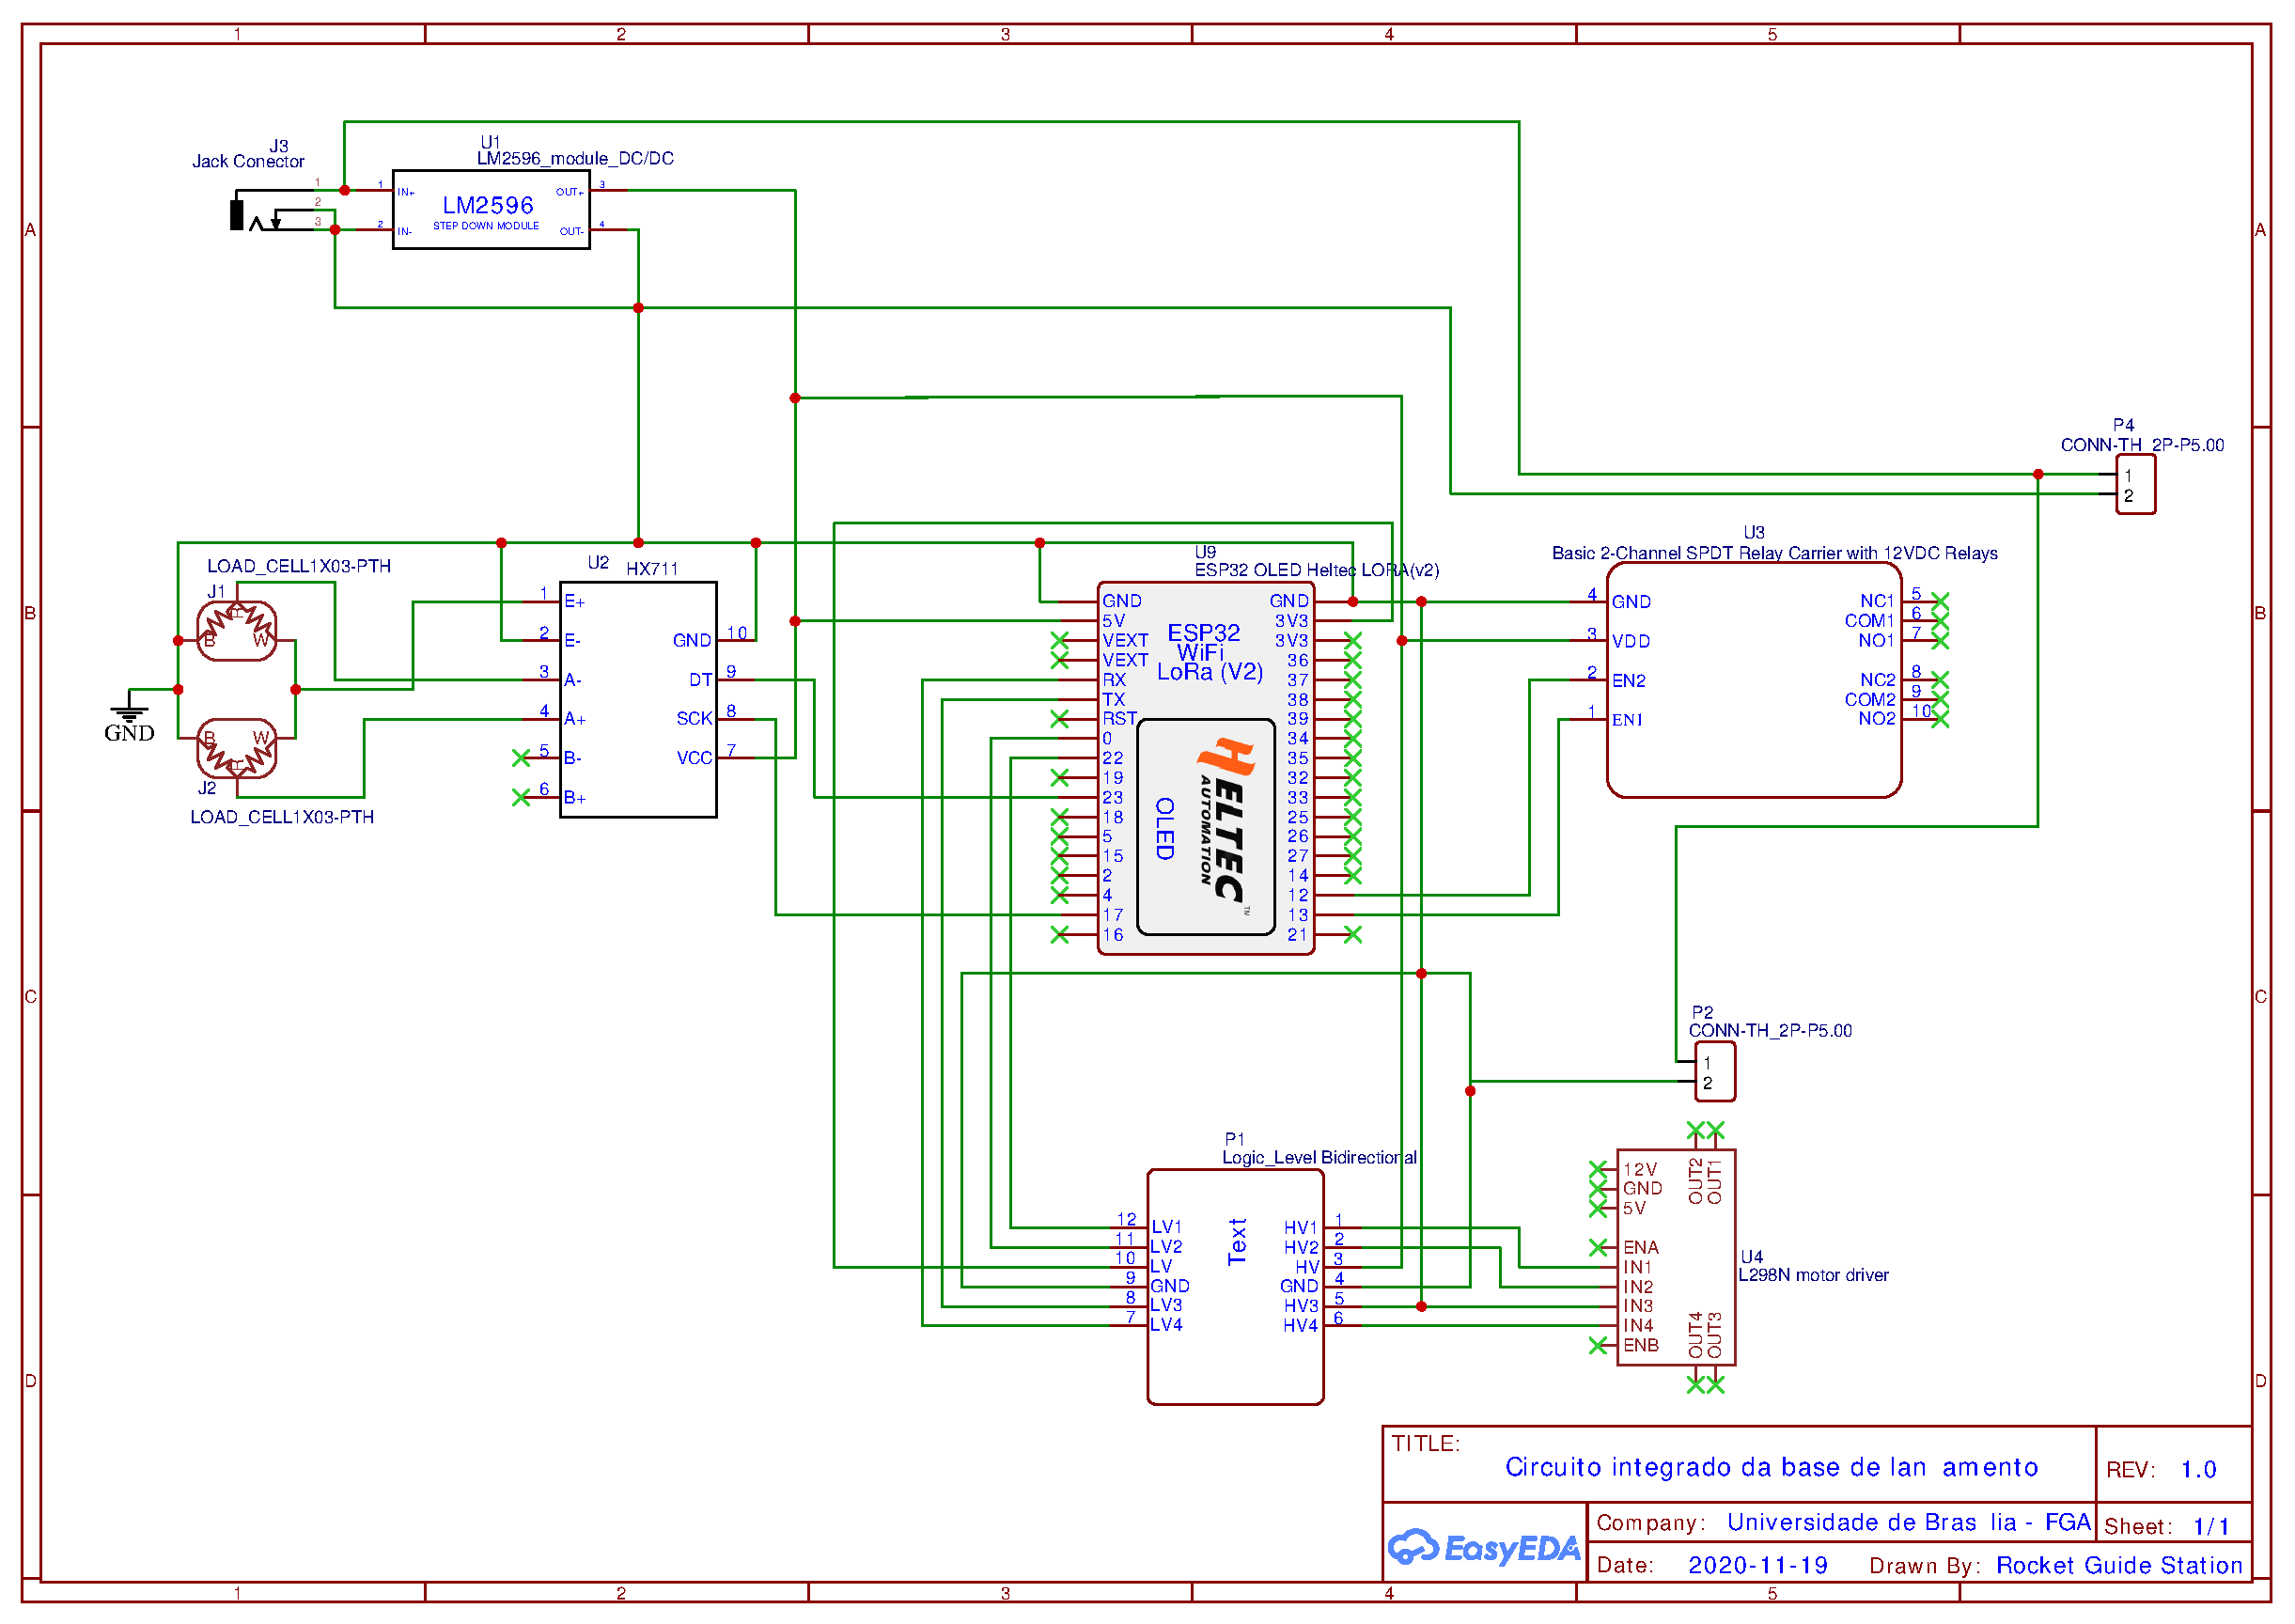
\includegraphics[scale=0.35]{figuras/PDFs/final eletronica/Schematic_base de lançamento.pdf}
  \caption{Diagrama esquemático do circuito interno da base de lançamento.} 
  {\footnotesize Fonte:Autor} 
  \label{fig:Diagrama esquematico do circuito interno da base de lancamento}
\end{figure}

\begin{figure}[H]
  \centering
  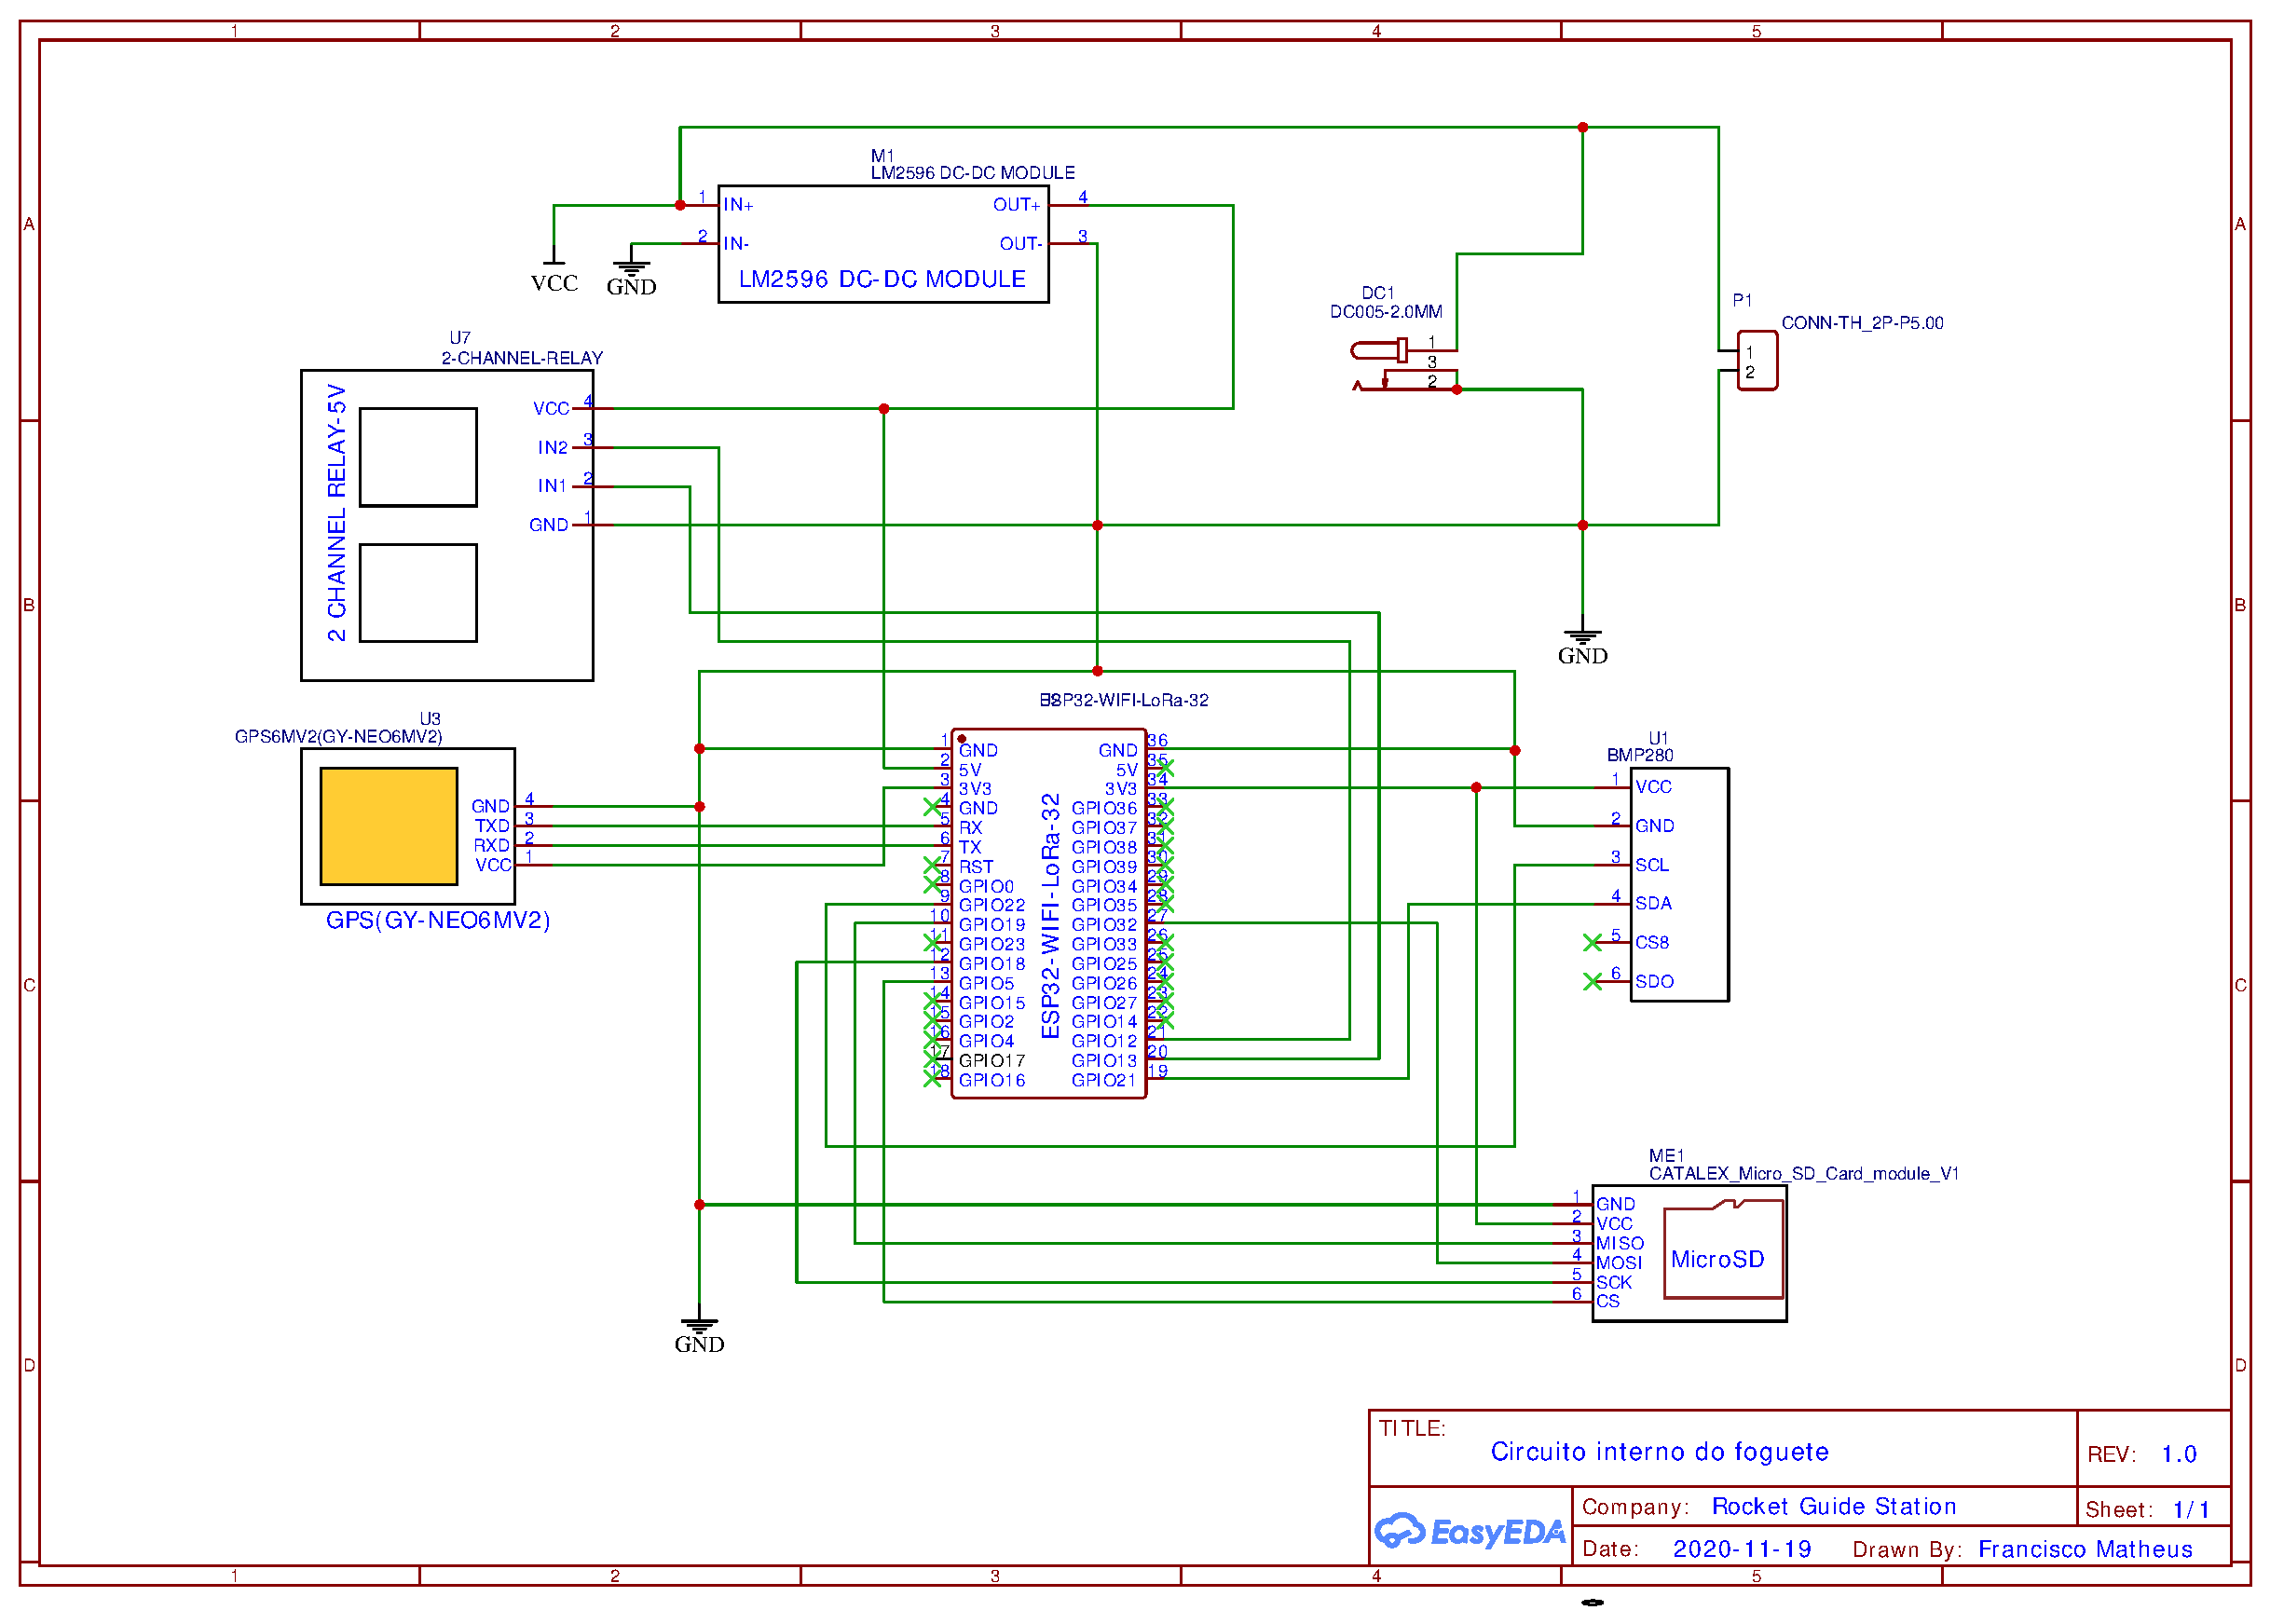
\includegraphics[scale=0.35]{figuras/PDFs/final eletronica/Schematic_Esquemático foguete.pdf}
  \caption{Diagrama esquemático do circuito interno do foguete. } 
  {\footnotesize Fonte:Autor} 
  \label{fig:Diagrama esquematico do circuito interno do foguete}
\end{figure}

\begin{figure}[H]
  \centering
  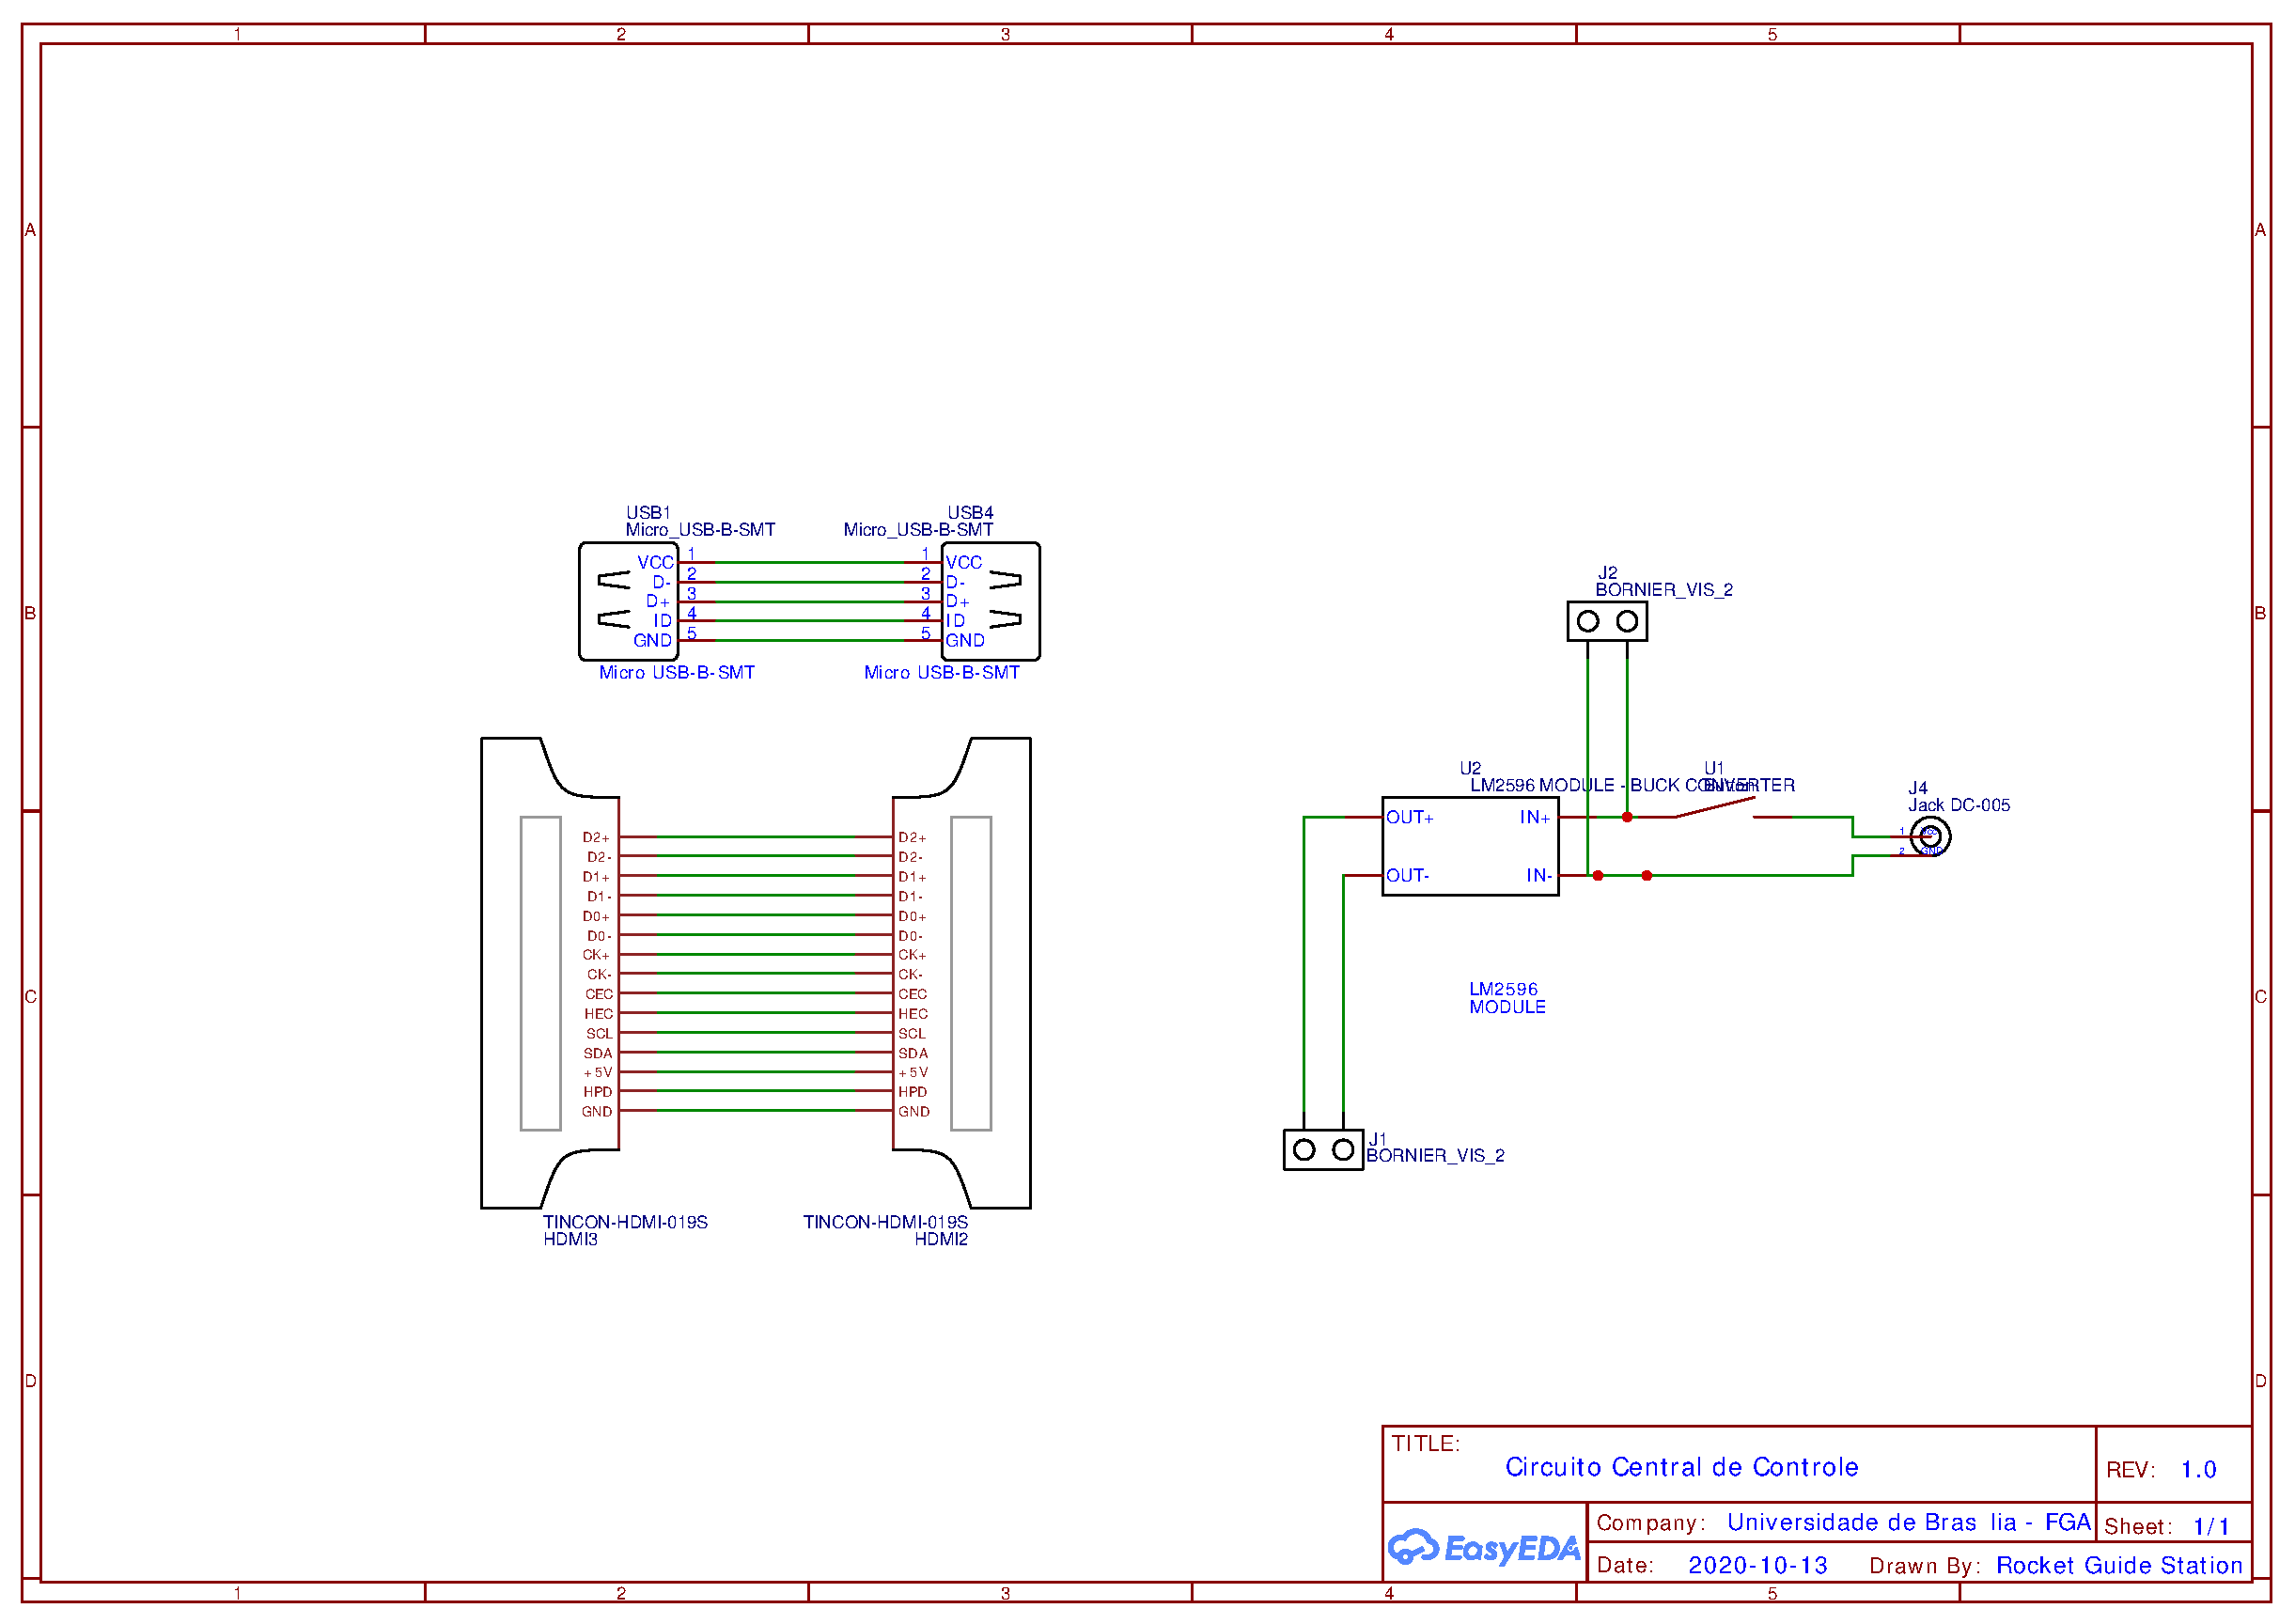
\includegraphics[scale=0.35]{figuras/PDFs/final eletronica/Schematic_maleta final.pdf}
  \caption{Diagrama esquemático do circuito da central de controle do usuário.} 
  {\footnotesize Fonte:Autor} 
  \label{fig:Diagrama esquemático do circuito da central de controle do usuário}
\end{figure}

\section{Placa de circuito impresso}

\par Para melhor funcionamento  e durabilidade do circuito, é necessária a criação do desenho de placa de circuito impresso, conhecido como PCI, que é gerido por regras que visam garantir a qualidade do funcionamento do circuito IPC-2221B \cite{IPC-2221}, visando a disposição dos componentes para melhor acomodação mecânica e eletromagnética, a fim de evitar interferências no circuito.
\par Basicamente, é constituída por uma base de um material isolante, geralmente fenolite ou fibra de vidro, revestida por uma fina camada de cobre na sua superfície, onde ocorre as ligações entres os componente eletrônicos que podem ser do tipo PTH ou SMD\cite{pci}. 

\par As placas utilizadas nesse projeto serão feitas de modo a acomodar componentes do tipo PTH, ou seja, componentes que serão inseridos na placa através de um furo denominado de pads, sendo necessário uma acurácia para não errar no distanciamento dos furos, evitando assim mal posicionamento dos componentes eletrônicos.
\par Outro levantamento importante que é necessário fazer no projeto de uma PCI é a largura das trilha, que são responsáveis pelas conexões elétricas entre os componentes, a qual é determinada pela corrente que irá passar pela trilha e pela espessura da trilha de cobre  e a temperatura \cite{ TecnicasdeProjetosPCI}. Os cálculos das trilhas foram feitos no site \href{https://pcbbrasil.com.br/calculo-trilha-pcb.php}{PCBBRASIL} que segue os critérios da norma IPC-2221B para confecção de placas de circuito impresso.
\par Para a confecção da placa de circuito impresso foi gerado o arquivo Gerber de cada placa de circuito impresso, sendo gerado um arquivo em formato ZIP disponível em \href{https://drive.google.com/drive/folders/1P1pQGE_zuSLOB5qd8zfESWqLDwtyoRKd?usp=sharing}{ Arquivos Gerber}. Para a visualização dos arquivos Gerber é necessário a utilização de um programa de prototipagem de placas de circuito impresso ou um visualizador desse tipo de arquivo disponível para \href{https://sourceforge.net/projects/gerbv/files/}{ \textbf{download}} no site do programa utilizado para o projeto EasyEda.

\subsection{Circuito interno do foguete}
\par Na figura \ref{fig:Diagrama esquematico do circuito interno do foguete}, está representado o circuito interno do foguete. Assim, na figura \ref{fig:PCIFOGUETE}, encontra-se o  projeto mecânico da placa de circuito impresso com as dimensões para sua fabricação. Foram adicionados cinco buracos na PCI no intuito de facilitar sua fixação dentro do foguete com parafusos de diâmetro de 5mm. Na figura \ref{fig:PCB_FOGUETE}, por sua vez, é apresentado o modelo 3D da PCI com com o sistema de alimentação à esquerda da placa, separado dos outros componentes a fim de evitar interferência eletromagnética no restante da placa. Foi adicionado a essa placa esse sistema para garantir a tensão adequada para os componentes. 
\par A placa a ser produzida possui espessura padrão de 1,6mm, com tolerância nominal de $\frac{+}{-}$ 0,13mm. Nessa PCB específica, são utilizadas duas camadas de cobre para as trilhas; portanto, serão feitas trilhas tanto na \textit{Top Layer} quanto na \textit{Bottom Layer}, ou seja, \textit{multilayer}, garantindo uma melhor distribuição das trilhas. Por ser um módulo que vai dentro do foguete, inicialmente foi pensado em usar componentes do tipo PTH e a plaquinha de desenvolvimento da ESP32Lora, da Heltec, pois não são feitos muitos lançamentos. A ideia é utilizar primeiramente uma PCB nesse formato para testes e melhorias no projeto, antes de confeccionar uma placa mais enxuta com componentes SMD. 
\par Para essa versão inicial das placas de circuito impresso, seriam feitas de fenolite (FR2), que é um material mais barato para a confecção e quando tiver os componentes testados será feito em material de vibra de vidro(FR4)\cite{CONCEITOpci}.

\begin{figure}[H]
  \centering
  \includegraphics[width=\textwidth]{figuras/PDFs/final eletronica/PCB_PCB_interna do foguete.png}
  \caption{Dimensões da PCI do circuito interno do foguete.} 
  {\footnotesize Fonte : Autor } 
  \label{fig:PCIFOGUETE}
\end{figure}

\begin{figure}[H]
  \centering
  \includegraphics[scale=0.4]{figuras/PDFs/final eletronica/foguete_top.png}.
    \includegraphics[scale=0.4]{figuras/PDFs/final eletronica/foguete_bottom.png}
  \caption{PCI do circuito interno do foguete.} 
  {\footnotesize Fonte : Autor } 
  \label{fig:PCB_FOGUETE}
\end{figure}


\subsection{Circuito na base de lançamento}
\label{sec:base_de_lancamento}

Objetivando reduzir o número de fios e cabos utilizados no circuito da base de lançamento, assim como obter a menor ocupação de volume de circuitaria e componentes, foi criado o modelo de PCI com base no circuito integrado citado na figura \ref{fig:Diagrama esquematico do circuito interno da base de lancamento}. Foi optado o modelo \textit{Bottom Layer} para as trilhas da PCI, ou seja, contém apenas uma camada de cobre.

A figura \ref{fig:PCB_BASE_LANCAMENTO_DES} mostra o desenho da PCI, junto com suas cotas de dimensões definidas, que foram de 88mm x 109mm. Os buracos nos cantos da PCB, com diâmetro de 4mm e distâncias das bordas de 3mm, servem pra fixação da placa na estrutura da base.

\begin{figure}[H]
  \centering
  \includegraphics[width=\textwidth]{figuras/PDFs/final eletronica/PCB_BASE_FINAL.png}
  \caption{ Dimensões da PCI do circuito interno da base de lançamento. } 
  {\footnotesize Fonte : Autor } 
  \label{fig:PCB_BASE_LANCAMENTO_DES}
\end{figure}

A figura \ref{fig:PCB_BASE_LANCAMENTO} apresenta a visão frontal da PCI, onde é possível visualizar a posição dos componentes, tais como encaixes dos pinos e os bornes dispostos nas extremidades, e a visão traseira da PCI, onde se encontra a camada de fundo (\textit{Bottom Layer}), com as trilhas do circuito.

\begin{figure}[H]
  \centering
  \includegraphics[scale=0.4]{figuras/PDFs/final eletronica/BASE_TOP.png}
    \includegraphics[scale=0.4]{figuras/PDFs/final eletronica/BASE_BOTTOM.png}
  \caption{PCI do circuito interno da base de lançamento } 
  {\footnotesize Fonte : Autor } 
  \label{fig:PCB_BASE_LANCAMENTO}
\end{figure}

\subsection{Circuito na base de controle central}

A ideia dessa PCI é reduzir o número de cabos utilizados dentro da maleta do usuário.
De acordo com o espaço e a disposição dos componentes mostrado na figura  \ref{fig:Disposicao dos Componentes} e na figura \ref{fig:PCB_controle} pensou-se em fazer uma placa de modo que os módulos sejam encaixados nas laterais da PCI. Para isso foi verificado todos desenhos técnicos dos componentes, mapeando então os conectores  por meio dessas medidas fornecidas pelo fabricante. Os conectores precisarão ser do tipo macho para que o encaixe seja realizado. Isso traz vantagens: caso algum módulo sofra dano, bastará  desconectá-lo e realizar a troca.

\begin{figure}[H]
  \centering
  \includegraphics[scale=0.5]{figuras/PCB_Maleta.png}
  \caption{ Dimensões da PCI do circuito da central de controle.} 
  {\footnotesize Fonte : Autor } 
  \label{fig:PCIMaleta}
\end{figure}

\begin{figure}[H]
  \centering
  \includegraphics[scale=0.4]{figuras/PDFs/final eletronica/maleta_top.png}
    \includegraphics[scale=0.4]{figuras/PDFs/final eletronica/maleta_bottom.png}
  \caption{PCI do circuito interno do foguete. } 
  {\footnotesize Fonte : Autor } 
  \label{fig:PCB_controle}
\end{figure}

\section{Energia}

A solução de energia do projeto consiste no dimensionamento de baterias que atendam às especificações e requisitos do sistema, tanto dos dispositivos eletrônicos quanto do sistema de ignição e lançamento. Além disso, será projetado um carregador de bateria para tornar contínuo o uso do equipamento.

Para dimensionar o consumo do sistema, foi observado o gasto energético dos componentes eletrônicos, levando em conta que o projeto precisa de uma autonomia de, no mínimo, duas horas de uso sem a possibilidade de ter como fonte de energia a rede elétrica.

Anteriormente, ao dimensionar o sistema de alimentação do projeto, foi definido que seria utilizada apenas uma bateria que alimentasse todos os componentes. Porém, ao avaliar melhor as necessidades do projeto, em especial a distância de segurança (500m) entre o usuário e a base de lançamento do foguete, optou-se por dimensionar dois sistemas, de forma a eliminar a utilização de cabos para alimentar os componentes que precisariam estar na base.

A utilização de cabos entre a base e o sistema de controle, além de não ser viável do ponto de vista do usuário, também provocaria impactos a serem considerados no projeto, como a queda de tensão atrelada a um cabo de grande extensão como o que seria necessário.

Sendo assim, para aumentar a qualidade e melhorar a usabilidade do produto, foi definido que o projeto será composto por dois sistemas: o sistema de controle e o sistema da base. Cada sistema será alimentado eletricamente de forma individual. Os dois sistemas estarão interligados por telemetria, conforme descrito na solução de eletrônica, e serão controlados pelo usuário, que utilizará o sistema de controle (maleta) a uma distância segura da base de lançamento.

\subsection{Ignição}
\label{sec:ignição}

Para dimensionar o sistema de alimentação elétrica do projeto, é necessário realizar o dimensionamento do consumo de potência do ignitor, que faz parte do sistema da base de lançamento. O tipo de ignitor utilizado pela \textit{{Equipe Capital Rocket Team}} é o fio de Níquel Cromo (Ni-Cr), os cálculos foram realizados com base nesse tipo de ignitor.

Para o ignitor de Níquel Cromo foi considerado o diâmetro de $0,8 mm^2$ e temperatura de ignição de 300ºC, a \textit{Capital Rocket Team} não dispunha dessas informações, mas esses foram os parâmetros mais comuns encontrados para esse tipo de sistema \cite{edufer2020}.  

No site do fabricante \cite{ignitor}, há uma tabela que permite, com a entrada desses dados, obter a resistência (em Ohm/m). A partir desse dado, utilizando a primeira Lei de Ohm, com o valor de tensão fornecido pela bateria (12V) será calculada a corrente consumida pelo ignitor.

A resistência obtida por meio da tabela do fabricante é de 2,23 Ohms/m, considerando um enrolamento de 1m, a resistência do ignitor é 2,23 Ohms. A corrente pode ser descrita de acordo com a primeira Lei de Ohm:

\begin{center}
\begin{equation}
 I = \frac{V} {R} 
 \end{equation}
 
 \begin{equation}
 I = \frac{12} {0,23}
 \end{equation}
 
 \begin{equation}
 I = 5,38 A
\end{equation}
\end{center}

Com o valor da corrente obtido e com base na relação entre corrente, tensão e potência, pode ser calculada a potência consumida.

\begin{center}
\begin{equation}\label{m}
	P = I \times V 
    \end{equation}
    
 \begin{equation}
  P =  5,38 \times 12 
  \end{equation}
  
  \begin{equation}
  P = 64,56 W 
\end{equation}
\end{center}

O ignitor será utilizado somente uma vez a cada lançamento, e apenas para o momento de ignição do foguete. Para fins de segurança, de forma a garantir a autonomia do sistema, será adotado o tempo de utilização de 15 minutos.

\subsection{Consumo dos sistemas}

Como dito anteriormente o projeto é separado por dois sistemas a maleta e a base de lançamento. Nas tabelas \ref{tab:consumo1} e \ref{tab:consumo2} é apresentado o consumo dos principais componentes elétricos e eletrônicos de cada um dos dois sistemas e uma estimativa do período que cada componente será utilizado durante um lançamento. 

\begin{center}
\begin{table}[H]
\centering
\begin{tabular}{ |m{4cm}|m{2cm}|m{2cm}|m{2cm}|m{3cm}|} 
\hline
\textbf{Componentes}&\textbf{Tensão} & \textbf{Corrente}& \textbf{Potência} & \textbf{Tempo de Utilização}\\ 
 \hline
 Tela & 12V & 1A & 12W & 2h30m\\
  \hline
Jetson Nano Developer Kit & 5V & 2A & 10W & 2h30m\\
  \hline
 Teclado e botões & 5V & 250 mA & 1,25W & 2h30m\\ 
  \hline
 Módulo LORA - maleta & 5V & 500mA & 2,5W &2h30m\\ 
 \hline
 
 \hline
\end{tabular}
\caption{Consumo elétrico dos componentes da maleta.}
\label{tab:consumo1}
\end{table}
\end{center}

Com base na tabela \ref{tab:consumo1}, o somatório de potências do sistema é de 25,75W. Será utilizado o valor de 30 W por segurança. O lançamento de um foguete tem duração média de 2 horas, o valor utilizado será de 2 horas e 30 minutos, por segurança.

Sendo assim, o somatório da potência é multiplicado pelo tempo em horas.

\begin{equation}
    30W \times 2,5h = 75 Wh
\end{equation}

\begin{center}
\begin{table}[H]
\centering
\begin{tabular}{ |m{4cm}|m{2cm}|m{2cm}|m{2cm}|m{3cm}|} 
\hline
\textbf{ Componentes }&\textbf{ Tensão} & \textbf{Corrente }& \textbf{Potência} & \textbf{Tempo de Utilização}\\ 
 \hline
 Módulo LORA - base & 5V & 500mA & 2,5W & 2h5m\\ 
 \hline
 Ignitor (Ni-Cr) & 12V & 5,38A & 64,56W & 15m \\
 \hline
 Atuadores (3x) & 12V & 3.9A & 46,8W & 15m \\ 
 \hline
\end{tabular}
\caption{Consumo elétrico dos componentes da base de lançamento.}
\label{tab:consumo2}
\end{table}
\end{center}

Para a alimentação dos componentes, vão ser utilizadas tensões contínuas de 5 V e 12 V. A bateria a ser utilizada será de 12V, já que a maior tensão dentre os equipamentos.

Com base na tabela \ref{tab:consumo2}, o somatório de potências do sistema é de 113,86W; porém, o valor utilizado de 2 horas e 30 minutos será usado apenas para o módulo, o ignitor e os três atuadores funcionam apenas nos primeiros minutos do lançamento. Por isso para calcular a potência destes será usado o tempo de 15 minutos.

Para o módulo:
\begin{equation}
    2,5W \times 2,5h = 6,25 Wh
\end{equation}

Para ignitor e atuadores:

\begin{equation}
    111,36W \times 0,25h = 27,84 Wh
\end{equation}

A potência total consumida pela base é :

\begin{equation}
    6,25Wh + 27,84Wh = 34,09 Wh
\end{equation}

Essa será a energia necessária consumida para a autonomia especificada. Por segurança será considerado o valor de 40 Wh.
Pela Lei de Ohm temos:

\begin{equation}
   I =  \frac{P}{V}
   \end{equation}
   
   \begin{equation}
      I =  \frac{34,09}{12}
   \end{equation}
   
  \begin{equation}   
   I = 3,33 Ah
 \end{equation}

\subsection{Baterias}

As duas baterias serão de 12V, já que esta é a maior tensão dentre todos os equipamentos nos dois sistemas.

Dentre os tipos mais comuns de baterias no mercado, estão as de chumbo-ácido e de íons de lítio. 

A bateria de chumbo-ácido é a mais comum, é comercializada há mais tempo e requer pouca manutenção. Esse modelo não possui efeito memória, que diminui a capacidade de carga. Porém, o chumbo, além de ser tóxico, possui baixa densidade de energia,  o que limita sua aplicação a sistemas portáteis leves \cite{baterias}.

As baterias de íons de lítio tem como componente principal o lítio, que é um metal leve e com grande potencial eletroquímico, o que proporciona uma grande densidade de energia. Esse tipo de bateria também não possui efeito memória, importante em sistemas que sofrerão cargas e descargas frequentemente. Porém, essa tecnologia é mais recente, e o custo das baterias de íons de lítio é mais elevado \cite{baterias}. 

\subsubsection{Sistema de controle - maleta} 

Para a bateria do sistema de controle, em formato de maleta, buscou-se no mercado o tipo de bateria mais compacto possível de forma a atender a carga dimensionada, o modelo mais adequado encontrado foi o modelo de baterias de notebook, que é de íons de lítio. 

De acordo com o dimensionamento, a potência consumida é de 75Wh. Por questões de segurança será considerada uma descarga máxima de 80\%, sendo assim a capacidade da bateria será:

Capacidade em Wh
\begin{equation}
    75/0,8 = 93,75 Wh
\end{equation}

A capacidade necessária para esse sistema é de 93,75 Wh. Foi selecionada uma bateria da fabricante Dell, de 9 células e capacidade de 97 Wh, com as características a seguir:

Peso: 508,02 g

Dimensões

- Profundidade: 71,79 mm 

- Altura: 20,00 mm 

- Largura: 214,00 mm  


Na Figura \ref{fig:bateriamaleta} é apresentada a bateria selecionada para a maleta.

\begin{figure}[!h]
	\centering
		\includegraphics[keepaspectratio=true,scale=1]{figuras/bateria_maleta.jpg}
	\caption{Bateria selecionada para o sistema de controle. Fonte: \cite{figura_bateria_maleta}} 
	\label{fig:bateriamaleta}
	\end{figure}

\subsubsection{Sistema da base de lançamento} 

A capacidade calculada para o sistema da base de lançamento foi de 3,33 Ah. De acordo com o fabricante a capacidade da bateria deve ser mantida entre 50\% - 60\%, por segurança e de forma a prolongar a vida útil do equipamento. Considerando então uma descarga máxima de 40\% a capacidade da bateria será:

Capacidade em Ah
\begin{equation}
     3,33/0,4 = 8,33 Ah
\end{equation}

A capacidade necessária para esse sistema é de 8,33 Ah, a bateria selecionada deve ter capacidade de 9 a 10 Ah. Como mencionado anteriormente, as baterias mais comuns no mercado são de chumbo-ácido e de lítio. Dessa forma, buscou-se fabricantes que possuíssem os dois tipos de bateria, com a capacidade necessária para o sistema, para realizar uma comparação e selecionar a mais adequada.

Durante as pesquisas encontrou-se informações mais completas do fabricante \textit{Unipower}, esse fabricante possui um modelo de bateria de chumbo-ácido de 12V e 9Ah e um modelo de lítio, de 12V e 10Ah. Ambas as baterias possuem as mesmas dimensões $(100mm \times 151mm \times 65mm)$, porém, a bateria de chumbo-ácido pesa 2,5 kg enquanto a bateria de lítio pesa 1,5 kg. Como o sistema deve ser portátil é importante que ele seja o mais leve e compacto possível, dessa forma foi escolhido o modelo de lítio, que é mais leve e tem maior capacidade. O fabricante \textit{Unipower} trabalha com um tipo específico de baterias de íons de lítio, as baterias de lítio ferro fosfato.

A bateria selecionada é a Bateria Lítio Ferro Fosfato - LiFePO4, modelo UPLFP12-10.  Na Figura \ref{fig:bateriabase} é apresentada a bateria selecionada para a base de lançamento. 

\begin{figure}[!h]
	\centering
	\label{bateria_base}
		\includegraphics[keepaspectratio=true,scale=0.6]{figuras/bateria_base.jpg}
	\caption{Bateria selecionada para a base de lançamento. }
	{\footnotesize Fonte: \cite{datasheet_bateria}}
	\label{fig:bateriabase}
\end{figure}

\subsection{Regulador de tensão}

Como as fonte de tensão são de 12V, serão utilizados módulos “\textit{step down}” para regular as tensões direcionadas para alguns componentes do sistema. No projeto, será utilizado o módulo regulador de tensão modelo LM2596 apresentado na figura \ref{fig:regulador tensao}, pois este possui uma ampla faixa de tensões de entrada e pode ser regulado para uma tensão específica de saída com uma boa eficiência \cite{datasheet_regulador}.

A faixa de tensão utilizada será de 5V, de acordo com a necessidade de cada dispositivo eletrônico no sistema.

\begin{figure}[!h]
	\centering
	\label{regulador_tensão}
		\includegraphics[keepaspectratio=true,scale=1]{figuras/regulador_de_tensão.jpg}
	\caption{Regulador de tensão modelo LM2596.}
	\label{fig:regulador tensao}
\end{figure}

\subsection{Funcionamento do sistema de alimentação}

A partir da definição de todos os equipamentos é possível visualizar o funcionamento de cada sistema de alimentação.  

O diagrama em blocos do sistema de controle pode ser observado na Figura \ref{fig:blocosmaleta}.

\begin{figure}[!h]
	\centering
		\includegraphics[keepaspectratio=true,scale=0.6]{figuras/blocos_maleta.jpeg}
	\caption{Diagrama em blocos do sistema de controle - maleta.}
	\label{fig:blocosmaleta}
\end{figure}

Nesse sistema a bateria alimenta diretamente a placa de controle da tela e o módulo regulador de tensão. Nesse ponto de alimentação está inserido um botão interruptor, de forma a ligar ou desligar o sistema como um todo.

O regulador de tensão, por sua vez, alimenta o \textit{Single Board Computer} que se conecta ao teclado e ao módulo LORA via cabo USB, além disso, o \textit{Single Board Computer} se conecta a placa de controle da tela via cabo HDMI. 

O diagrama em blocos do sistema da base de lançamento pode ser observado na Figura \ref{fig:blocos_base}.

\begin{figure}[!h]
	\centering
		\includegraphics[keepaspectratio=true,scale=0.6]{figuras/blocos_base.jpeg}
	\caption{Diagrama em blocos da base de lançamento.}
	\label{fig:blocos_base}
\end{figure}

No sistema da base de lançamento a bateria alimenta diretamente o ignitor, o circuito ponte H, o módulo relé 2 canais e o módulo regulador de tensão. Nesse sistema, não foi inserido o botão liga/desliga, pois os componentes serão ativados por meio do sistema de controle.

Os atuadores das válvulas são alimentados por meio do circuito ponte H, o atuador do engate é alimentado por meio do relé 2 canais, o relé e o circuito ponte H estão conectados com o módulo LORA, que é alimentado por meio do módulo regulador de tensão.

É possível observar ainda, em ambos os sistemas, o esquema de carregamento da bateria, a conexão entre o carregador e a bateria está representada por um interruptor, pois essa conexão não é fixa, e será realizada apenas nos momentos de carregamento de cada bateria. A conexão será feita por meio de um conector \textit{Jack}, presente em cada uma das estruturas.

\subsection{Carregador de bateria}

A solução inicial para o sistema consistia em realizar o carregamento da bateria \textit{off grid}, ou seja, sem conexão com a rede elétrica, a partir do uso de placas fotovoltaicas. Porém, ao analisar as condições de operação do sistema, em especial o tempo de operação, que é previsto para no máximo 2 horas, concluiu-se que a solução mais adequada seria realizar o carregamento \textit{on grid}, conectado à rede elétrica, a partir de um carregador de bateria, a ser projetado.

Dessa forma, as baterias, tanto da maleta quanto da base, serão levada com carga completa até o local de lançamento, todo o sistema poderá ser alimentado a partir delas, e, ao retornar para um local com conexão à rede elétrica, as baterias poderão ser recarregadas, e o sistema estará pronto para o próximo uso.

Como as duas baterias são de Íon-Lítio, será projetado um único carregador que seja compatível com as especificações técnicas das duas baterias usadas no projeto, a tensão de saída deve ser no máximo de 14,6V e a corrente máxima de saída 10A.

\subsubsection{Fonte de Alimentação}

A fonte de alimentação será a  responsável por entregar a tensão e a corrente necessária para carregar as duas baterias do sistema, como o carregador será ligado à rede elétrica, foi projetado um circuito capaz de converter corrente alternada (rede elétrica) para corrente contínua (usada no projeto) e fazer a redução de tensão (no caso, de 220V para 30V). Para isso, foi inserido um transformador e um retificador de onda completa.

\textbf{Transformador}
    
Um transformador é constituído basicamente de dois enrolamentos onde o fluxo magnético, variável, produzido em um age sobre o outro. O enrolamento no qual a fonte é aplicada é o primário do transformador e o enrolamento onde a carga é conectada é o secundário \cite{transformadores}.

Para o projeto, deseja-se a utilização de um transformador de tensão (com \textit{center-tapped}), que será responsável por abaixar a tensão. Em nosso caso, a tensão de entrada será a tensão fornecida pela rede, que é de 220V alternada, e a tensão de saída será a tensão desejada para o funcionamento do projeto, que será de 30V, ainda alternada na saída do transformador.

\textbf{Retificador de onda completa}

Como a tensão na saída do transformador é alternada é necessário um retificador para torná-la contínua, o Retificador de onda completa consiste no uso de 2 diodos acoplados ao transformador que contenha \textit{center-tapped}, para garantir a retificação de onda completa. 

Os diodos são dispositivos eletrônicos que permitem a passagem de corrente elétrica em apenas um sentido. Eles só permitem a passagem de corrente elétrica quando esta é polarizada diretamente, ou seja, quando o polo positivo da fonte entra em contato com o polo positivo do diodo \cite{retificador}. No circuito, o diodo funciona de acordo com a figura \ref{fig:retificador}

\begin{figure}[!h]
	\centering
		\includegraphics[keepaspectratio=true,scale=0.5]{figuras/retificador_completo.JPG}
	\caption{Esquemático de um retificador de onda completa. Fonte: \cite{retificador}}
	\label{fig:retificador}
\end{figure}

\subsubsection{Circuito de carregamento}

O carregador de baterias de lítio íon é um dispositivo limitador de tensão similar ao carregador de baterias de chumbo-ácido. A diferença está em uma maior tensão por célula, uma tolerância de tensão menor e a ausência de carga de flutuação ou pulsante quando a carga completa é alcançada \cite{bateria_litio}.

O tempo de carga de todas as baterias de Lítio-Íon, quando carregadas a uma corrente inicial de 1 C, é de aproximadamente 3 horas. A bateria permanece fria durante a carga. A carga completa é alcançada depois que a tensão alcança o limiar de tensão superior e a corrente ter caído e se igualado a 3\% da corrente de carga nominal. Na figura \ref{fig:curvacarga}, é mostrada a curva de carga de uma bateria de Lítio íon.

\begin{figure}[!h]
	\centering
		\includegraphics[keepaspectratio=true,scale=0.5]{figuras/Curva_carga.JPG}
	\caption{Curva de carga da bateria de Lítio íon. Fonte: \cite{bateria_litio}}
	\label{fig:curvacarga}
\end{figure}

Baterias de lítio íon são projetadas para operar seguramente dentro da sua tensão normal de operação, mas tornam-se cada vez mais instáveis se carregadas em voltagens maiores. Por esse motivo, é importante que haja circuitos internos de controle de tensão que interrompem a bateria em subtensão ou sobre tensão \cite{bateria_litio}.

Foi criado, usando o software Proteus, o circuito de carregamento das baterias (já inserida a fonte de alimentação). O apêndice \ref{diag_eletrico} contém o desenho do circuito criado. Nas figuras \ref{fig:bateriatensao} e \ref{fig:bateriacorrente} são apresentados os testes de simulação do circuito contendo as medições de tensão e corrente.

\begin{figure}[!h]
	\centering
		\includegraphics[keepaspectratio=true,scale=0.5]{figuras/Medição - Tensão.PNG}
	\caption{Medição de tensão no circuito carregador. Fonte: \cite{retificador}}
	\label{fig:bateriatensao}
\end{figure}

\begin{figure}[!h]
	\centering
		\includegraphics[keepaspectratio=true,scale=0.5]{figuras/Medição - Corrente.PNG}
	\caption{Medição de corrente no circuito carregador.}
	\label{fig:bateriacorrente}
\end{figure}

Observando as medições, é possível comprovar que, ao final do circuito, a bateria recebe uma tensão de 13.6V e uma corrente de 1A, capaz então de recarregá-la até 12V. O circuito de carregamento faz o controle da tensão para manter a carga, caso, depois de cheia, se a bateria perder a carga, o carregador reativa-se até ficar novamente com a carga completa. Desse modo, a bateria pode estar ligada de forma permanente ao carregador, mantendo a carga completa sem nenhum dano a bateria ou ao circuito.

\subsection{Dimensionamento dos condutores}

Para questões de dimensionamento dos condutores, o projeto será separado em três partes: carregador, maleta e base. Para determinar o diâmetro da seção transversal dos condutores utilizados no projeto, foi usada a norma NBR 5410/2004 \cite{NBR5410}. Segundo a norma, é preciso levar em conta dois parâmetros para decidir o diâmetro dos condutores: seção mínima de acordo com o método de instalação e capacidade de condução de corrente. A seção final dos condutores é dada pela maior seção entre os dois parâmetros encontrados.

O primeiro parâmetro é obtido por meio de uma análise das condições apresentadas pela norma, de acordo com o tipo de linha e utilização do circuito. No nosso caso, serão utilizados fios de cobre. Na tabela 47 da norma, são mostrados valores mínimos para a seção, a depender da utilização do circuito. De lá, foram tirados os seguintes dados:

\begin{itemize}
    \item Circuito carregador - Tipo: Circuitos de força - Seção mínima: $2,5mm^2$;
    \item Circuito maleta - Tipo: Linhas flexíveis para qualquer outra aplicação - Seção mínima: $0,75mm^2$
    \item Circuito base - Tipo: Linhas flexíveis para qualquer outra aplicação - Seção mínima: $0,75mm^2$
\end{itemize}

O segundo parâmetro leva em conta a corrente de projeto corrigida. Dessa forma, para cada parte do sistema geral, ter-se-á uma seção específica de condutor, uma vez que cada ramo apresenta uma potência diferente. A corrente de projeto corrigida é calculada segundo a equação abaixo:

\begin{equation}
    I_{c} = \frac{P}{V \times f_{p} \times FCA \times FCT}
\end{equation}

Onde:
\begin{itemize}
    \item [--] $I_{c}$ corrente de projeto corrigida;
    \item [--] $P$ potência requerida;
    \item [--] $V$ Tensão requerida;
    \item [--] $f_{p}$ fator de potência;
    \item [--] $FCA$ fator de correção de agrupamento;
    \item [--] $FCT$  fator de correção de temperatura.
\end{itemize}
Os fatores de correção a serem adotados para a determinação da corrente demandada em cada seção do circuito foram:

- Considerando que o lançamento acontece durante o dia em locais abertos, será considerada para a maleta e a base uma temperatura de 40ºC, um pouco mais alta que a ambiente, para segurança do projeto. De acordo com a tabela 40 da norma esta temperatura retorna um valor de FCT = 0.91 ;

- Será desconsiderado o agrupamento dos circuitos, levando o fator de correção por agrupamento a um valor unitário; 

- Será considerado um fator de potência unitário.


Para cada parte do projeto, a corrente corrigida será:

\begin{itemize}
    \item Circuito carregador
    Para o fluxo rede elétrica - fonte:
\begin{equation}
    I_{c} = \frac{1927,65W}{220V \times 1 \times 1 \times 1} = 8,762A
\end{equation}
Pela NBR 5410 tabela 37 a seção adequada é $0,5mm^2$

    Para o fluxo fonte - bateria:
\begin{equation}
    I_{c} = \frac{60W}{30V \times 1 \times 1 \times 1} = 2A
\end{equation}
Pela NBR 5410 tabela 37 a seção adequada é $0,5mm^2$  

    \item Circuito maleta
  \begin{equation}
    I_{c} = \frac{97W}{12V \times 1 \times 1 \times 0.91} = 8,88A
\end{equation}
Pela NBR 5410 tabela 37 a seção adequada é $0,5mm^2$  
        \item Circuito base
  \begin{equation}
    I_{c} = \frac{113,86W}{12V \times 1 \times 1 \times 0.91} = 10,42A
\end{equation}
Pela NBR 5410 tabela 37 a seção adequada é $0,75mm^2$ 
\end{itemize}

Após comparar os valores calculados com os do parâmetro de seção mínima baseados na norma, é mostrado na tabela \ref{tab:condutores} a seção final dos condutores em cada uma das partes.

\begin{center}
\begin{table}[H]
\centering
\begin{tabular}{ |m{5cm}|m{5cm}|} 
\hline
\textbf{ Circuito }&\textbf{ Seção dos condutores ($mm^2$)}\\ 
 \hline
 Carregador & 2,5 \\ 
 \hline
 Maleta & 0,75 \\
 \hline
Base & 0,75  \\ 
 \hline
\end{tabular}
\caption{Dimensionamento dos condutores do projeto.}
\label{tab:condutores}
\end{table}
\end{center}

\subsection{Plano de construção}

\subsubsection{Carregador}

Para construir o carregador de baterias, que poderá ser utilizado para recarregar as baterias dos dois sistemas projetados, deve ser seguido o projeto de circuito especificado no Apêndice \ref{diag_eletrico}. Os componentes estão descritos no projeto e na Tabela \ref{tab:custos} com os custos de cada um. 

A partir do desenho do circuito, o usuário deverá gerar uma placa de circuito impresso, onde os componentes devem ser inseridos e conectados utilizando o aparelho ferro de solda.

O fio de área de $2,5 mm^2$ deverá ser utilizado para realizar a conexão entre o \textit{plug} macho (tomada) e a entrada do transformador, e, entre a saída do circuito e o \textit{plug do conector DC Jack}.

\subsubsection{Sistema de controle e sistema da base de lançamento}

Com base nos diagramas em blocos na Figura \ref{fig:blocosmaleta} e Figura \ref{fig:blocos_base}, e do diagrama unifilar do sistema de controle e da base, Figura \ref{fig:diagrama_unifilar_01} e Figura \ref{fig:diagrama_unifilar_02} do Apêndice \ref{diag_eletrico}, é possível identificar as ligações entre os componentes de forma a construir o sistema de alimentação para ambas as estruturas.


O fio de área 0,75 mm² deverá ser utilizado para fazer as conexões elétricas entre os componentes.  A bateria deverá ser ligada ao \textit{conector DC Jack}, presente na estrutura, para que a conexão ao carregador possa ser realizada.

No sistema de controle, logo após a bateria, deve ser inserido o botão interruptor (chave gangorra). 




\section{Estrutura}

\par Baseado nos requisitos estruturais apresentados no PC01 e atualizados na tabela \ref{tab:Requisitos de Estrutura}, a solução de estrutura foi desenvolvida.

\begin{table}[H]
\centering
\begin{tabular}{ | m{2cm} | m{12cm}| } 
 \hline
 \textbf{Requisito} & \begin{center}\textbf{Descrição}
   
 \end{center} \\ 
 \hline
 RFEST01 & Ser de uso intuitivo para o usuário.\\
 & \\
\hline
 RFEST02 & Uma estrutura física compacta e portátil, que dê suporte aos componentes internos da estação. \\
 \hline
 RFEST03 & Material leve e resistente, capaz de proteger os componentes internos da estação de eventuais impactos e intempéries provenientes do ambiente e de seu deslocamento. \\
  \hline
RFEST04 & Uma segunda estrutura física compacta e portátil, voltada para o armazenamento do sistema de abastecimento. \\
\hline
RFEST05 & Ter um sistema de transmissão de torque do atuador para a válvula-esfera do sistema de abastecimento. \\
\hline
RFEST06 & Proteger o sistema eletrônico e não gerar interferência neste.  \\
\hline
RFEST07 & Estrutura interna acessível e de fácil manutenção. \\
\hline
RFEST08 & Sistema de abastecimento baseado nos componentes definidos pelo cliente. \\
\hline
\end{tabular}
\caption{Requisitos de Estrutura}
\label{tab:Requisitos de Estrutura}
\end{table}

\begin{figure}[!h]
	\centering
	\label{bateria_maleta}
		\includegraphics[width=0.7\textwidth]{figuras/estrutura.png}
	\caption{Solução estrutural}
	\label{soluçao_estrut}
	\end{figure}

\par O RGS necessita que todo o seu sistema seja portátil e suficiente para configurar e apoiar as missões de foguetes da CTR. Assim, durante sua concepção estrutural, o principal foco da equipe foi a mobilidade e a robustez para adequação às condições ambientais encontradas nos potenciais locais de lançamento e teste de foguetes. Por isso nossa solução estrutural deve ser equipada com todos os instrumentos necessários para o suporte eletrônico e de software responsáveis por rastrear e comandar o foguete durante o lançamento.

\par Dessa forma, nossa solução se divide em três frentes. A primeira é a maleta de usuário, onde ficarão os componentes eletrônicos e a interface de usuário de software (\ref{maleta_01}). Depois tem-se a maleta de suporte, responsável por abrigar os componentes para o abastecimento e a ignição do foguete à distância (\ref{maleta_02}). E, por fim, tem-se o sistema de abastecimento e ignição em si com seus componentes em uso integrados a outras partes do projeto (\ref{abastecimento}). Na figura \ref{soluçao_estrut} pode-se ver como o trabalho estrutural foi dividido.


\subsection{Maletas}

\par A solução estrutural inicial era de desenvolver apenas uma estrutura em formato de maleta, visando que ela fosse o bastante para o uso e carregamento de toda a solução. Porém, depois foi visto que a solução proposta demandaria do cliente o uso de um cabo de energia, muito superior aos comerciais, se tornando um empecilho para a usabilidade do produto. Além de que um cabo elétrico de grandes dimensões possui perda ao longo de sua transmissão, assim foi optado por desenvolver uma solução totalmente segura e sem fios para o conjunto de controle e de abastecimento. 

\par Fazendo-se então necessária a construção de uma segunda estrutura para comportar e transportar os elementos de abastecimento de modo que esse fique perto da base de lançamento, enquanto a outra estrutura fica em uma distância segura com o usuário.

\begin{figure}[!h]
	\centering
	\label{bateria_maleta}
		\includegraphics[width=1\textwidth]{figuras/antes_depois.png}
	\caption{Solução no PC1 e solução no PC2}
	\label{antes_depois}
	\end{figure}

\subsubsection{Especificações de materiais}
\label{sub:Especificações de materiais}

\par Durante a seleção de materiais, é necessária uma sistematização que permita analisar a vasta possibilidade de combinação de materiais que podem constituir determinado produto a fim de extrair um candidato vencedor, que cumpra com maior eficiência possível os requisitos da aplicação \cite{walterconteudo}.

\par Antes de apresentar a lista em si, é necessário evidenciar as características desejáveis para as estruturas que serão utilizadas na solução. Durante a etapa de escolha do material a ser utilizado, nem sempre é possível contemplar satisfatoriamente todos os aspectos necessários para aquela determinada finalidade. Por isso, tais aspectos são dispostos em ordem de relevância para o projeto, para que a escolha do material seja feita com embasamento teórico dentro da necessidade real do protótipo. 

\begin{enumerate}
    \item O fator mais relevante para a caixa da \textit{ground station} é o correto funcionamento no local de lançamento. A caixa deve estabelecer, por meio de ondas eletromagnéticas, comunicação mútua com o foguete e com o sistema de abastecimento de propelente durante todas as etapas de lançamento. Portanto, o material escolhido \textbf{não deve gerar interferência} nos sistemas de comunicação. 
    \item A usabilidade e a ergonomia vem a seguir, responsáveis por garantir que o usuário consiga ler, de forma clara e precisa, todos os parâmetros relevantes para a missão e que o auxiliará na tomada de decisão. Assim, \textbf{o material utilizado deve ser moldável} para que embarque os componentes necessários e os disponha de maneira adequada, respeitando as suas diferentes geometrias.
    \item O \textbf{custo} é o terceiro fator mais relevante, uma vez que a viabilidade de fabricação do protótipo está diretamente relacionada com seu valor final. Além do material ser acessível do ponto de vista financeiro, é desejável que ele permita agilidade em sua construção, dado que um material difícil de ser trabalhado pode gerar mais horas de trabalho, o que resulta no aumento do valor total da mão-de-obra e, por consequência, aumento do valor final do protótipo.
    \item Como quarta prioridade, a caixa deve ser resistente de maneira que eventuais quedas ou impactos com outros objetos não venha a interferir o seu correto funcionamento. Materiais com boa \textbf{resistência mecânica} podem contemplar tal característica.
    \item Por fim, a portabilidade se faz necessária devida à utilização da caixa ocorrer em lugares de acesso restrito. Logo, a caixa deve ser \textbf{leve e compacta} para facilitar o seu transporte.
\end{enumerate}

\par Visto os aspectos desejáveis, é apresentado a seguir o estudo de possíveis materiais a serem utilizados no protótipo, bem como a escolha final de uso.

\begin{itemize}
    \item \textbf{\textit{Medium Density Fiberboard} - MDF}
     \par O MDF é um material fabricado a partir da aglutinação de fibras de madeira com resina sintética – sendo as mais utilizadas à base de ureia formaldeído, tanino formaldeído e melamina ureia formaldeído –  posteriormente submetidas à prensagem em altas temperaturas  \cite{gomes}.  Sua composição permite que ondas eletromagnéticas possam fluir através dela.
     
    \par Sua superfície é plana e lisa, oferece alta usinabilidade para encaixar, entalhar, cortar, parafusar, perfurar e moldurar, além de reduzir o uso de tintas, vernizes e ótima aceitação de revestimentos \cite{CAMPOS}.
    
    \par O custo varia de acordo com a espessura da chapa. O valor do metro quadrado de uma chapa de 3 mm é R\$36,81. Já uma chapa de 6 mm custa R\$62,50 o metro quadrado.  Por possuir boa trabalhabilidade \cite{eleoterio2000propriedades}, o processo de construção pode apresentar satisfatória rapidez.  
    
    \par As características mecânicas específicas do material variam de acordo com o tipo de fibra e resina utilizadas. Em geral, são vantagens do MDF a alta relação entre resistência mecânica e massa específica, homogeneidade e ausência de defeitos como nós e desvios de grão \cite{eleoterio2000propriedades}. 
    
    \par De acordo com Silva e Gonçalves \cite{da2007avaliaccao}, os MDF são projetados para serem fabricados com densidades entre 0,5 e 0,8 $g/cm^3$. 
    
    \par Na tabela \ref{tab:mdf} é apresentado algumas das principais propriedades físicas e mecânicas de painéis MDF confeccionados com madeira de \textit{Eucalyptus grandis}.
    
\begin{table}[h]
\centering
\begin{tabular}{|l|l|}
\hline
Densidade              & 0,695 $g/cm^3$ \\ \hline
Módulo de elasticidade & 3776 $MPa$ \\ \hline
Módulo de ruptura      & 36,1 $MPa$ \\ \hline
Resistência a tração   & 1,01 $MPa$ \\ \hline
\end{tabular}
\caption{Propriedades do MDF}
\label{tab:mdf}
\end{table}

    \item \textbf{Polímero Reforçado com Fibra de Vidro - PRFV}
    
    \par É um material composto por uma matriz de resina sintética termofixa, como a Resina Epóxi, reforçada com estreitos filamentos flexíveis de vidro, cujo principal constituinte é a sílica \cite{pierin2005estudo}. O PRFV não gera interferência na comunicação com os sistemas. 
    
    \par Possui razoável manuseabilidade, pode ser cortado, perfurado e moldado, porém caso a caixa seja composta por várias peças o encaixe entre elas pode dificultar o processo de montagem.    
    
    \par O processo de fabricação é lento pois é necessária a fabricação do PRFV em si, ou seja, não é vendido o PRFV pronto para uso e sim os filamentos de vidro e a resina. Além disso, o PRFV deve ser confeccionado em um molde que deve ser previamente fabricado com o formato da peça final. O custo de material suficiente para produzir um metro quadrado de PRFV é de R\$52,90.  
    
    \par De acordo com Lin et al (1996), conforme citado por Pierin \cite{pierin2005estudo}, os PRFV exibem alta resistência mecânica, porém problemas de deformabilidade e instabilidade, devido à sua baixa elasticidade e rigidez, são os maiores inconvenientes deste material. 
    
    \par De acordo com CALLISTER JR. \cite{callister2000ciencia}, a densidade do PRFV varia entre 1,5 $g/cm^3$ podendo chegar até próximo de 3 $g/cm^3$ dependendo dos materiais utilizados.
    
    \item \textbf{Polímero Reforçado com Fibra de Carbono - PRFC}
    \par Similar ao PRFV, o PRFC utiliza como reforço fibras compostas principalmente de carbono que resultam da pirólise de fibras plásticas, como a poliacrilonitrila (PAN). 
    
    \par O processo de fabricação do PRFC é análogo ao processo de fabricação do PRFV. O material para produzir um metro quadrado PRFC custa R\$421,43.
    
    \par Segundo Galli \cite{galli2016caracterizaccao} as fibras de carbono são normalmente empregadas em aplicações que requerem elevadas propriedades mecânicas (alta resistência mecânica e alto módulo de elasticidade) associadas a uma baixa densidade.
    
    \begin{table}[h]
\centering
\begin{tabular}{|l|l|}
\hline
Densidade              & 1,78 $g/cm^3$ \\ \hline
Módulo de elasticidade & 380 $MPa$ \\ \hline
Módulo de ruptura      & 124,5 $MPa$ \\ \hline
Resistência a tração   & 102,9 $MPa$ \\ \hline
\end{tabular}
\caption{Propriedades do PRFC}
\label{tab:PRFC}
\end{table}
    
    \item \textbf{Poli Ácido Lático - PLA}
    
    \par O PLA é um polímero termoplástico feito através da extração do milho, trigo ou cana de açúcar passando por várias etapas de produção. Sua composição permite o correto funcionamento dos sistemas de comunicação. 
    
	\par O PLA é um material comumente usado em prototipagem rápida onde uma impressora 3D deposita o material partindo de dados provenientes de sistemas de desenho assistido por computador (CAD). Sua alta fluidez e baixa contração durante o processo de extrusão permite a produção de peças com alta precisão dimensional e bom acabamento superficial.
	
	\par O filamento de PLA para impressão 3D tem valor médio de R\$140,00 o kg com a possibilidade e facilidade de poder encontrá-los em diversas cores. O valor de processamento do PLA para projetos com baixas unidades é muito elevado, tornando inviável seu processamento por injeção ou \textit{vacuum forming} e impressão 3D. 
	
	\par De acordo com Simões et al. \cite{simoes2009mechanical}, o PLA é um material rígido e resistente, difícil de deformar ou flexionar, possui alta dureza, que o torna com baixa resistência ao impacto. É um material indicado para produção de protótipos que não sejam submetidos às condições de altos esforços mecânicos, atritos ou altas temperaturas.


    \begin{table}[h]
\centering
\begin{tabular}{|l|l|}
\hline
Densidade              & 1,24 $g/cm^3$ \\ \hline
Módulo de elasticidade & 2690 $MPa$ \\ \hline
Módulo de ruptura      & 53,32 $MPa$ \\ \hline
Resistência a tração   & 50,0 $MPa$ \\ \hline
\end{tabular}
\caption{Propriedades do PLA}
\label{tab:PLA}
\end{table}

    \item \textbf{Acrilonitrila Butadieno Estireno - ABS}
    
    \par Para  Vossen  \cite{vossen2009nanocompositos},  o  ABS é  um  termoplástico  que  consiste em uma  fase  de  borracha  (butadieno)  dispersa  em  uma  matriz de  SAN  (copolímero  de  acrilonitrila  Estireno),  também denominado terpolímero.
    
	\par A acrilonitrila confere estabilidade ao calor e resistência química e à flexão; o butadieno é responsável pela resistência ao impacto e tenacidade; já o estireno por sua vez é responsável pelo brilho, rigidez e fácil processamento. Devido à suas propriedade e baixo custo o ABS se tornou um material bastante utilizado por várias indústrias. O ABS pode ser Processado por injeção, extrusão e sopro.
	
	\par O valor do ABS depende da forma em que você o deseja, o kg do ABS granulado custa em média R\$ 16,80 já o kg do filamento (399 m) de ABS para impressão varia de R\$50,00 a R\$100,00. O valor de processamento do ABS para projetos com baixas unidades é muito elevado, tornando inviável seu processamento por injeção ou \textit{vacuum forming} e impressão 3D.
	
	\par Assim as propriedades do ABS dependem do teor de cada componente, mas em geral o ABS apresenta boa resistência térmica e ao impacto, alta estabilidade dimensional, alta rigidez, alta dureza, baixa absorção de umidade, etc. \cite{junior2014aspectos}

    \begin{table}[h]
\centering
\begin{tabular}{|l|l|}
\hline
Densidade              & 1,05 $g/cm^3$ \\ \hline
Módulo de elasticidade & 1335,9 $MPa$ \\ \hline
Módulo de ruptura      & 29,0 $MPa$ \\ \hline
Resistência a tração   & 62,0 $MPa$ \\ \hline
\end{tabular}
\caption{Propriedades do ABS}
\label{tab:ABS}
\end{table}

\end{itemize}

\par A partir dos dados apresentados para os diferentes materiais, é possível chegar às seguintes conclusões: os materiais selecionados para o estudo são caracterizados por não gerarem interferência; assim, o próximo aspecto a ser analisado é o usinabilidade e geometrias que o material pode assumir com poucos processos. Nesse quesito, os materiais com fibras se tornam menos atraentes por sua complexa usinabilidade. Já no quesito custo os materiais mais comerciais possuem melhor custo beneficio como é o caso do MDF. Porém, as características mecânicas e físicas são o fator decisivo para a escolha do material, com a menor densidade entre os materiais selecionados e o maior modulo de elasticidade o MDF, se saiu na frente nos dois últimos quesitos analisados. Apesar da sua baixa resistência a tração, o fato de o sistema desenvolvido não estar sujeito a esse tipo de carga faz que ele se torne ainda mais atrativo. Logo, o material escolhido para a confecção do protótipo é o \textbf{MDF}.

\par Walter sinaliza que a dinâmica de Seleção de Materiais e Processos de Fabricação devem ser flexíveis a ponto de permitir sua utilização em etapas desde o \textit{Design} Conceitual ao Projeto para Manufatura \cite{walterconteudo}. 

\par Tratando-se de um projeto de engenharia, foi definida a escolha de mais de um material, já que suas partes possuem funções diferentes. Assim a carcaça da caixa será feita em com um material de revestimento (cf. \ref{revestimento}), o que permite um acabamento melhorado e uma proteção em caso de eventual contato com líquidos. Enquanto que os componentes estruturais serão feitos em MDF feito de madeira de eucalipto, visto que a mesma segue o enquadramento para construção de painéis de uso estrutural determinado pela especificação NBR 15316-2 \cite{}. Assim combinando diferentes materiais, tem-se uma diminuição dos custos de produção, diminuição do peso e aumento das propriedades mecânicas se comparado aos polímeros.

\subsubsection{Material para revestimento da caixa}
\label{revestimento}

\par Para aumentar a resistência do material que forma as estruturas da estação de controle, recomenda-se o seu revestimento com material polimérico (i.e. borracha), de modo a aumentar sua resistência à abrasão, impacto, cortes e pressão. Em aplicações industriais, alguns desses polímeros são desenvolvidos para ser aplicados em condições extremas, a temperaturas muito altas ou em locais com presença de ácidos concentrados, o que foge do escopo do uso no projeto, de proteger a estação de intempéries ambientais e a choques mecânicos moderados, ou seja, queda de uma altura não superior a de uma pessoa carregando a maleta nas mãos: 1 a 1,5 m.

\begin{itemize}
    \item \textbf{Borracha de Etileno Propileno Terpolímero - EPDM }
    \par Material bastante usado para resistência térmica, mas também por sua dureza e por sua impermeabilidade à água.
    \item \textbf{Borracha de Estireno Butadieno - SBR} 
    \par Boa resistência à abrasão e resistência moderada a agentes atmosféricos (luz solar, oxigênio). Baixa resistência a ácidos fortes, solventes e a altas temperaturas (acima de 85ºC), o que extrapola a usabilidade esperada do material.
    \item \textbf{Borracha de Poliisopreno - IR}
    \par Propriedades muito próximas a da borracha natural. Grande resistência a abrasão, rasgo, mas baixa resistência a agentes atmosféricos (luz solar, oxigênio), que afetam seu envelhecimento.

\begin{table}[h!]
\centering
\begin{tabular}{|l|l|l|l|}
\hline
Propriedade & EPDM & SBR & IR \\ \hline
Dureza Shore A & 40-90 & 30-95 & 15-100 \\ \hline
Tensão de Rotura (MPa) & 7-18 & 7-21 & 15-25 \\ \hline
Resistência elétrica (ohms/cm$^2$) & 2 x 10$^{16}$ & 10$^{15}$ & 10$^{15}$ \\ \hline
Limites de temperatura (ºC) & -55 a 130  & -45 a 85 & -50 a 80 \\ \hline
Preço (R\$/m$^2$) & 140,00 & 80,00  & 100,00  \\ \hline
\end{tabular}
\caption{Propriedades material de revestimento}
\label{tab:revestimento}
\end{table}

\end{itemize}

\par A partir dos dados apresentados na tabela \ref{tab:revestimento} é possível ver que o material para revestimento com o melhor custo beneficio é o \textbf{SBR}, assim esse se torna o material escolhido para o revestimento. 

\subsubsection{Maleta 01 - GCS}
\label{maleta_01}
A maleta GCS é responsável por enviar o sinal de lançamento do foguete e colher os dados de telemetria deste. Dessa forma, ela tem que armazenar alguns componentes essenciais para que consiga realizar essa função e o usuário consiga analisar e colher os dados obtidos. Para armazenar todos esses componentes, foi pensado em uma maleta com \textit{design} mais robusto, porém, compacta. Suas especificações podem ser verificadas no Apêndice \ref{Drafts_do_projeto}.
\par Como pode ser observado na figura \ref{fig:Render Maleta GCS}, em sua base ficarão armazenados os componentes eletrônicos e de energia, tais como fontes, baterias, reguladores, etc. Ainda em sua base, para proteger os componentes eletrônicos e o usuário tem-se um fundo falso que serve como meio de acesso aos componente eletrônicos para manutenções e serve também de nicho para o teclado. Já em sua parte superior, a maleta conta com um outro fundo falso que permite acesso à tela de 9" e à base da antena.

\begin{figure}[H]
    \centering
        \includegraphics[width=\linewidth]{figuras/Render Maleta GCS.jpg}
    \caption{\label{fig:Render Maleta GCS} Maleta 01 - GCS}
\end{figure}

\par A disposição dos equipamentos eletrônicos, bem como o interior da base da GCS, podem ser observados na figura \ref{fig:Disposicao dos Componentes}.

\begin{figure}[H]
\centering
\includegraphics[width=0.65\textwidth]{figuras/Disposicao dos componentes.16.jpg}
\caption{Disposição dos equipamentos eletrônicos}
\label{fig:Disposicao dos Componentes}
\end{figure}

\par O peso da maleta GCS será de aproximadamente 4,539 kg. Essa estimativa foi realizada utilizando a ferramenta \textit{Measure Inertia} do software CATIA. Od dados obtidos no programa podem ser observados na  figura \ref{fig:PesoMGCS}.

\begin{figure}[H]
\centering
\includegraphics[width=0.65\textwidth]{figuras/PesoMGCS.jpg}
\caption{Resultados obtidos para a estimativa de peso da maleta GCS}
\label{fig:PesoMGCS}
\end{figure}

\subsubsection{Maleta 02 - Abastecimento}
\label{maleta_02}
A maleta de abastecimento tem como função transportar os atuadores, as válvulas, a mangueira de abastecimento e a bateria que proporcionará a energia necessária para o acionamento dos mesmos. Dessa forma, a maleta teve seu design inspirado em uma caixa de ferramentas. 
\par A maleta possuirá dois níveis. A base irá acomodar a mangueira e a bateria, fazendo que este seja o espaço com maior área útil na maleta (430x280x150 mm). Já o nível superior é composto por duas áreas de armazenamento simétricas (430x140x80 mm), com o objetivo de acomodar os motores e as válvulas como pode ser observado na figura \ref{fig:Render Maleta Alimentacao}. É possível observar as especificações para a produção da maleta no Apêndice \ref{Drafts_do_projeto}.

\begin{figure}[H]
\centering
\includegraphics[width=0.9\textwidth]{figuras/Render Maleta Alimentacao.jpg}
\caption{Maleta 02 - Abastecimento}
\label{fig:Render Maleta Alimentacao}
\end{figure}

\par Na figura \ref{fig:PesoMA} é possível observar que o peso estimado para a maleta de abastecimento foi de 8,474 kg. O peso desta maleta foi estimado por meio da ferramenta \textit{Measure Inertia} do software CATIA.

\begin{figure}[H]
\centering
\includegraphics[width=0.7\textwidth]{figuras/PesoMA.jpg}
\caption{Resultados obtidos para a estimativa de peso da maleta GCS}
\label{fig:PesoMA}
\end{figure}

\subsubsection{Simulações de Impacto}

Tanto a maleta da estação de controle quanto a maleta do sistema de alimentação são estruturas que receberão pouca ou nenhuma carga (exceto o próprio peso) durante o seu funcionamento, ou mesmo o seu transporte. Porém, durante sua utilização, é possível que essas estruturas sofram algum impacto, em particular um impacto resultante de uma queda durante seu carregamento pelo usuário, ou a partir de uma mesa durante o seu uso. Nesse sentido, foi feita uma simulação, pelo Método de Elementos Finitos (FEM), com  uso do software Ansys, dessa situação.
\par Para a realização dessa simulação, foi considerada uma situação em que ambos os objetos atingem o solo a partir de uma condição inicial de repouso ($v_0 = 0$), em queda livre por uma altura $h = 1m$, sofrendo aceleração gravitacional constante de $g = 9,81 m/s^2$. Utilizando-se da equação de Torricelli \cite{hughd.young;rogera.freedman2008}:
\begin{equation}
    v^2 = v_0^2 + 2gh
\end{equation}
chegamos à velocidade a qual o objeto chega ao tocar o solo ($v = 4,4229 m/s$), velocidade esta que servirá de \textit{input} para a simulação.
\par A geometria utilizada para a simulação considerou as dimensões escolhidas para o desenho final de ambas as estruturas, desconsiderando seus componentes internos, uma vez que se visa a análise do material escolhido para a estrutura (MDF), bem como para o revestimento (SBR). Ambos os objetos foram colocados em colisão com uma superfície plana de $1m^2$ de área e $0,2m$ de espessura, sendo atribuído o material concreto para essa superfície. A malha utilizada foi de elementos quadriculados de $0,015m$ de aresta.
    Os materiais escolhidos (MDF e SBR) foram incluídos à biblioteca Ansys de materiais com as seguintes características \cite{azomaterials} \cite{makeitfrom.com}:
    \begin{itemize}
        \item MDF
        \begin{itemize}
            \item Densidade: $750 kg/m^3$
            \item Módulo de Elasticidade: $4 GPa$
            \item Razão de Poisson: $0,25$
            \item Módulo de Cisalhamento: $1,6 GPa$
        \end{itemize}
        \item SBR
        \begin{itemize}
            \item Densidade: $940 Kg/m^3$
            \item Módulo de Elasticidade: $ 6MPa$
            \item Razão de Poisson: $0,48$
            \item Módulo de Cisalhamento: $2,03 MPa$
        \end{itemize}
    \end{itemize}

\begin{figure}[H]
	\centering
		\includegraphics[width=1\textwidth]{figuras/estrutura_simulacaoImpacto/maletaMalha.png}
	\caption{Malha da maleta da estação de controle}
	\label{malha_maleta}
	\end{figure}

\begin{figure}[H]
	\centering
		\includegraphics[width=1\textwidth]{figuras/estrutura_simulacaoImpacto/ignicaoRevestidaMalha.png}
	\caption{Malha da maleta do sistema de alimentação com revestimento}
	\label{malha_igniçãoRevestida}
	\end{figure}

\par Para cada uma das duas maletas (com e sem revestimento), foram simuladas três situações de queda: queda direta, quando a maleta com a face inferior; queda lateral, quando a maleta cai com a face lateral voltada para baixo; e queda inclinada, quando a maleta cai "de quina", com inclinação de 45$^{\circ}$ nos eixos X e Z. Foram colhidos os resultados da tensão normal no sentido do eixo Y, da tensão de cisalhamento no plano XZ e da deformação. A seguir, alguns exemplos de resultados da simulação. Os resultados completos encontram-se no Apêndice \ref{simulacoes_impacto}.

\begin{figure}[H]
	\centering
		\includegraphics[width=1\textwidth]{figuras/estrutura_simulacaoImpacto/ignicaoDeformacaoLadoMaior.png}
	\caption{Deformação da maleta do sistema de alimentação}
	\label{deformacao_alimentacao1}
	\end{figure}

\begin{figure}[H]
	\centering

		\includegraphics[width=1\textwidth]{figuras/estrutura_simulacaoImpacto/ignicaoNormalYLadoMaior.png}
	\caption{Tensão normal no eixo Y da maleta do sistema de alimentação}
	\label{normal_alimentacao1}
	\end{figure}

\begin{figure}[H]
	\centering

		\includegraphics[width=1\textwidth]{figuras/estrutura_simulacaoImpacto/maletaCisalhamentoXZMenor.png}
	\caption{Tensão de cisalhamento no plano XZ da maleta da estação de controle}
	\label{cisalhamento_controle2}
	\end{figure}

\begin{figure}[H]
	\centering

		\includegraphics[width=1\textwidth]{figuras/estrutura_simulacaoImpacto/ignicaoRevestidaDeformacaoCanto.png}
	\caption{Deformação da maleta do sistema de alimentação revestida}
	\label{deformacao_alimentacao3}
	\end{figure}

\par A seguir, a tabela com as tensões máximas e mínimas encontradas em cada simulação, as quais são identificadas por qual maleta se refere (sistema de alimentação ou estação de controle), se é tensão normal ou de cisalhamento, e se a queda foi direta, lateral ou inclinada. 

\begin{table}[H]
\centering
\resizebox{\textwidth}{!}{
\begin{tabular}{|l|l|l|}
\hline
Simulação  & Tensão Máxima (MPa) & Tensão Mínima (MPa) \\ \hline
alimentacaoNormalYDireta & $0,59583$ & $-9,3399$ \\ \hline
alimentacaoNormalYLateral & $0,37206$ & $-9,3967$ \\ \hline
alimentacaoNormalYInclinada & $3,3523 $ & $-12,223$ \\ \hline
alimentacaoCisalhamentoXZDireta & $0,81508$ & $-0,81508$ \\ \hline
alimentacaoCisalhamentoXZLateral & $1,9612 $ & $-1,9596 $ \\ \hline
alimentacaoCisalhamentoXZInclinada & $0,26139$ & $-0,38643$ \\ \hline
alimentacaoRevestidaNormalYDireta & $0,028364 $ & $-8,0259 $ \\ \hline
alimentacaoRevestidaNormalYLateral & $2,059    $ & $-7,0118 $ \\ \hline
alimentacaoRevestidaNormalYInclinada & $0,0089829$ & $-0,23426$ \\ \hline
alimentacaoRevestidaCisalhamentoXZDireta & $0,67153$ & $-0,67265  $ \\ \hline
alimentacaoRevestidaCisalhamentoXZLateral & $1,8155  $ & $-1,85    $ \\ \hline
alimentacaoRevestidaCisalhamentoXZInclinada & $0,040217$ & $-0,011293$ \\ \hline
controleNormalYDireta & $0,71074$ & $-10,227$ \\ \hline
controleNormalYLateral & $0,32924$ & $-9,2306$ \\ \hline
controleNormalYInclinada & $3,3956 $ & $-14,927$ \\ \hline
controleCisalhamentoXZDireta & $1,8516$ & $-1,864  $ \\ \hline
controleCisalhamentoXZLateral & $1,8151$ & $-1,7917 $ \\ \hline
controleCisalhamentoXZInclinada & $0,15228$ & $-0,3387$ \\ \hline
controleRevestidaNormalYDireta & $0,28413$  & $-9,2949 $ \\ \hline
controleRevestidaNormalYLateral & $0,14364$  & $-9,1736 $ \\ \hline
controleRevestidaNormalYInclinada & $0,015917$ & $-0,28447$ \\ \hline
controleRevestidaCisalhamentoXZDireta & $1,9844$  & $-2,0515  $ \\ \hline
controleRevestidaCisalhamentoXZLateral & $2,1266$  & $-2,0978  $ \\ \hline
controleRevestidaCisalhamentoXZInclinada & $0,040660$ & $-0,028875$ \\ \hline
\end{tabular}}

\caption{Tensões máximas e mínimas em cada simulação}
\label{tab:ABS}
\end{table}	
	
	
\subsubsection{Plano de construção}

\par Uma vez que os materiais e as dimensões das maletas foram definidos, foi elaborado o passo a passo para a construção destas.

\begin{enumerate}

    \item Primeiro deverá ser feita a parte externa de cada maleta. Para isso as chapas de MDF deverão ser cortadas de acordo com as dimensões externas de cada caixa. Um motor-serra deverá ser utilizado para tal finalidade (ou deverá ser feita a encomenda dos cortes para a empresa fornecedora com as dimensões definidas).
    \item Após isso, será feita a aplicação do material de revestimento nas chapas cortadas. Com o auxilio de cola apropriada para aplicação do material.
    \item O terceiro passo é pregar as chapas de MDF com parafusos e isolar suas quinas com silicone.
    \item O quarto passo é a colocação das partes internas da maleta de suporte. 
    \item Deve-se ainda pensar nas partes destinadas a passagem dos fios elétricos e eletrônicos.  
    \item O último passo é a colocação de dobradiças que conectem as partes, aplicação das alças bem como os protetores de quina.
    
\end{enumerate}

\subsection{Abastecimento}
\label{abastecimento}

\par No presente trabalho, o sistema de abastecimento é todo o conjunto que engloba o sistema de alimentação e os processos necessários para que o oxidante líquido seja transferido para o foguete de forma remota, segura e no momento indicado pelo usuário. Pode-se ainda citar os processos ocorridos para a ignição como apresentado em \ref{sec:ignição}. 

\subsubsection{Fluxo de trabalho}

\par A seguir é apresentado um fluxograma do sistema de alimentação, figura \ref{fig:sistema de alimentacao}. Logo em seguida é caracterizado os componentes do sistema, desde os pré estabelecidos pelo cliente, até os definidos pelo grupo.

\begin{figure}[H]
\centering
\includegraphics[width=0.9\textwidth]{figuras/diagramaAlimentacao}
\caption{Fluxograma do sistema de alimentação}
\label{fig:sistema de alimentacao}
\end{figure}


\par Com base no projeto desenvolvido pelo cliente \cite{capitalrocketteam2020}, o funcionamento do sistema de abastecimento ocorre em etapas, cada uma delas correspondendo ao estados das válvulas, se estão abertas ou fechadas conforme a ação desejada, figura \ref{fig:sistema de alimentacao}. 

\begin{enumerate}
    \item \textbf{Etapa 1 - Estado inicial}: todas as válvulas estarão fechadas, ou seja, o sistema estará em repouso, de modo a evitar qualquer vazamento antes do início do processo de abastecimento; 
    
    \item \textbf{Etapa 2 - Resfriamento do tanque do foguete}: abertura das válvulas 1 e 4, de modo a realizar a passagem de um fluxo inicial do fluido oxidante, com a finalidade de resfriar o tanque do foguete e otimizar seu abastecimento. O tempo de resfriamento fica a critério do usuário, e a etapa é encerrada com o fechamento das duas válvulas;
    
    \item \textbf{Etapa 3 - Abastecimento do tanque}: abertura da válvula 1, com posterior abertura e fechamento intermitente da válvula 4 para alívio da pressão interna do tanque do foguete durante seu abastecimento. O fluido oxidante é transportado, devido a fenômenos termodinâmicos, em estado de mistura (líquido e gás), e no tanque do foguete a sua fase gasosa deverá ser expulsa pela válvula 4, até o nível definido pelo usuário, este é controlado pela célula de carga que mede a variação de peso do foguete. Com base nos dados fornecidos pela célula de carga, o usuário avaliará se o tanque se encontra cheio, encerrando a etapa com o fechamento da válvula 1 e, caso aberta, da válvula 4; 
    \item \textbf{Etapa 4 - Alívio de pressão da mangueira}: abertura da válvula 2 para expurgo do fluido oxidante que se encontra no interior da mangueira, de modo a equalizar sua pressão interna com a pressão ambiente, de modo a ser possível realizar seu desacoplamento do foguete. A existência de uma válvula anti-retorno na linha de abastecimento impede que o fluido contido no tanque do foguete seja também expurgado nessa fase; 
    \item \textbf{Etapa 5 - Desacoplamento da mangueira}: acionamento do engate rápido, por meio de um atuador linear, de modo a desacoplar e afastar a mangueira do foguete. Essa etapa encerra o processo de abastecimento, e o foguete está preparado para o lançamento; 
    \item \textbf{Etapa 6 - Ignição do foguete}: após o acionamento do ignitor junto ao combustível no motor do foguete, por meio do comando da estação de controle, é feita a abertura da válvula 5, que injetará o fluido oxidante do tanque do foguete na câmara de combustão no interior do motor. Assim o encontro desse fluido com o combustível e o calor gerado pelo ignitor iniciará a combustão principal, e o foguete iniciará sua decolagem.
\end{enumerate}

\par Como mencionado, durante o transporte do fluido oxidante do tanque de abastecimento para o tanque do foguete, fenômenos termodinâmicos ocorrem, como a queda de temperatura provocada pela passagem do fluido conforme ele vai reduzindo a pressão à qual estava submetido no cilindro comercial (por volta de 50 bar). Em alguns casos, esse fenômeno é desejável, como para o resfriamento do tanque do foguete, em outros, ele pode apresentar um problema, como o congelamento de válvulas e atuadores que não estejam nas especificações adequadas. Do mesmo modo, a atuação das válvulas ocorrerá em situações em que o fluido estará a grande pressão, o que impede o manuseio delas manualmente, seja por necessidade, seja por questões de segurança. Ademais, não é recomendado o uso de mangueiras muito longas para o abastecimento, devido à perda do fluido durante seu transporte.

\par A solução proposta é o acoplamento de dois atuadores rotativos nas válvulas 1 e 2, os quais receberão um comando remoto de abertura e fechamento a partir da estação de controle. Para tanto, será necessário tanto o dimensionamento das opções comerciais para atuadores, desde o torque gerado por cada um dos modelos até sua natureza – se eletrônico ou pneumático, quanto o desenvolvimento de uma estrutura de suporte e adaptação entre esses atuadores e as válvulas e conexões do sistema de alimentação, a qual também deverá observar as características (variação de temperatura e pressão) do processo der abastecimento.

\par Deve-se atentar ao fato de que o cliente pediu uma mudança de escopo onde ficou decidido que o dispositivo mecânico responsável pelo desacoplamento e remoção física da mangueira do foguete, a etapa 5 do sistema, representado por 3 na figura \ref{fig:sistema de alimentacao},  será desenvolvido por eles. Cabendo à equipe apenas desenvolver a solução responsável por enviar o comando de desengate a partir da estação de controle. Eles ainda demandaram que esse sistema será baseado em um servo motor ou um motor como usado pelo grupo na solução de válvulas.

\subsubsection{Caracterização dos componentes}

\par Nessa seção estão apresentadas as características especificas dos componentes do sistema de abastecimento.

\begin{itemize}

    \item \textbf{Tanque de abastecimento}: É um cilindro comercial fornecido pela empresa distribuidora de óxido nitroso. A válvula esfera, item 1 da figura \ref{fig:sistema de alimentacao}, deverá ser conectada no bocal de saída desse cilindro, com uso de adaptador caso necessário.
    \par Informações Técnicas: Cilindro de aço para 10 litros ou 7,0 Kg de óxido nitroso; Altura: 70 cm;    Diâmetro: 20 cm; Peso aproximado: 15 Kg.
    
    \item \textbf{Válvula esfera macho-fêmea 1/2 polegada NPT}: É uma válvula de abertura de 90$^{\circ}$. Seu manipulo deverá ser retirado e a haste ligada à esfera de abertura/fechamento será conectada ao mecanismo eletromecânico de abertura. 
     \par Informações Técnicas: Anexo \ref{valvula}
    
    \item \textbf{Conector em T macho-fêmea-macho 1/2 polegada NPT}: São adaptadores em pontos de bifurcação do sistema hidráulico.
    \par Informações Técnicas: para conexões pneumáticas os Tee e cotovelos são forjados em latão, Liga UNS - C37700 - TM, que proporcionam maior dureza e resistência contra golpes, choques mecênicos e vibrações, com absoluta inexistência de porosidade e trincas. A pressão de trabalho precisa ser compatível com as especificações do tubo utilizado.
    
    \item \textbf{Tubo flexível 1/2 polegada de aço inox com tramas de aço}: É necessário por não reagir com o óxido nitroso, como ocorre com a borracha, comum nas mangueiras convencionais.
    
    \item \textbf{Engate rápido 3/4 polegada NPT}: É uma conexão composta por duas peças (macho e fêmea) e um anel de segurança. Somente movendo o anel é que as duas peças podem ser desconectadas.
    
    \item \textbf{Válvula anti-retorno macho-fêmea 3/4 polegada NPT}: É uma válvula de sentido único, ligada ao engate rápido da mangueira e o conector T que liga o tanque ao motor dentro do foguete. Evita que o óxido nitroso volte no sentido do tanque de abastecimento.
    
\end{itemize}   

 
\par No anexo \ref{ane:Elementos do sistema de alimentação} é apresentada mais informações técnicas de cada um dos elementos descritos nessa seção.

\subsubsection{Atuador}

\par O dimensionamento do atuador exige conhecimento do torque necessário para abrir a válvula esfera. Um estudo feito por Silva, aponta que o torque inicial necessário para abrir uma válvula esfera sob pressão de óxido nitroso é de 2 N.m.
\par Assim a solução para a abertura e fechamento de válvulas por comando remoto é a utilização de um motor de 12 Volts acoplado com um sistema de caixa redutora conectado a válvula. O sistema de caixa redutora possui a função de aumentar o torque do motor elétrico, diminuindo a velocidade de rotação.
\par A proposta é utilizar um motor de para-brisa que já possui uma caixa redutora acoplada a ele. 

\par O óxido nitroso se apresenta em uma mistura líquido-vapor, com pressão de aproximadamente 57 bar a temperatura ambiente de 25$^{\circ}$C. Admitindo uma margem de segurança, decidiu-se impor o critério de que a válvula deve suportar pressões de pelo menos 68 bar e temperaturas mínimas de até -20$^{\circ}$C. 

\par O atuador deve-se ter um torque mínimo que vai depender da válvula a ser utilizada, pode ser pesquisada o torque necessário para abrir a partir de dados do fabricante. No \textit{datasheet} da válvula escolhida é mostrado um torque de aproximadamente 1,5 N.m. e tempo de resposta de aproximadamente 2 segundos. Com base nesse torque, foram selecionadas duas opções
\par O Motor de vidro elétrico de carro: necessita ponte H (~R\$25) para realizar abertura e fechamento. Posição intermediária difícil de se obter, não há precisão na posição do motor. 
\par Informações técnicas: Voltagem 12V; Consumo 1,3A; Força 9,12 N.m / 93Kg.cm; Valor de ~ R\$60.

\par Servo motor Ds3218: consegue ajustar bem a posição, possui um maior controle de vazão. Consumo bem menor que o motor. É mais caro e gera menos torque, precisaria-se de dois servos para cada válvula, para trabalhar com segurança.
\par Informações técnicas: Voltagem 7.2 V; Consumo 100 mA; Força 2,19 N.m / 22.3 Kg.cm; Valor ~ R\$135

\par Assim, a escolha do atuador permeia o subnúcleo de energia, pois os valores de corrente são bem diferentes. Além disso, é necessário delimitar o preço, pois na verdade há no mercado válvulas esferas com atuadores elétricos pronto para uso, entretanto, como a pressão de trabalho é alta e a temperatura é baixa, o fluido no nosso projeto exige uma válvula robusta, que por sua vez exige um motor tão robusto quanto para abrir as válvulas, o custo de uma pronta é muito elevado de ~ R\$1000 cada. 

\par Com isso apresentado, a escolha foi do motor de vidro elétrico de carro que tem seus aspectos técnicos apresentados no anexo \ref{motorcarro}.


\subsubsection{Oxido Nitroso}
\label{sec:n2o}

A escolha do óxido nitroso como parte do par propelente é justificada pelas vantagens que esse gás industrial traz devido às suas características. Como já mencionado, esse gás é auto pressurizante, podendo ser armazenado a altas pressões (por volta de 50bar) a temperatura ambiente (20ºC), o que dispensa a necessidade de sistemas de pressurização e expulsão do tanque para o motor do foguete (necessitando apenas a abertura da válvula para o início da ignição). Além disso, é um gás comercial de fácil aquisição, relativamente barato em comparação a outros propelentes, é não tóxico, facilmente armazenável e de baixa inflamabilidade na ausência de seu par combustível \cite{rogerapazavasquez2017}. 

Abaixo algumas características físico-químicas importantes para o uso dessa substância \cite{rogerapazavasquez2017}: 

\begin{table}[H]
\centering
\begin{tabular}{|l|l|}
\hline
Massa molar & $44,013 kg/mol$ \\ \hline
Ponto de ebulição & $-88,5 ^{\circ}C$  \\ \hline
Ponto de fusão & $-90,8 ^{\circ}C$  \\ \hline
Temperatura crítica & $36,4 ^{\circ}C$ \\ \hline
Pressão crítica & $72,45 bar$  \\ \hline
Pressão de vapor (20 $^{\circ}$C) & $50,8 bar$  \\ \hline
Condutividade térmica (0 $^{\circ}$C) & $14,57 mW/(m.K)$  \\ \hline
Entalpia de formação & $82 kJ/mol$  \\ \hline
\end{tabular}
\caption{Características físico-químicas do óxido nitroso}
\label{tab:n2o}
\end{table}

\par Para fins do presente trabalho, a temperatura do gás é o parâmetro mais importante, uma vez que ela pode afetar o funcionamento do sistema de alimentação. Como dito, o óxido nitroso é armazenado à alta pressão e à temperatura ambiente. Isso significa que, quando é aberta a válvula do cilindro de abastecimento, ocorre uma queda de pressão do gás enquanto ele passa pelo sistema de alimentação, o que incorre numa queda de temperatura brusca, o cliente relatou que experiências passadas mostraram risco de congelamento de válvulas caso estas não fossem capazes de trabalhar a baixas temperaturas. 

\subsubsection{Metodologia}

\par A simulação do sistema de abastecimento foi feita no software \textit{Simulink/Matlab} pois se trata de uma ferramenta confiável e conhecida no ramo de engenharia. A robustez do software se torna aliada uma vez que possui blocos nativos que representam fisicamente cada um dos componentes, permitindo uma maior agilidade na montagem e modelagem do problema. 

\par O projeto do sistema de alimentação foi desenvolvido usando-se o \textit{Simscape Fluids}, uma ferramenta do \textit{Matlab/Simulink}, onde ele fornece bibliotecas de componentes para modelagem e simulação de sistemas de fluidos, incluindo modelos de bombas hidráulicas, válvulas, atuadores, dutos e trocadores de calor. Para o abastecimento de combustível do foguete iremos usar o componentes de válvulas, atuadores e dutos integrado com as bibliotecas do \textit{Simscape Eletric}, um análogo a aquele para sistemas elétricos. 

\par O uso dessa ferramenta se da pois a mesma ajuda no desenvolvimento de sistemas de controle, onde é possível se testar o desempenho em nível de sistema. Com isso a principal biblioteca utilizada é a de Modelos Hidráulicos, na qual está-se presente os blocos hidráulicos básicos de temperatura constante seguindo-se as técnicas de modelagem apresentadas.

\par A seguir são apresentadas as etapas essenciais para construir e simular um modelo físico de sistema. A figura \ref{fig:metodologia} mostra o passo a passo para esse desenvolvimento.

\begin{figure}[h!]
\centering
\includegraphics[width=0.9\textwidth]{figuras/metodo.png}
\caption{Etapas de simulação}
\label{fig:metodologia}
\end{figure}

\begin{enumerate}
    \item Etapa 1: Criar um novo modelo 
    \item Etapa 2: Montar a rede física, para modelar o sistema, adiciona-se blocos das bibliotecas \textit{Simscape} a um modelo e, em seguida, os conecta a uma rede física. 
    \item Etapa 3: Ajuste os parâmetros do bloco e as metas variáveis
    \item Etapa 4: Adicionar fontes, definir sinais de entrada.
    \item Etapa 5: Adicionar sensores, para medir as quantidades da rede física. 
    \item Etapa 6: Conectar ao \textit{Simulink} com blocos de interface
    \item Etapa 7: Simular o modelo
    \item Etapa 8: Ver os resultados da simulação
\end{enumerate}


\par A simulação matemática no ambiente do software foi ajustada com os parâmetros da tabela \ref{tab:abas} e os demais, por se tratarem de parâmetros que não alteram significativamente o resultado, foram deixados os valores padrão do programa.

\par Para as propriedades do fluído segue-se o que foi apresentado na seção \ref{sec:n2o}. Assim mesmo o óxido nitroso se apresentando como uma mistura líquido-vapor, com pressão de aproximadamente 57 bar a temperatura ambiente de 25\degree C \cite{Propriedades_termofisicas}, foi assumido que o escoamento do óxido nitroso se dá na fase líquida e a uma temperatura constante. Dado a complexidade de se fazer a modelagem e simulação como um escoamento em duas fases (líquido e vapor), como é o caso real. 

\begin{table}[H]
\centering
\begin{tabular}{|l|l|}
\hline
Densidade do óxido nitroso (a 25\degree C)              & 750 $kg/m^3$ \\ \hline
Viscosidade cinemática (líquido)            & $0,0639 x 10^6  m^2/s$ \\ \hline
Volume de óxido nitroso            & 7  $L$ \\ \hline
Diâmetro das tubulações                      & 2 $cm$ \\ \hline
\end{tabular}
\caption{Parâmetros da simulação de abastecimento}
\label{tab:abas}
\end{table}

\subsubsection{Modelagem matemática}

\par Para a solução do nosso problema é necessária a criação de um adaptador para as válvulas do sistema de abastecimento. Esse sistema tem por objetivo transportar o propelente líquido do tanque de abastecimento para o tanque do foguete. Assim uma simulação que se aproxime do sistema eletromecânico desenvolvido, foi feita como meio de verificar sua usabilidade.

\par A seguir serão apresentados os blocos usados para o nosso sistema.

\begin{itemize}
    \item Caracterização do fluído combustível - \textit{Custom Hydraulic Fluid} 
    \par O primeiro passo é caracterizar o fluido combustível que devera ser transportado, deve-se atentar ao fato de que essas propriedades serão consideradas constantes durante o tempo de simulação. Para o nosso caso o cliente especifica o uso do oxido nitroso, por isso esse é o fluido que trabalharemos aqui, assim suas propriedades são apresentadas na seção \ref{sec:n2o}.
    \par Este bloco atribui propriedades de fluido para todos os componentes montados no \textit{loop}. 
    \par Os parâmetros utilizados são: densidade; viscosidade cinemática (líquido); módulo de compressibilidade, assim se o escoamento for incompressível; quantidade relativa de ar preso.
    \par As variáveis necessárias são: volume do fluido; nível do fluido.
    
    \item Tanque de abastecimento - \textit{Tank}
    \par Cilindro comercial fornecido pela empresa distribuidora do óxido nitroso. A válvula esfera deverá ser conectada no bocal de saída desse cilindro, com uso de adaptador caso necessário. 
    \par O bloco do Simulink indicado possue um sinal de saída que indica o volume de fluido no tanque e um sinal de entrada que é a porta de conservação hidráulica associada à entrada do tanque. A perda de carga pode ser inserida por meio do valor de \textit{pipeline pressure loss coefficient}. 
    \par Tanque com pressão constante, leva em conta a mudança no nível do fluido e por isso é fornecida a área de seção transversal do tanque. 
    \par Os parâmetros necessários são: pressurização; nível do fluido; diâmetro da tubulação de entrada; coeficiente de perda de pressão do duto.
    
    \item Válvula esfera - \textit{Ball Valve} 
    \par Este bloco modela a redução de fluxo devido a uma válvula de esfera em uma rede hidráulica. Possui duas portas hidráulicas sendo uma associada a entrada e outra associada saída da válvula. Possui uma porta de entrada de sinal físico que indica o deslocamento capaz de alterar o fluxo do fluido que passa pela válvula. 
    \par Os parâmetros necessários são: diâmetro da esfera; diâmetro do orifício; coeficiente de descarga; \textit{leakage area}; área interna entre as entradas da válvula.
    \par As variáveis necessárias são: queda de pressão; quociente de vazão.
    
    \item Conexão T - \textit{T-junction} 
    \par O bloco representa uma junção em T que consiste em um trecho principal e uma ramificação que se une ao trecho principal em um ângulo especificado. A junção como uma resistência hidráulica é especificada por seis coeficientes de perda de pressão que caracterizam a relação pressão-vazão para cada conexão possível para o fluxo direto e reverso. O bloco apresenta três entradas/saídas hidráulicas (A, B, A1) que representam o fluxo do fluido. 
    \par Os parâmetros de geometria da válvula são: diâmetro do tubo principal; diâmetro do tubo de ramificação; especificação de transição laminar; razão de pressão de fluxo laminar.
    \par A perda de pressão possui os seguintes coeficientes que podem ser alterados: coeficiente de perda de pressão AB; coeficiente de perda de pressão BA; coeficiente de perda de pressão A-A1; coeficiente de perda de pressão A1-A; coeficiente de perda de pressão A1-B; coeficiente de perda de pressão B-A1
    
    \item Ambiente externo - \textit{Hydraulic Reference} \par O bloco de referência hidráulica representa uma conexão com a pressão atmosférica. O bloco possui apenas uma porta de conservação hidráulica.
    
    \item Mangueira - \textit{segmented Pipeline}
	\par Este bloco representa a perda de pressão do fluido em tubulações hidráulicas com seções transversais circulares como um conjunto de segmentos de tubos idênticos, conectados em série. Cada segmento de tubo leva em consideração as propriedades resistivas, de inércia de fluido e compressibilidade de fluido. Possui duas portas hidráulicas sendo uma associada ao fluxo de entrada e outra associada ao fluxo de saída da tubulação. 
	\par Os parâmetros necessários são: diâmetro interno do tubo; comprimento do tubo; número de segmentos; comprimento equivalente agregado de resistências locais; altura de rugosidade da superfície interna; margem superior do fluxo laminar; margem inferior do fluxo turbulento; tipo de parede de tubo; coeficiente de pressão estática de diâmetro; constante de tempo do processo viscoelástico; relação de calor específico; pressões iniciais nos nós do modelo; pressão inicial; vetor de pressão inicial; taxa de fluxo inicial.
	
	\item Válvula anti-retorno - \textit{Check Valve}
	\par Este bloco representa uma válvula de retenção hidráulica com o objetivo de permitir o fluxo em uma direção e bloqueá-lo na direção oposta. A válvula permanece fechada enquanto a diferença de pressão através da válvula é inferior à pressão de abertura da válvula. Quando a pressão de abertura é atingida, o membro de controle de fluxo é forçado a sair de sua sede, criando assim uma passagem entre a entrada e a saída. Se vazão e pressão forem altas o suficiente, a área é aumentada ainda mais até que o membro de controle alcance sua máxima abertura. Possui duas portas hidráulicas sendo uma associada ao fluxo de entrada e outra associada ao fluxo de saída da válvula. 
	\par Os parâmetros necessários são: área máxima de passagem; pressão de fissura; pressão máxima de abertura; coeficiente de vazão; especificação de transição laminar; razão de pressão de fluxo laminar; número crítico de Reynolds; área de vazamento; dinâmica de abertura; constante de tempo de abertura; área inicial;

\end{itemize}

\begin{figure}[H]
\centering
\includegraphics[width=1\textwidth]{figuras/diagrama_hidraulico.png}
\caption{Diagrama hidráulico}
\label{fig:metodologia}
\end{figure}

\begin{figure}[H]
\centering
\includegraphics[width=1\textwidth]{figuras/diagrama_mecanico.png}
\caption{Diagrama eletromecânico}
\label{fig:metodologia}
\end{figure}


\section{Software}

O escopo geral do projeto é a construção de um sistema para auxiliar usuários no lançamento e monitoramento de foguetes experimentais. O auxílio ao usuário será dado em dois momentos:  

\begin{enumerate}
    \item Abastecimento e Ignição do foguete. 
    \item Foguete em voo.
\end{enumerate}

Para o momento 1, o objetivo é prover uma interface onde o usuário possa realizar comandos para o abastecimento e ignição de um foguete, além de acompanhar os dados de abastecimento em tempo de execução. Esta interface deve ser de fácil entendimento e amigável. O usuário deverá receber confirmações para caso seus comandos tenham sido executados corretamente, ou avisos de erros para caso aconteça problemas.  

Para o momento 2, o objetivo é criar uma interface que promova um ambiente onde o usuário possa fazer o acompanhamento do voo de um foguete. As informações que serão mostradas em telas serão providas por sensores acoplados ao foguete. As informações obtidas também serão persistidas e indexadas em bases de dados e disponibilizadas para consulta e motores de análise. 

Também é o objetivo deste projeto a análise cognitiva de dados históricos e dados obtidos durante os lançamentos, já realizados com nosso sistema. Propomos fazer análises de anomalias durante o voo do foguete, tendo como base e rótulo o sucesso ou não de lançamento anteriores.

\subsection{Representação da arquitetura}

\subsubsection{Visão Geral}
\begin{figure}[H]
\centering
\includegraphics[width=1\textwidth]{figuras/arquitetura_visao_geral}
\caption{Visão geral da arquitetura de software}
\end{figure}

\subsubsection{Serviços}
A arquitetura é baseada no padrão arquitetural \textit{Service oriented architeture}\footnote{Do inglês Service-Oriented Architecture, também conhecido como Arquitetura orientada a serviços.\cite{bieberstein2006service}} (SOA). Esse padrão arquitetural tem suas vantagens devido ao baixo acoplamento entre os módulos e a facilidade de manutenção.

\subsubsubsection{Comunicação}
Esse serviço é responsável por fazer a comunicação do microcontrolador, fazendo escritas e leituras em um \textit{Filesystem}\footnote{Sistema de gerenciamento de arquivos do sistema operacional}. Esse serviço não vai ser usado oficialmente pois não teremos comunicação com o microcontrolador.


\subsubsubsection{Persistência}
Esse serviço trata-se propriamente do banco de dados que será utilizado pelo sistema. Sua função é a indexação e persistência de dados provenientes do acompanhamento do voo de foguetes, bem como a disponibilização desses dados para outras partes do sistema.

\subsubsubsection{Consulta e inferência}
Esse serviço é responsável pelo grande processamento e gerência dos dados, assim como a aplicação de regras negociais específicas. Deverá ser capaz de:
\begin{itemize}
    \item Armazenar e indexar dados obtidos
    \item Disponibilizar dados obtidos em tempo de execução \textit{(streaming)}, para as camada de comunicação com o usuário
    \item Realizar a análise sob os dados obtidos a partir de modelos de ML\footnote{Sigla para  o nome em inglês Machine Learning, ou no portugues aprendizado de máquina.} pré treinados, e fornecer inferência sobre esses dados em tempo de execução
    \item Exportação dos dados
\end{itemize}

\subsubsubsection{Interface}
Esse serviço é responsável pela construção da camada de comunicação com o usuário.

\subsubsubsection{Simulação}
Este serviço é responsável por fazer a simulação da comunicação do microcontrolador, fazendo escritas e leituras em um \textit{Filesystem}. Ele faz-se necessário, pois não teremos integração direta com a microcontrolador.

\subsubsection{Arquitetura computacional}
O sistema será desenvolvido para ser executado em um computador de arquitetura 64 bit ARM (Arm64) e um sistema operacional que opere nessa mesma arquitetura. \cite{arquitetura_arm}

\subsection{Visão de implementação}
\subsubsection{Ambiente}
Tendo em vista a arquitetura orientada a serviço e a falta da placa para testar o sistema nas condições reais, foi adotada a estratégia de conteinerização dos serviços. Assim é possível isolar os ambientes, bem como facilitar a configuração do ambiente de produção (já embarcado no dispositivo). Para isso, foi utilizado as seguintes tecnologias:

\begin{itemize}
    \item Docker \cite{docker}
    \item Docker - Compose \cite{docker-compose}
\end{itemize}


\subsubsection{Machine Learning}
Devido à natureza de algumas características do sistema, principalmente no que diz respeito às funcionalidades que envolvem a utilização de modelos de ML, foi adotado um segundo ambiente de desenvolvimento especialmente voltado para a análise exploratória dos dados, construção e treinamento de modelos de ML. Para isso, utilizaremos as seguintes tecnologias:

\begin{itemize}
    \item Jupyter Notebook \cite{jupyter-notebook}
    \item Tensor Flow \cite{tensorflow}
    \item Keras \cite{keras}
    \item SKlearn \cite{scikit}
\end{itemize}

Devido à proposta de executar inferência em tempo de execução sob os dados provenientes do acompanhamento do voo do foguete, é necessária a implementação de um processo programado para o desenvolvimento dessa ferramenta. Para isso, entendemos como parte fundamental do desenvolvimento o cumprimento de três macro-tarefas : 

\begin{itemize}
    \item Definição e análise do  \textit{dataset}\footnote{Conjunto de dados autocontido, sem formatação, com nomes bem definidos para cada coluna.}.
    \item Desenho, construção e avaliação de modelo cognitivo.
    \item Implementação do modelo no ambiente da aplicação.
\end{itemize}

Para as duas primeiras atividades, será usada a ferramenta do Jupyter-Notebook e o conjunto de ferramentas para IA de Python. O trabalho desenvolvido disponibilizado no repositório de código da organização. \cite{repositorio}

\subsubsection{Serviços}

\subsubsubsection{Comunicação}
Esse serviço será implementado em Python, sem nenhum  \textit{framework} de desenvolvimento. A tecnologia foi escolhida por ser verbosa e ter bibliotecas atualizadas para realização de comunicação serial. \cite{python}
\subsubsubsection{Persistência}
A implementação do banco de dados será feita por meio do Mongo DB, um banco de dados não relacional. A escolha da tecnologia foi principalmente por conta da maleabilidade dos bancos não relacionais, devido a possibilidade de mudança da organização dos dados que serão coletados pelas outras placas. Outro ponto importante é o grande aporte da comunidade a essa ferramenta, sendo o banco de dados não relacional mais utilizado.\cite{mongo-db}
\subsubsubsection{Consulta e inferência}
A ferramenta escolhida para a implementação deste serviço é o Fast API, um  \textit{framework} da linguagem Python, capaz de construir APIs de alto desempenho com agilidade e documentação precisa. Entre suas qualidades estão o maior desempenho que concorrentes como o Node Express (Javascript), Flask (Python) e Django (Python), além de extremamente simples e minimalista de ser desenvolvido.\cite{fast-api}
\subsubsubsection{Interface}
Para a implementação desse serviço, foi escolhido o ElectronJs,  \textit{framework} para criação de aplicações multiplataformas, utilizando Javascript e Typescript. Sua escolha foi feita devido à possibilidade de criar aplicações  \textit{Desktop} utilizando de interfaces e elementos do desenvolvimento  \textit{web}, assim possibilitando uma curva de aprendizado mais rápida para o time de desenvolvedores do projeto. \cite{electron}
\subsubsubsection{Simulação}
O serviço de simulação será implementado em Python, por ser simples e rápido, além de seguir em concordância com as outras tecnologias utilizadas no projeto.

\subsection{Metas e restrições de arquitetura}

\subsubsection{Metas}
\begin{itemize}
    \item Auxiliar o usuário no lançamento e acompanhamento de vôo de um foguete experimental.
    \item Armazenar dados dos lançamentos de forma sistemática.
    \item Realizar análises cognitivas com os dados obtidos.
    \item Ter uma interface intuitiva e de fácil utilização, para agilizar o processo de lançamento do foguete e análise dos dados pós voo.
    \item Possibilitar o controle do lançamento e acompanhamento do voo do foguete.
\end{itemize}

\subsubsection{Restrições}
\begin{itemize}
    \item O sistema não terá acesso a internet.
    \item Deve ser executado em microcomputador com recursos limitados.
    \item Realizar  \textit{streaming} de dados obtidos do foguete em tempo de execução.
    \item Disponibilizar dados armazenados em CSV para exportação via cartão SD.
    \item Utilizar ambiente conteinerizado (Docker) para virtualização do ambiente, a fim de poder simular o comportamento do software, já que não teremos a placa para fazer os testes.
    \item Deve ser utilizado um computador de arquitetura 64 bit ARM (Arm64) e um sistema operacional que opere nessa mesma arquitetura.
\end{itemize}











\bookmarksetup{startatroot} 

\postextual

\bibliography{editaveis/outros/bibliografia} 
\begin{apendicesenv}

\partapendices

\chapter{Repositório do Projeto - GitHub}
\label{repositorio}

Para manter a organização, versionamento e divulgação do projeto, foi criada a organização no GitHub \href{https://github.com/Ground-Station}{Ground Station}.

\section{\href{https://github.com/Ground-Station/Documentation}{Documentação do Projeto}}

O repositório de Documentação do projeto, é responsável por manter os relatórios e manuais do projeto. 
 
\section{\href{https://github.com/Ground-Station/backend}{Backend}}

\begin{itemize}
    \item \href{https://github.com/Ground-Station/backend/tree/main/src/datasources}{banco de dados};  
    \item \href{https://github.com/Ground-Station/backend/pull/2/files}{manter hardware}; 
    \item \href{https://github.com/Ground-Station/backend/pull/1/files}{manter foguete}; 
    \item \href{https://github.com/Ground-Station/backend/pull/3/files}{configuração do ambiente};
    \item \href{https://github.com/Ground-Station/backend/pull/5/files}{Comunicação Serial entre Hardware e Software};
    \item \href{https://github.com/Ground-Station/backend/pull/4/files}{Cálculo da velocidade do foguete}.
\end{itemize} 
\section{\href{https://github.com/Ground-Station/frontend}{Frontend}}

\begin{itemize} 
    \item \href{https://github.com/Ground-Station/frontend/tree/material/ground-station/src/views/Rocket}{Manter Foguetes};
    \item \href{https://github.com/Ground-Station/frontend/tree/material/ground-station/src/views/Mission}{Manter componentes das fases da missão};
    \item \href{https://github.com/Ground-Station/frontend/tree/material/ground-station/src/views/Mission/MissionData}{Componentes dos dados expostos durante a execução de uma missão e no histórico da missão};
    \item \href{https://github.com/Ground-Station/frontend/tree/material/ground-station/src/views/Hardware}{Manter hardwares e comandos de hardware}.
\end{itemize}

\chapter{Documentação da API}
\label{documentacao_api}

\section{Foguete}
\begin{table}[H]
\begin{tabular}{|l|l|}
\hline
\textbf{Endpoint}            & /foguetes/{id} \\ \hline
\textbf{Método HTTP}         & PUT \\ \hline
\textbf{Schema}              &  
\begin{lstlisting}
{
nome*	string
pesoVazio*	number
pesoCheio*	number
id	number
}
\end{lstlisting}\\ \hline
\textbf{Exemplo Requisição}  &  
\begin{lstlisting}
{
  "nome": "string",
  "pesoVazio": 0,
  "pesoCheio": 0,
  "id": 0
}
\end{lstlisting}
\\ \hline
\textbf{Resposta de Sucesso} & 
\begin{lstlisting}
{
"status": "204",
"description": "Foguete PUT success"
}
\end{lstlisting}
\\ \hline
\textbf{Resposta de Erro}    &  \\ \hline
\end{tabular}
\caption{PUT foguetes.}
\label{put_foguetes}
\end{table}

\begin{table}[H]
\begin{tabular}{|l|l|}
\hline
\textbf{Endpoint}            & /foguetes/{id} \\ \hline
\textbf{Método HTTP}         & PATCH \\ \hline
\textbf{Schema}              &  
\begin{lstlisting}
{
nome*	string
pesoVazio*	number
pesoCheio*	number
id	number
}
\end{lstlisting}\\ \hline
\textbf{Exemplo Requisição}  &  
\begin{lstlisting}
{
  "nome": "string",
  "pesoVazio": 0,
  "pesoCheio": 0,
  "id": 0
}
\end{lstlisting}
\\ \hline
\textbf{Resposta de Sucesso} &
\begin{lstlisting}
{
"status": "204",
"description": "Foguete PATCH success"
}
\end{lstlisting}
\\ \hline
\textbf{Resposta de Erro}    &  \\ \hline
\end{tabular}
\caption{PATCH foguetes.}
\label{patch_foguetes}
\end{table}

\begin{table}[H]
\begin{tabular}{|l|l|}
\hline
\textbf{Endpoint}            & /foguetes/{id} \\ \hline
\textbf{Método HTTP}         & GET \\ \hline
\textbf{Schema}              &  
\begin{lstlisting}
{
nome*	string
pesoVazio*	number
pesoCheio*	number
id	number
}
\end{lstlisting}\\ \hline
\textbf{Exemplo Requisição}  &  -- \\ \hline
\textbf{Resposta de Sucesso} &
\begin{lstlisting}
{
"status": "200",
"description": "Foguete model instance"
}
{
  "nome": "string",
  "pesoVazio": 0,
  "pesoCheio": 0,
  "id": 0
}
\end{lstlisting}
\\ \hline
\textbf{Resposta de Erro}    &  \\ \hline
\end{tabular}
\caption{GET foguetes pelo ID.}
\label{get_foguetes_id}
\end{table}

\begin{table}[H]
\begin{tabular}{|l|l|}
\hline
\textbf{Endpoint}            & /foguetes/{id} \\ \hline
\textbf{Método HTTP}         & DELETE \\ \hline
\textbf{Schema}              &  -- \\ \hline
\textbf{Exemplo Requisição}  &  -- \\ \hline
\textbf{Resposta de Sucesso} &
\begin{lstlisting}
{
"status": "204",
"description": "Foguete DELETE success"
}
\end{lstlisting}
\\ \hline
\textbf{Resposta de Erro}    &  \\ \hline
\end{tabular}
\caption{DELETE foguetes.}
\label{delete_foguetes}
\end{table}


\begin{table}[H]
\begin{tabular}{|l|l|}
\hline
\textbf{Endpoint}            & /foguetes \\ \hline
\textbf{Método HTTP}         & POST \\ \hline
\textbf{Schema}              &  
\begin{lstlisting}
{
nome*	string
pesoVazio*	number
pesoCheio*	number
}
\end{lstlisting}\\ \hline
\textbf{Exemplo Requisição}  &  
\begin{lstlisting}
{
  "nome": "string",
  "pesoVazio": 0,
  "pesoCheio": 0
}
\end{lstlisting}
\\ \hline
\textbf{Resposta de Sucesso} &
\begin{lstlisting}
{
"status": "200",
"description": "Foguete model instance"
}
{
  "nome": "string",
  "pesoVazio": 0,
  "pesoCheio": 0,
  "id": 0
}
\end{lstlisting}
\\ \hline
\textbf{Resposta de Erro}    &  \\ \hline
\end{tabular}
\caption{POST foguetes.}
\label{post_foguetes}
\end{table}

\begin{table}[H]
\begin{tabular}{|l|l|}
\hline
\textbf{Endpoint}            & /foguetes \\ \hline
\textbf{Método HTTP}         & GET \\ \hline
\textbf{Schema}              &  
\begin{lstlisting}
{
nome*	string
pesoVazio*	number
pesoCheio*	number
id	number
}
\end{lstlisting}\\ \hline
\textbf{Exemplo Requisição}  &  -- \\ \hline
\textbf{Resposta de Sucesso} &
\begin{lstlisting}
{
"status": "200",
"description": "Array of Foguete model instances"
}
[
  {
    "nome": "string",
    "pesoVazio": 0,
    "pesoCheio": 0,
    "id": 0
  },
  {
    "nome": "string",
    "pesoVazio": 0,
    "pesoCheio": 0,
    "id": 0
  },
]
\end{lstlisting}
\\ \hline
\textbf{Resposta de Erro}    &  \\ \hline
\end{tabular}
\caption{GET foguetes.}
\label{get_foguetes}
\end{table}

\section{Hardware}
%#######################################################
\begin{table}[H]
\begin{tabular}{|l|l|}
\hline
\textbf{Endpoint}            & /hardware \\ \hline
\textbf{Método HTTP}         & POST \\ \hline
\textbf{Schema}              & 
\begin{lstlisting}
{
nomeHardware*	string
baudRate*	number
portaSerial*	string
}
\end{lstlisting}
\\ \hline
\textbf{Exemplo Requisição}  &  
\begin{lstlisting}
{
  "nomeHardware": "string",
  "baudRate": 0,
  "portaSerial": "string"
}
\end{lstlisting}
\\ \hline
\textbf{Resposta de Sucesso} & 
\begin{lstlisting}
{
"status": "200",
"description": "Hardware model instance"
}
{
  "id": "string",
  "nomeHardware": "string",
  "baudRate": 0,
  "portaSerial": "string"
}
\end{lstlisting}
\\ \hline
\end{tabular}
\caption{POST hardware.}
\label{post_hardware}
\end{table}
%#######################################################
\begin{table}[H]
\begin{tabular}{|l|l|}
\hline
\textbf{Endpoint}            & /hardware/{id} \\ \hline
\textbf{Método HTTP}         & DELETE \\ \hline
\textbf{Schema}              &  -- \\ \hline
\textbf{Exemplo Requisição}  &  -- \\ \hline
\textbf{Resposta de Sucesso} &
\begin{lstlisting}
{
"status": "204",
"description": "Hardware DELETE success"
}
\end{lstlisting}
\\ \hline
\textbf{Resposta de Erro}    &  \\ \hline
\end{tabular}
\caption{DELETE hardware.}
\label{delete_hardware}
\end{table}
%#######################################################
\begin{table}[H]
\begin{tabular}{|l|l|}
\hline
\textbf{Endpoint}            & /hardware \\ \hline
\textbf{Método HTTP}         & GET \\ \hline
\textbf{Schema}              & -- \\ \hline
\textbf{Exemplo Requisição}  & -- \\ \hline
\textbf{Resposta de Sucesso} & 
\begin{lstlisting}
{
"status": "200",
"description": "Array of Hardware model instances"
}
[
  {
    "id": "string",
    "nomeHardware": "string",
    "baudRate": 0,
    "portaSerial": "string",
    "hardwareComandos": [
      {
        "id": "string",
        "nome": "string",
        "valor": 0
      }
    ]
  }
]
\end{lstlisting}
\\ \hline
\end{tabular}
\caption{GET hardware.}
\label{get_hardware}
\end{table}
%#######################################################


\section{Comandos}

\begin{table}[H]
\begin{tabular}{|l|l|}
\hline
\textbf{Endpoint}            & /comandos/{id} \\ \hline
\textbf{Método HTTP}         & PUT \\ \hline
\textbf{Schema}              &  
\begin{lstlisting}
{
id	string
nome*	string
valor*	number
}
\end{lstlisting}\\ \hline
\textbf{Exemplo Requisição}  &  
\begin{lstlisting}
{
  "id": "string",
  "nome": "string",
  "valor": 0
}
\end{lstlisting} \\ \hline
\textbf{Resposta de Sucesso} &
\begin{lstlisting}
{
"status": "204",
"description": "Comando PUT success"
}
\end{lstlisting}
\\ \hline
\end{tabular}
\caption{PUT comandos.}
\label{put_comandos}
\end{table}

%#######################################################

\begin{table}[H]
\begin{tabular}{|l|l|}
\hline
\textbf{Endpoint}            & /comandos/{id} \\ \hline
\textbf{Método HTTP}         & PATCH \\ \hline
\textbf{Schema}              &  
\begin{lstlisting}
{
id	string
nome*	string
valor*	number
}
\end{lstlisting}\\ \hline
\textbf{Exemplo Requisição}  &  
\begin{lstlisting}
{
  "id": "string",
  "nome": "string",
  "valor": 0
}
\end{lstlisting} \\ \hline
\textbf{Resposta de Sucesso} &
\begin{lstlisting}
{
"status": "204",
"description": "Comando PATCH success"
}
\end{lstlisting}
\\ \hline
\end{tabular}
\caption{PATCH comandos.}
\label{patch_comandos}
\end{table}

%#######################################################

\begin{table}[H]
\begin{tabular}{|l|l|}
\hline
\textbf{Endpoint}            & /comandos/{id} \\ \hline
\textbf{Método HTTP}         & GET \\ \hline
\textbf{Schema}              & -- \\ \hline
\textbf{Exemplo Requisição}  & -- \\ \hline
\textbf{Resposta de Sucesso} &
\begin{lstlisting}
{
"status": "200",
"description": "Comando model instance"
}
{
  "id": "string",
  "nome": "string",
  "valor": 0
}
\end{lstlisting}
\\ \hline
\end{tabular}
\caption{GET comandos pelo ID.}
\label{get_comandos_id}
\end{table}

%#######################################################

\begin{table}[H]
\begin{tabular}{|l|l|}
\hline
\textbf{Endpoint}            & /comandos/{id} \\ \hline
\textbf{Método HTTP}         & DELETE \\ \hline
\textbf{Schema}              & -- \\ \hline
\textbf{Exemplo Requisição}  & -- \\ \hline
\textbf{Resposta de Sucesso} &
\begin{lstlisting}
{
"status": "204",
"description": "Comando DELETE sucess"
}
\end{lstlisting}
\\ \hline
\end{tabular}
\caption{DELETE comandos.}
\label{delete_comandos}
\end{table}

%#######################################################

\begin{table}[H]
\begin{tabular}{|l|l|}
\hline
\textbf{Endpoint}            & /comandos \\ \hline
\textbf{Método HTTP}         & POST \\ \hline
\textbf{Schema}              & 
\begin{lstlisting}
{
nome*	string
valor*	number
}
\end{lstlisting} \\ \hline
\textbf{Exemplo Requisição}  & 
\begin{lstlisting}
{
  "nome": "string",
  "valor": 0
}
\end{lstlisting} \\ \hline
\textbf{Resposta de Sucesso} &
\begin{lstlisting}
{
"status": "200",
"description": "Comando model instance"
}
{
  "id": "string",
  "nome": "string",
  "valor": 0
}
\end{lstlisting}
\\ \hline
\end{tabular}
\caption{POST comandos.}
\label{post_comandos}
\end{table}

%#######################################################

\begin{table}[H]
\begin{tabular}{|l|l|}
\hline
\textbf{Endpoint}            & /comandos \\ \hline
\textbf{Método HTTP}         & GET \\ \hline
\textbf{Schema}              & 
\begin{lstlisting}
{
id	string
nome*	string
valor*	number
}
\end{lstlisting} \\ \hline
\textbf{Exemplo Requisição}  & -- \\ \hline
\textbf{Resposta de Sucesso} &
\begin{lstlisting}
{
"status": "200",
"description": "Array of Comando model instances"
}
[
    {
      "id": "string",
      "nome": "string",
      "valor": 0
    },
    {
      "id": "string",
      "nome": "string",
      "valor": 0
    }
]
\end{lstlisting} \\ \hline
\end{tabular}
\caption{GET comandos.}
\label{get_comandos}
\end{table}

%#######################################################

\section{Missão}

\begin{table}[H]
\begin{tabular}{|l|l|}
\hline
\textbf{Endpoint}            & /missao/{id} \\ \hline
\textbf{Método HTTP}         & PUT \\ \hline
\textbf{Schema}              &  
\begin{lstlisting}
{
id	string
apogeuEsperado*	number
nomeMissao*	string
}
\end{lstlisting}\\ \hline
\textbf{Exemplo Requisição}  &  
\begin{lstlisting}
{
  "id": "string",
  "apogeuEsperado": 0,
  "nomeMissao": "string"
}
\end{lstlisting} \\ \hline
\textbf{Resposta de Sucesso} &
\begin{lstlisting}
{
"status": "204",
"description": "Missao PUT success"
}
\end{lstlisting}
\\ \hline
\end{tabular}
\caption{PUT  missao pelo ID.}
\label{put_missao}
\end{table}

%#######################################################

\begin{table}[H]
\begin{tabular}{|l|l|}
\hline
\textbf{Endpoint}            & /missao/{id} \\ \hline
\textbf{Método HTTP}         & PATCH \\ \hline
\textbf{Schema}              &  
\begin{lstlisting}
{
id	string
nome*	string
valor*	number
}
\end{lstlisting}\\ \hline
\textbf{Exemplo Requisição}  &  
\begin{lstlisting}
{
  "id": "string",
  "apogeuEsperado": 0,
  "nomeMissao": "string"
}
\end{lstlisting} \\ \hline
\textbf{Resposta de Sucesso} &
\begin{lstlisting}
{
"status": "204",
"description": "Missao PATCH success"
}
\end{lstlisting}
\\ \hline
\end{tabular}
\caption{PATCH missão.}
\label{patch_missao}
\end{table}

%#######################################################

\begin{table}[H]
\begin{tabular}{|l|l|}
\hline
\textbf{Endpoint}            & /missao/{id} \\ \hline
\textbf{Método HTTP}         & GET \\ \hline
\textbf{Schema}              & -- \\ \hline
\textbf{Exemplo Requisição}  & -- \\ \hline
\textbf{Resposta de Sucesso} &
\begin{lstlisting}
{
"status": "200",
"description": "Missao model instance"
}
{
  "id": "string",
  "apogeuEsperado": 0,
  "nomeMissao": "string"
}
\end{lstlisting}
\\ \hline
\end{tabular}
\caption{GET missão pelo ID.}
\label{get_missao_id}
\end{table}

%#######################################################

\begin{table}[H]
\begin{tabular}{|l|l|}
\hline
\textbf{Endpoint}            & /missao/{id} \\ \hline
\textbf{Método HTTP}         & DELETE \\ \hline
\textbf{Schema}              & -- \\ \hline
\textbf{Exemplo Requisição}  & -- \\ \hline
\textbf{Resposta de Sucesso} &
\begin{lstlisting}
{
"status": "204",
"description": "Missao DELETE success"
}
\end{lstlisting}
\\ \hline
\end{tabular}
\caption{DELETE missão.}
\label{delete_missao}
\end{table}

%#######################################################

\begin{table}[H]
\begin{tabular}{|l|l|}
\hline
\textbf{Endpoint}            & /missao \\ \hline
\textbf{Método HTTP}         & POST \\ \hline
\textbf{Schema}              & 
\begin{lstlisting}
{
apogeuEsperado*	number
nomeMissao*	string
}
\end{lstlisting} \\ \hline
\textbf{Exemplo Requisição}  & 
\begin{lstlisting}
{
  "apogeuEsperado": 0,
  "nomeMissao": "string"
}
\end{lstlisting} \\ \hline
\textbf{Resposta de Sucesso} &
\begin{lstlisting}
{
"status": "200",
"description": "Missao model instance"
}
{
  "id": "string",
  "apogeuEsperado": 0,
  "nomeMissao": "string"
}
\end{lstlisting}
\\ \hline
\end{tabular}
\caption{POST missão.}
\label{post_missao}
\end{table}

%#######################################################

\begin{table}[H]
\begin{tabular}{|l|l|}
\hline
\textbf{Endpoint}            & /missao \\ \hline
\textbf{Método HTTP}         & GET \\ \hline
\textbf{Schema}              & 
\begin{lstlisting}
{
id	string
apogeuEsperado*	number
nomeMissao*	string
}
\end{lstlisting} \\ \hline
\textbf{Exemplo Requisição}  & -- \\ \hline
\textbf{Resposta de Sucesso} &
\begin{lstlisting}
{
"status": "200",
"description": "Array of Missao model instances"
}
[
  {
    "id": "string",
    "apogeuEsperado": 0,
    "nomeMissao": "string"
  },
  {
    "id": "string",
    "apogeuEsperado": 0,
    "nomeMissao": "string"
  }
]
\end{lstlisting} \\ \hline
\end{tabular}
\caption{GET missões.}
\label{get_missao}
\end{table}

%#######################################################

\section{Dados coletados}

\subsection{GPS}

\begin{table}[H]
\begin{tabular}{|l|l|}
\hline
\textbf{Endpoint}            & /gps/{id} \\ \hline
\textbf{Método HTTP}         & PUT \\ \hline
\textbf{Schema}              &  
\begin{lstlisting}
{
latitude*	number
longitude*	number
id	string
}
\end{lstlisting}\\ \hline
\textbf{Exemplo Requisição}  &  
\begin{lstlisting}
{
  "latitude": 0,
  "longitude": 0,
  "id": "string",
}
\end{lstlisting} \\ \hline
\textbf{Resposta de Sucesso} &
\begin{lstlisting}
{
"status": "204",
"description": "Gps PUT success"
}
\end{lstlisting}
\\ \hline
\end{tabular}
\caption{PUT GPS.}
\label{put_gps}
\end{table}

%#######################################################

\begin{table}[H]
\begin{tabular}{|l|l|}
\hline
\textbf{Endpoint}            & /gps/{id} \\ \hline
\textbf{Método HTTP}         & PATCH \\ \hline
\textbf{Schema}              &  
\begin{lstlisting}
{
latitude*	number
longitude*	number
id	string
}
\end{lstlisting}\\ \hline
\textbf{Exemplo Requisição}  &  
\begin{lstlisting}
{
  "latitude": 0,
  "longitude": 0,
  "id": "string",
}
\end{lstlisting} \\ \hline
\textbf{Resposta de Sucesso} &
\begin{lstlisting}
{
"status": "204",
"description": "Gps PATCH success"
}
\end{lstlisting}
\\ \hline
\end{tabular}
\caption{PATCH GPS pelo ID.}
\label{patch_gps_id}
\end{table}

%#######################################################

\begin{table}[H]
\begin{tabular}{|l|l|}
\hline
\textbf{Endpoint}            & /gps/{id} \\ \hline
\textbf{Método HTTP}         & GET \\ \hline
\textbf{Schema}              & -- \\ \hline
\textbf{Exemplo Requisição}  & -- \\ \hline
\textbf{Resposta de Sucesso} &
\begin{lstlisting}
{
"status": "200",
"description": "Gps model instance"
}
{
  "latitude": 0,
  "longitude": 0,
  "id": "string"
}
\end{lstlisting}
\\ \hline
\end{tabular}
\caption{GET GPS pelo ID.}
\label{get_gps_id}
\end{table}

%#######################################################

\begin{table}[H]
\begin{tabular}{|l|l|}
\hline
\textbf{Endpoint}            & /gps/{id} \\ \hline
\textbf{Método HTTP}         & DELETE \\ \hline
\textbf{Schema}              & -- \\ \hline
\textbf{Exemplo Requisição}  & -- \\ \hline
\textbf{Resposta de Sucesso} &
\begin{lstlisting}
{
"status": "204",
"description": "Gps DELETE success"
}
\end{lstlisting}
\\ \hline
\end{tabular}
\caption{GET GPS pelo ID.}
\label{delete_gps}
\end{table}

%#######################################################

\begin{table}[H]
\begin{tabular}{|l|l|}
\hline
\textbf{Endpoint}            & /gps \\ \hline
\textbf{Método HTTP}         & POST \\ \hline
\textbf{Schema}              & 
\begin{lstlisting}
{
latitude*	number
longitude*	number
}
\end{lstlisting} \\ \hline
\textbf{Exemplo Requisição}  & 
\begin{lstlisting}
{
  "latitude": 0,
  "longitude": 0
}
\end{lstlisting} \\ \hline
\textbf{Resposta de Sucesso} &
\begin{lstlisting}
{
"status": "200",
"description": "Gps model instance"
}
{
  "latitude": 0,
  "longitude": 0,
  "id": "string"
}
\end{lstlisting}
\\ \hline
\end{tabular}
\caption{POST GPS.}
\label{post_gps}
\end{table}

%#######################################################

\begin{table}[H]
\begin{tabular}{|l|l|}
\hline
\textbf{Endpoint}            & /gps \\ \hline
\textbf{Método HTTP}         & GET \\ \hline
\textbf{Schema}              & 
\begin{lstlisting}
{
latitude*	number
longitude*	number
}
\end{lstlisting} \\ \hline
\textbf{Exemplo Requisição}  & -- \\ \hline
\textbf{Resposta de Sucesso} &
\begin{lstlisting}
{
"status": "200",
"description": "Array of Missao model instances"
}
[
  {
    "latitude": 0,
    "longitude": 0,
    "id": "string"
  },
  {
    "latitude": 0,
    "longitude": 0,
    "id": "string"
  }
]
\end{lstlisting} \\ \hline
\end{tabular}
\caption{GET GPS.}
\label{get_gps}
\end{table}

%#######################################################
\subsection{Peso}

\begin{table}[H]
\begin{tabular}{|l|l|}
\hline
\textbf{Endpoint}            & /pesos/{id} \\ \hline
\textbf{Método HTTP}         & PUT \\ \hline
\textbf{Schema}              &  
\begin{lstlisting}
{
peso*	number
tempo*	string($date-time)
id	string
}
\end{lstlisting}\\ \hline
\textbf{Exemplo Requisição}  &  
\begin{lstlisting}
{
  "peso": 0,
  "tempo": "2020-11-22T20:04:33.198Z",
  "id": "string"
}
\end{lstlisting} \\ \hline
\textbf{Resposta de Sucesso} &
\begin{lstlisting}
{
"status": "204",
"description": "Peso PUT success"
}
\end{lstlisting}
\\ \hline
\end{tabular}
\caption{PUT peso.}
\label{put_peso}
\end{table}

%#######################################################

\begin{table}[H]
\begin{tabular}{|l|l|}
\hline
\textbf{Endpoint}            & /pesos/{id} \\ \hline
\textbf{Método HTTP}         & PATCH \\ \hline
\textbf{Schema}              &  
\begin{lstlisting}
{
peso*	number
tempo*	string($date-time)
id	string
}
\end{lstlisting}\\ \hline
\textbf{Exemplo Requisição}  &  
\begin{lstlisting}
{
  "peso": 0,
  "tempo": "2020-11-22T20:04:33.198Z",
  "id": "string"
}
\end{lstlisting} \\ \hline
\textbf{Resposta de Sucesso} &
\begin{lstlisting}
{
"status": "204",
"description": "Peso PATCH success"
}
\end{lstlisting}
\\ \hline
\end{tabular}
\caption{PATCH peso.}
\label{patch_peso}
\end{table}

%#######################################################

\begin{table}[H]
\begin{tabular}{|l|l|}
\hline
\textbf{Endpoint}            & /pesos/{id} \\ \hline
\textbf{Método HTTP}         & GET \\ \hline
\textbf{Schema}              & -- \\ \hline
\textbf{Exemplo Requisição}  & -- \\ \hline
\textbf{Resposta de Sucesso} &
\begin{lstlisting}
{
"status": "200",
"description": "Peso model instance"
}
{
  "peso": 0,
  "tempo": "2020-11-22T20:06:56.113Z",
  "id": "string"
}
\end{lstlisting}
\\ \hline
\end{tabular}
\caption{GET peso pelo ID.}
\label{get_peso_id}
\end{table}

%#######################################################

\begin{table}[H]
\begin{tabular}{|l|l|}
\hline
\textbf{Endpoint}            & /pesos/{id} \\ \hline
\textbf{Método HTTP}         & DELETE \\ \hline
\textbf{Schema}              & -- \\ \hline
\textbf{Exemplo Requisição}  & -- \\ \hline
\textbf{Resposta de Sucesso} &
\begin{lstlisting}
{
"status": "204",
"description": "Peso DELETE success"
}
\end{lstlisting}
\\ \hline
\end{tabular}
\caption{DELETE peso.}
\label{delete_peso}
\end{table}

%#######################################################

\begin{table}[H]
\begin{tabular}{|l|l|}
\hline
\textbf{Endpoint}            & /pesos \\ \hline
\textbf{Método HTTP}         & POST \\ \hline
\textbf{Schema}              & 
\begin{lstlisting}
{
peso*	number
tempo*	string($date-time)
}
\end{lstlisting} \\ \hline
\textbf{Exemplo Requisição}  & 
\begin{lstlisting}
{
  "peso": 0,
  "tempo": "2020-11-22T20:07:24.779Z"
}
\end{lstlisting} \\ \hline
\textbf{Resposta de Sucesso} &
\begin{lstlisting}
{
"status": "200",
"description": "Peso model instance"
}
{
  "latitude": 0,
  "longitude": 0,
  "id": "string"
}
\end{lstlisting}
\\ \hline
\end{tabular}
\caption{POST peso.}
\label{post_peso}
\end{table}

%#######################################################

\begin{table}[H]
\begin{tabular}{|l|l|}
\hline
\textbf{Endpoint}            & /pesos \\ \hline
\textbf{Método HTTP}         & GET \\ \hline
\textbf{Schema}              & 
\begin{lstlisting}
{
peso*	number
tempo*	string($date-time)
}
\end{lstlisting} \\ \hline
\textbf{Exemplo Requisição}  & -- \\ \hline
\textbf{Resposta de Sucesso} &
\begin{lstlisting}
{
"status": "200",
"description": "Array of Peso model instances"
}
[
  {
    "peso": 0,
    "tempo": "2020-11-22T20:07:58.672Z",
    "id": "string"
  },
  {
    "peso": 0,
    "tempo": "2020-11-22T20:07:58.672Z",
    "id": "string"
  }
]
\end{lstlisting} \\ \hline
\end{tabular}
\caption{GET pesos.}
\label{get_peso}
\end{table}

%#######################################################
\subsection{Pressão}

\begin{table}[H]
\begin{tabular}{|l|l|}
\hline
\textbf{Endpoint}            & /pressao/{id} \\ \hline
\textbf{Método HTTP}         & PUT \\ \hline
\textbf{Schema}              &  
\begin{lstlisting}
{
pressao*	number
tempo*	string($date-time)
id	string
}
\end{lstlisting}\\ \hline
\textbf{Exemplo Requisição}  &  
\begin{lstlisting}
{
  "pressao": 0,
  "tempo": "2020-11-22T22:32:32.108Z",
  "id": "string"
}
\end{lstlisting} \\ \hline
\textbf{Resposta de Sucesso} &
\begin{lstlisting}
{
"status": "204",
"description": "Pressao PUT success"
}
\end{lstlisting}
\\ \hline
\end{tabular}
\caption{PUT pressão.}
\label{put_pressao}
\end{table}

%#######################################################

\begin{table}[H]
\begin{tabular}{|l|l|}
\hline
\textbf{Endpoint}            & /pressao/{id} \\ \hline
\textbf{Método HTTP}         & PATCH \\ \hline
\textbf{Schema}              &  
\begin{lstlisting}
{
pressao*	number
tempo*	string($date-time)
id	string
}
\end{lstlisting}\\ \hline
\textbf{Exemplo Requisição}  &  
\begin{lstlisting}
{
  "pressao": 0,
  "tempo": "2020-11-22T22:32:32.108Z",
  "id": "string"
}
\end{lstlisting} \\ \hline
\textbf{Resposta de Sucesso} &
\begin{lstlisting}
{
"status": "204",
"description": "Pressao PATCH success"
}
\end{lstlisting}
\\ \hline
\end{tabular}
\caption{PATCH pressão.}
\label{patch_pressao}
\end{table}

%#######################################################

\begin{table}[H]
\begin{tabular}{|l|l|}
\hline
\textbf{Endpoint}            & /pressao/{id} \\ \hline
\textbf{Método HTTP}         & GET \\ \hline
\textbf{Schema}              & -- \\ \hline
\textbf{Exemplo Requisição}  & -- \\ \hline
\textbf{Resposta de Sucesso} &
\begin{lstlisting}
{
"status": "200",
"description": "Pressao model instance"
}
{
  "pressao": 0,
  "tempo": "2020-11-22T22:32:32.108Z",
  "id": "string"
}
\end{lstlisting}
\\ \hline
\end{tabular}
\caption{GET pressão pelo ID.}
\label{get_pressao_id}
\end{table}

%#######################################################

\begin{table}[H]
\begin{tabular}{|l|l|}
\hline
\textbf{Endpoint}            & /pressao/{id} \\ \hline
\textbf{Método HTTP}         & DELETE \\ \hline
\textbf{Schema}              & -- \\ \hline
\textbf{Exemplo Requisição}  & -- \\ \hline
\textbf{Resposta de Sucesso} &
\begin{lstlisting}
{
"status": "204",
"description": "Pressao DELETE success"
}
\end{lstlisting}
\\ \hline
\end{tabular}
\caption{DELETE pressão.}
\label{delete_pressao}
\end{table}

%#######################################################

\begin{table}[H]
\begin{tabular}{|l|l|}
\hline
\textbf{Endpoint}            & /pressao \\ \hline
\textbf{Método HTTP}         & POST \\ \hline
\textbf{Schema}              & 
\begin{lstlisting}
{
pressao*	number
tempo*	string($date-time)
}
\end{lstlisting} \\ \hline
\textbf{Exemplo Requisição}  & 
\begin{lstlisting}
{
  "pressao": 0,
  "tempo": "2020-11-22T22:32:32.108Z"
}
\end{lstlisting} \\ \hline
\textbf{Resposta de Sucesso} &
\begin{lstlisting}
{
"status": "200",
"description": "Pressao model instance"
}
{
  "pressao": 0,
  "tempo": "2020-11-22T22:32:32.108Z",
  "id": "string"
}
\end{lstlisting}
\\ \hline
\end{tabular}
\caption{POST pressão.}
\label{post_pressao}
\end{table}

%#######################################################

\begin{table}[H]
\begin{tabular}{|l|l|}
\hline
\textbf{Endpoint}            & /pressao \\ \hline
\textbf{Método HTTP}         & GET \\ \hline
\textbf{Schema}              & 
\begin{lstlisting}
{
pressao*	number
tempo*	string($date-time)
}
\end{lstlisting} \\ \hline
\textbf{Exemplo Requisição}  & -- \\ \hline
\textbf{Resposta de Sucesso} &
\begin{lstlisting}
{
"status": "200",
"description": "Array of Pressao model instances"
}
[
  {
    "pressao": 0,
    "tempo": "2020-11-22T22:32:32.108Z",
    "id": "string"
  },
  {
    "pressao": 0,
    "tempo": "2020-11-22T22:32:32.108Z",
    "id": "string"
  }
]
\end{lstlisting} \\ \hline
\end{tabular}
\caption{GET pressão.}
\label{get_pressao}
\end{table}

%#######################################################
\subsection{Altitude}

\begin{table}[H]
\begin{tabular}{|l|l|}
\hline
\textbf{Endpoint}            & /altitude/{id} \\ \hline
\textbf{Método HTTP}         & PUT \\ \hline
\textbf{Schema}              &  
\begin{lstlisting}
{
altitude*	number
tempo*	string($date-time)
id	string
}
\end{lstlisting}\\ \hline
\textbf{Exemplo Requisição}  &  
\begin{lstlisting}
{
  "altitude": 0,
  "tempo": "2020-11-22T22:32:32.108Z",
  "id": "string"
}
\end{lstlisting} \\ \hline
\textbf{Resposta de Sucesso} &
\begin{lstlisting}
{
"status": "204",
"description": "Altitude PUT success"
}
\end{lstlisting}
\\ \hline
\end{tabular}
\caption{PUT altitude.}
\label{put_altitude}
\end{table}

%#######################################################

\begin{table}[H]
\begin{tabular}{|l|l|}
\hline
\textbf{Endpoint}            & /altitude/{id} \\ \hline
\textbf{Método HTTP}         & PATCH \\ \hline
\textbf{Schema}              &  
\begin{lstlisting}
{
altitude*	number
tempo*	string($date-time)
id	string
}
\end{lstlisting}\\ \hline
\textbf{Exemplo Requisição}  &  
\begin{lstlisting}
{
  "altitude": 0,
  "tempo": "2020-11-22T22:32:32.108Z",
  "id": "string"
}
\end{lstlisting} \\ \hline
\textbf{Resposta de Sucesso} &
\begin{lstlisting}
{
"status": "204",
"description": "Altitude PATCH success"
}
\end{lstlisting}
\\ \hline
\end{tabular}
\caption{PATCH altitude.}
\label{patch_altitude}
\end{table}

%#######################################################

\begin{table}[H]
\begin{tabular}{|l|l|}
\hline
\textbf{Endpoint}            & /altitude/{id} \\ \hline
\textbf{Método HTTP}         & GET \\ \hline
\textbf{Schema}              & -- \\ \hline
\textbf{Exemplo Requisição}  & -- \\ \hline
\textbf{Resposta de Sucesso} &
\begin{lstlisting}
{
"status": "200",
"description": "Altitude model instance"
}
{
  "altitude": 0,
  "tempo": "2020-11-22T22:32:32.108Z",
  "id": "string"
}
\end{lstlisting}
\\ \hline
\end{tabular}
\caption{GET altitude pelo ID.}
\label{get_altitude_id}
\end{table}

%#######################################################

\begin{table}[H]
\begin{tabular}{|l|l|}
\hline
\textbf{Endpoint}            & /altitude/{id} \\ \hline
\textbf{Método HTTP}         & DELETE \\ \hline
\textbf{Schema}              & -- \\ \hline
\textbf{Exemplo Requisição}  & -- \\ \hline
\textbf{Resposta de Sucesso} &
\begin{lstlisting}
{
"status": "204",
"description": "Altitude DELETE success"
}
\end{lstlisting}
\\ \hline
\end{tabular}
\caption{DELETE altitude.}
\label{delete_altitude}
\end{table}

%#######################################################

\begin{table}[H]
\begin{tabular}{|l|l|}
\hline
\textbf{Endpoint}            & /altitude \\ \hline
\textbf{Método HTTP}         & POST \\ \hline
\textbf{Schema}              & 
\begin{lstlisting}
{
altitude*	number
tempo*	string($date-time)
}
\end{lstlisting} \\ \hline
\textbf{Exemplo Requisição}  & 
\begin{lstlisting}
{
  "altitude": 0,
  "tempo": "2020-11-22T22:32:32.108Z"
}
\end{lstlisting} \\ \hline
\textbf{Resposta de Sucesso} &
\begin{lstlisting}
{
"status": "200",
"description": "Altitude model instance"
}
{
  "altitude": 0,
  "tempo": "2020-11-22T22:32:32.108Z",
  "id": "string"
}
\end{lstlisting}
\\ \hline
\end{tabular}
\caption{POST altitude.}
\label{post_altitude}
\end{table}

%#######################################################

\begin{table}[H]
\begin{tabular}{|l|l|}
\hline
\textbf{Endpoint}            & /altitude \\ \hline
\textbf{Método HTTP}         & GET \\ \hline
\textbf{Schema}              & 
\begin{lstlisting}
{
altitude*	number
tempo*	string($date-time)
}
\end{lstlisting} \\ \hline
\textbf{Exemplo Requisição}  & -- \\ \hline
\textbf{Resposta de Sucesso} &
\begin{lstlisting}
{
"status": "200",
"description": "Array of Altitude model instances"
}
[
  {
    "altitude": 0,
    "tempo": "2020-11-22T22:32:32.108Z",
    "id": "string"
  },
  {
    "altitude": 0,
    "tempo": "2020-11-22T22:32:32.108Z",
    "id": "string"
  }
]
\end{lstlisting} \\ \hline
\end{tabular}
\caption{GET altitude.}
\label{get_altitude}
\end{table}

%#######################################################


\chapter{Caso de Teste do Software}
\label{caso_teste_software}
\section{Manter Foguete}
\subsection{Criar foguete com sucesso}
\begin{itemize} 
    \item \textbf{Objetivo:} Cadastrar um foguete no sistema
    \item \textbf{Pré condições:} Inserir nome, peso cheio e peso vazio.
    \item \textbf{Passos:}  Para cadastrar um foguete, o usuário pode acessar o "Cadastrar Foguete", ou se for o primeiro acesso o sistema basta seguir o fluxo, pois é a primeira tela.
    \item \textbf{Resultados esperados:} Foguete cadastrado com sucesso!
\end{itemize}

\subsection{Criar foguete inválido}
\begin{itemize} 
    \item \textbf{Objetivo:} Verificar se as validações que impedem a criação do foguete caso falte algum campo obrigatório esteja faltando.
    \item \textbf{Pré condições:} Deixar de inserir alguma das informações obrigatórias ou algum dos dados no formato incorreto.
    \item \textbf{Passos:} Acessar Cadastrar Foguete, em seguida inserir o nome apenas
    \item \textbf{Resultados esperados:} Os campos obrigatórios ficam na cor vermelha e o foguete não é criado.
\end{itemize}


\section{Manter Hardware e Comandos}
\subsection{Criar hardware}
\begin{itemize} 
    \item \textbf{Objetivo:} Criar com sucesso um hardware no sistema com as configurações de comunicação serial específicas para o hardware físico.
    \item \textbf{Pré condições:} Inserir nome do microcontrolador, baudrate e porta serial no formato correto.
    \item \textbf{Passos:} No primeiro acesso ao sistema, essa tela aparecerá logo após o cadastro de um foguete. Para realizar o cadastro de um hardware após o primeiro acesso, basta ir para a página “Novo hardware”.
    \item \textbf{Resultados esperados:} Hardware criado com sucesso.
\end{itemize}

\subsection{Criar Comandos}
\begin{itemize} 
    \item \textbf{Objetivo:} Criar um comando para ser enviado ao hardware.
    \item \textbf{Pré condições:} Ter ao menos um hardware criado. Inserir o nome do comando e o valor a ser enviado para o microcontrolador corretamente.
    \item \textbf{Passos:} Caso a criação do comando seja feita no primeiro acesso, a página de criação de comandos aparecerá logo após cadastrar um hardware. Após isso, o usuário deve acessar a página de “Novo comando”. 
    \item \textbf{Resultados esperados:} Comando cadastrado com sucesso.
\end{itemize}

\section{Manter Missão}
\subsection{Criar Missão Com Sucesso}
\begin{itemize} 
    \item \textbf{Objetivo:} Criar uma missão no sistema com sucesso.
    \item \textbf{Pré condições:} Ter um foguete já criado.
    \item \textbf{Passos:} Selecionar criar missão, ou seguir o fluxo do primeiro acesso e aceitar iniciar uma nova missão, e informar o nome e o apogeu esperado.
    \item \textbf{Resultados esperados:} missão criada com sucesso e redirecionado para a página do Dashboard e controle da missão.
\end{itemize}

\subsection{Criar Missão Inválido}
\begin{itemize} 
    \item \textbf{Objetivo:} Verificar se a validação dos campos de uma missão impedem o usuário de prosseguir.
    \item \textbf{Pré condições:} Não inserir um ou mais dados da missão ou inserir algum dos dados no formato incorreto.
    \item \textbf{Passos:} Selecionar criar missão, ou seguir o fluxo do primeiro acesso e aceitar iniciar uma nova missão e informar apenas o nome da missão.
    \item \textbf{Resultados esperados:} O campo que está faltando ficará em vermelho.
\end{itemize}

\section{abastecimento}
\begin{itemize} 
    \item \textbf{Objetivo:} Iniciar o abastecimento do foguete
    \item \textbf{Pré condições:} Ter uma missão criada e iniciada, além dos componentes de hardware devidamente conectados.
    \item \textbf{Passos:} Clicar no botão de iniciar o abastecimento.
    \item \textbf{Resultados esperados:} Início do abastecimento e atualização do gráfico que informa o estado do tanque.
    \item \textbf{Obs:} Condições adversas podem impedir que esse processo seja completo, como falha em algum equipamento eletrônico. Para reduzir o impacto de algum problema externo ao software, a prioridade é armazenar primeiro as informações no banco para depois apresentar aos usuários. Garantindo assim o dado para ser utilizado futuramente.
\end{itemize}

\section{Desacoplagem e Despressurização}
\begin{itemize} 
    \item \textbf{Objetivo:} Verificar se o processo de solicitar início da desacoplagem e despressurização está ocorrendo corretamente no sistema de software.
    \item \textbf{Pré condições:}  Ter iniciado a missão e ter concluído o processo de abastecimento.
    \item \textbf{Passos:} Clicar no botão iniciar despressurização e desacoplagem
    \item \textbf{Resultados esperados:} Início da despressurização e desacoplagem e retorno do comando de término da despressurização e desacoplagem pelo hardware.
    \item \textbf{Obs:} Condições adversas podem impedir que esse processo seja completo, como falha em algum equipamento eletrônico.
\end{itemize}

\section{Ignição}
\begin{itemize} 
    \item \textbf{Objetivo:} Verificar se o processo de solicitar o início da Ignição está correto no sistema de software.
    \item \textbf{Pré condições:} Ter iniciado a missão, ter finalizado o abastecimento e a desacoplagem do abastecimento.
    \item \textbf{Passos:} Clicar no botão "Iniciar Ignição"
    \item \textbf{Resultados esperados:} O comando de ignição é enviado ao hardware. Como o processo de ignição pode demorar e não é possível acompanhar, é redirecionado à tela de acompanhamento do voo.
\end{itemize}

\section{Acompanhar Voo}
\begin{itemize} 
    \item \textbf{Objetivo:} Verificar se os dados estão sendo atualizados corretamente
    \item \textbf{Pré condições:} Ter passado pelo processo de criação da missão, iniciar abastecimento, desacoplagem e ignição.
    \item \textbf{Passos:} acessar o dashboard da missão.
    \item \textbf{Resultados esperados:} Os gráficos devem ser atualizados no dashboard para acompanhamento do usuário.
\end{itemize}

\section{Acompanhar Pouso}
\begin{itemize} 
    \item \textbf{Objetivo:} Verificar se os dados estão sendo atualizados corretamente.
    \item \textbf{Pré condições:} Ter passado pelo processo de criação da missão, iniciar abastecimento, desacoplagem e ignição.
    \item \textbf{Passos:} Acessar o Dashboard da missão.
    \item \textbf{Resultados esperados:} Receber as coordenadas do local do pouso e os dados de altitude.
\end{itemize}

\section{Visualizar Histórico da Missão}
\begin{itemize} 
    \item \textbf{Objetivo:} Verificar se os dados da missão foram coletados
    \item \textbf{Pré condições:} Ter uma missão finalizada
    \item \textbf{Passos:} Após uma missão concluída o usuário é redirecionado para essa página, mas ele pode acessar a qualquer momento a partir da página “Histórico de missões”.
    \item \textbf{Resultados esperados:}  Acessar todos os Dashboards com os dados coletados na missão.
\end{itemize}

\section{Baixar informações (gráfico ou dados)}
\begin{itemize} 
    \item \textbf{Objetivo:} Verificar se o sistema está baixando corretamente as informações de gráficos e dados.
    \item \textbf{Pré condições:} Acessar uma missão já finalizada ou uma missão em andamento.
    \item \textbf{Passos:} clicar em "Baixar" e em seguida informar o formato do download desejado.
    \item \textbf{Resultados esperados:} Download das informações no formato selecionado pelo usuário com todos os dados solicitados.
\end{itemize}

\chapter{Entrevistas}
\label{entrevistas}

\section{Entrevistas de elicitação}

    As entrevistas de elicitação aconteceram na primeira metade do projeto com o objetivo de definir o escopo do produto e levantar insumos para a elaboração da documentação do projeto. Dessas reuniões as seguintes decisões foram resultantes:
    
    \begin{itemize}
        \item juntar todos os sistemas da aviônica
        \item parar de depender da aviônica
        \item poder controlar todos os subsistemas
    \end{itemize}
    
    Em relação à telemetria, os seguintes tópicos foram priorizados:
    
    \begin{itemize}
        \item automação da ignição
        \item receber os dados e tratar
        \item dashboard com informações de fácil leitura e entendimento
    \end{itemize}

Durante as primeiras reuniões , os seguintes itens também foram adicionados como desejáveis, e consequentemente foram priorizados pela equipe para que pudessem ser adicionados ao backlog:

\begin{itemize}
    \item monitorar altitude em tempo real
    \item monitorar velocidade em tempo real
    \item monitorar gps em tempo real
\end{itemize}

As decisões relacionadas a estrutura partiram de uma discussão mutua entre a equipe de estrutura do projeto e os stakeholders, resultando nos seguintes tópicos a serem priorizados:

\begin{itemize}
    \item O produto deverá ser algo leve e portátil
    \item tempo de autonomia mínimo de 1h
    \item não contar com acesso a internet
\end{itemize}

\section{Reuniões de definições de restrições}

O próximo setting de reuniões foram reuniões direcionadas a definição de restrições do sistema, e definições dos momentos e necessidades de cada momento do lançamento. As resultantes dessas reuniões foram os seguintes tópicos:

Momento 1 - Foguete em solo
    Essa fase o foguete ainda está em solo, aqui é realizado o abastecimento e toda preparação para ignição.

Momento 2 - Foguete em voo

Necessidades
\begin{itemize}

\item Unificar os controles (Automatizar/centralizar)
abertura de válvulas (momento 1)
\item Abastecimento (momento 1)
\item Ignição (momento 1)
\item Abertura do paraquedas (momento 2)
\item Telemetria (Tempo real)
\item Altitude (momento 2)
\item Derivado da pressão e umidade
velocidade (momento 2)
\item Derivado do acelerômetro gps (momento 2)
\item Gps abastecimento (momento 1) 
\item Balança rotação (momento 2)
\item Derivado do acelerômetro
\item Pressão atmosférica (momento 2)
\item Pressão e umidade 
\item Coleção de dados de missões anteriores
\item Identificar padrão dos dados de uma missão de sucesso e uma missão de falha
\item Regressão linear nos dados
\item Análise de anomalia 
\end{itemize}

Com a análise e a priorização das demandas estabelecidas pelos usuários durante as reuniões de definição de escopo e restrições de projeto, foram iniciados as elaborações e construções de protótipos de baixa e média fidelidade, que podem ser conferidos na Sessão \ref{prototipo} deste relatório. A elaboração dos protótipos se deu de forma conjunta e colaborativa com os Stakeholders, visto que continuamente as alterações eram validadas e aprovadas por ambas as equipes. 

Além disso, reuniões de alinhamento e contextualização foram também recorrentes para que o conhecimento entre ambas as partes pudesse ser horizontalizado e não houvessem duvidas ou lacunas ao discutir assuntos pertinentes a execução do projeto. 

Abaixo, como um exemplo de anotações feitas nesse tipo de reunião, a pauta de reunião de contextualização de telemetria:

%\includepdf[pages=-]{Figuras/Capital.pdf}


\chapter{Diagrama de Sequencias}
\label{diagrama_sequencia}
\begin{figure}[htb]
    \centering
    \includegraphics[width=1\textwidth, angle=0]{figuras/diagrama_sequencia_cadastro_foguete.png}
    \caption{Diagrama de sequencia representando o cadastro de foguetes. Fonte: Autor}
    \label{fig:Diagrama_sequencia_cadastr_foguete}
\end{figure}

\begin{figure}[htb]
    \centering
    \includegraphics[width=1\textwidth, angle=0]{figuras/diagrama_sequencia_cadastro_micro.png}
    \caption{Diagrama de sequencia representando o cadastro de micro. Fonte: Autor}
    \label{fig:Diagrama_sequencia_cadastro_micro}
\end{figure}

\begin{figure}[htb]
    \centering
    \includegraphics[width=1\textwidth, angle=0]{figuras/diagrama_sequencia_missao.png}
    \caption{Diagrama de sequencia representando o processo de iniciar a missão. Fonte: Autor}
    \label{fig:Diagrama_sequencia_missao}
\end{figure}

\begin{figure}[htb]
    \centering
    \includegraphics[width=1\textwidth, angle=0]{figuras/diagrama_sequencia_abastecimento.png}
    \caption{Diagrama de sequencia representando o processo de abastecimento. Fonte: Autor}
    \label{fig:Diagrama_sequencia_abastecimento}
\end{figure}

\begin{figure}[htb]
    \centering
    \includegraphics[width=1\textwidth, angle=0]{figuras/diagrama_sequencia_desengate.png}
    \caption{Diagrama de sequencia representando o processo de desengate. Fonte: Autor}
    \label{fig:Diagrama_sequencia_desengate}
\end{figure}

\begin{figure}[htb]
    \centering
    \includegraphics[width=1\textwidth, angle=0]{figuras/diagrama_sequencia_ignicao.png}
    \caption{Diagrama de sequencia representando o processo da ignição. Fonte: Autor}
    \label{fig:Diagrama_sequencia_ignicao}
\end{figure}

\begin{figure}[htb]
    \centering
    \includegraphics[width=1\textwidth, angle=0]{figuras/diagrama_sequencia_finaliza_missao.png}
    \caption{Diagrama de sequencia representando o processo de finalizar a missão. Fonte: Autor}
    \label{fig:Diagrama_sequencia_finaliza_missao}
\end{figure}

\begin{figure}[htb]
    \centering
    \includegraphics[width=1\textwidth, angle=0]{figuras/diagrama_sequencia_historico.png}
    \caption{Diagrama de sequencia representando o processo de histórico. Fonte: Autor}
    \label{fig:Diagrama_sequencia_historico}
\end{figure}

\chapter{Tomadas de Decisões - Software}

\section{Problemas na Soluão com Machine Learning}
\label{problema_solucao_ml}

\par Antes de criar ou implantar uma \textit{feature} de \textit{machine learning}, deve-se levar em consideração alguns pontos cruciais para a criação e especificação do produto. Desenvolver um produto de \textit{Machine Learning} (ML) demanda um processo mais complexo e requer mais processamento de \textit{hardware}. Portanto, levamos em consideração algumas ponderações sobre as necessidades do cliente e quais as melhores soluções a serem adotadas e, por fim, verificar a necessidade de utilizar ML para resolver esse problema \cite{shams2018developing}.

\par Primeiro, entendemos que, em um clássico programa, é necessário especificar as regras sobre o que deverá ser feito. Já para ser necessário aplicar ML, essas regras são tantas que não são escaláveis para resolver em um produto comum. A utilização de um algoritmo ou do poder de ML dá-se quando as regras não são precisas ou não são conhecidas, mas temos muitos dados e respostas. Consequentemente, para desenvolver esse produto, é necessário ter um grande problema a ser resolvido, com muitas regras desconhecidas, tantas que se torna difícil implementar usando um software comum \cite{amershi2019software}. 

\par Quando se deseja desenvolver um produto, é necessário ter em mente duas coisas principais:

\begin{itemize}
    \item Qual o problema a ser resolvido e quais as respostas esperadas?
    \item Temos acesso a muitos dados?
\end{itemize}

\par Se conseguimos responder corretamente essas duas questões, desenvolver um produto de ML é a melhor solução. Nesse projeto, a primeira questão é facilmente respondida, mas a quantidade de dados e informações inviabiliza o desenvolvimento de um ML, pois o produto de ML é um ciclo, onde no início de tudo, é utilizado \textbf{dados}, com esses dados conseguimos fazer boas \textbf{predições}. Essas predições melhoram a \textbf{experiência do cliente}, que acabam gerando mais \textbf{tráfego} e utilização, que implica em ter mais dados e consequentemente mais informações \cite{yandong2005development}. A falta de dados para iniciar esse processo, inviabiliza a utilização desse tipo de solução nesse projeto.

\par Existem outros quatro fatores importantes que foram levados em consideração na concepção e \textit{design} desse produto:

\begin{itemize}
    \item \textbf{Lógica muito complexa:} A necessidade dos clientes desse projeto, não possui uma lógica complexa a ponto de não ser possível resolver com um software comum. As regras são conhecidas e facilmente manipuladas.
    
    \item \textbf{Rápida escalabilidade:} Esse projeto possui um problema complexo, mas é um problema pequeno, não possui muitos dados complexos e a utilização não é tão frequente quanto o necessário para utilizar ML. (ex: O Diário Oficial é publicado diariamente, às vezes até mais uma vez por dia, e possui uma série de informações diferentes em cada um, portanto este é um exemplo de problema que necessita de uma rápida escalabilidade).
    
    \item \textbf{Requer personalização especializada:} Uma das vantagens de utilizar ML é o seu poder de identificar padrões e regras específicas de cada necessidade em um cenário com inúmeras necessidades. Neste projeto as necessidades são mensuráveis e poucas especificidades relacionadas à elas.
    
    \item \textbf{Adaptação em tempo real:} Por último e não menos importante, é importante verificar se o problema identificado hoje poderá ser modificado no futuro. Neste projeto, identificamos que as necessidades podem ser modificadas de acordo com os componentes de \textit{hardware} e sensor, o edital e as regras da competição, portanto é um problema que necessita de uma adaptação em tempo real.
\end{itemize}

\par Após analisar esses pontos, entendemos que a solução desse projeto não precisa ser - e de fato não é recomendado que seja - resolvida com o uso de ML. Ao primeiro momento, o objetivo será focar em coletar e iniciar o armazenamento de dados para que futuramente possa ser inserido uma \textit{feature} de ML para resolver problemas mais complexos. A implantação de um ML no projeto no momento atual não se faz necessária e tem alto custo de processamento. Ela pode atender as necessidades do cliente, mas é uma ferramenta muito poderosa para ser aplicado no problema atual.


\chapter{Diagrama de blocos}
\label{Diagrama de blocos do sistema}
\begin{figure}[htb]
    \centering
    \includegraphics[width=0.55\textwidth, angle=0]{figuras/Diagrama_Geral1.png}
        \includegraphics[width=0.55\textwidth, angle=0]{figuras/Diagrama_Geral2.png}
            \includegraphics[width=0.55\textwidth, angle=0]{figuras/Diagrama_Geral3.png}
    \caption{Diagrama de blocos do projeto. Fonte: Autor}
    \label{fig:Diagrama de Blocos}
\end{figure}



\chapter{Diagramas esquemáticos}
\begin{figure}[htb]
    \centering
    \includegraphics[width=1.3\textwidth, angle=90]{figuras/PDFs/final eletronica/Schematic_maleta final.pdf}
    \caption{Diagrama esquemático circuito da maleta . Fonte: Autor}
    \label{fig:esquematico maleta}
\end{figure}

\begin{figure}[htb]
    \centering
    \includegraphics[width=1.3\textwidth, angle=90]{figuras/PDFs/final eletronica/Schematic_Esquemático foguete.pdf}
    \caption{Diagrama esquemático circuito do foguete . Fonte: Autor}
    \label{fig:esquematico foguete}
\end{figure}

\begin{figure}[htb]
    \centering
    \includegraphics[width=1.3\textwidth, angle=90]{figuras/PDFs/final eletronica/Schematic_base de lançamento.pdf}
    \caption{Diagrama esquemático circuito da base de lançamento . Fonte: Autor}
    \label{fig:esquematico base}
\end{figure}



%\chapter{Diagrama de Blocos/Comunicação}
%\label{Diagrama_Geral}
%\begin{figure}[htb]
 %   \centering
 %   \includegraphics[width=1.1\textwidth, angle=90]{figuras/Diagrama_Geral.png}
  %  \caption{Diagrama de comunicação do projeto. Fonte: Autor}
  %  \url{https://drive.google.com/file/d/12-pXv5L2Z5AuyWWVIr8VZ4WMghu7SYDw/view?usp=sharing}
  %  \label{fig:Diagrama_Geral}
%\end{figure}


\chapter{Diagramas elétricos}
\label{diag_eletrico}

\begin{figure}[H]
    \centering
    \includegraphics[width=1.3\textwidth, angle=270]{figuras/1_diagrama_bifilar_da_maleta.png}
    \caption{Diagrama bifilar GCS}
    \label{fig:diagrama_bifilar_01}
\end{figure}

\begin{figure}[H]
    \centering
    \includegraphics[width=1.3\textwidth, angle=270]{figuras/1_diagrama_bifilar_base_de_lançamento.png}
    \caption{Diagrama bifilar da base de lançamento}
    \label{fig:diagrama_bifilar_02}
\end{figure}

\begin{figure}[H]
    \centering
    \includegraphics[width=1.3\textwidth, angle=270]{figuras/1_diagrama_unifilar_do_sistema_de_carregamento.png}
    \caption{Diagrama unifilar do sistema de carregamento.}
    \label{fig:diagrama_unifilar_01}
\end{figure}

\includepdf[pages=-, angle=270]{figuras/circuitoeletrico.pdf}


\chapter{Esboço e CAD iniciais}
\label{CAD}

\begin{figure}[htb]
    \centering
    \includegraphics[width=0.5\textwidth , angle=90 ]{figuras/EsboçoInicial_V_1.jpg}
    \caption{Esboço inicial}
    \label{fig:esboço}
\end{figure}

\begin{figure} [H]
\centering
  \subfigure[aberto]{
    \includegraphics[width=7cm]{figuras/Back1.PNG}
  } 
  \subfigure[fechado]{ 
    \includegraphics[width=7cm]{figuras/Back2.PNG}
  } 
  \caption{CAD da maleta verso}
\end{figure}

\begin{figure} [H]
\centering
  \subfigure[aberto]{
    \includegraphics[width=7cm]{figuras/Front1.PNG}
  } 
  \subfigure[fechado]{ 
    \includegraphics[width=7cm]{figuras/Front2.PNG}
  } 
  \caption{CAD's da maleta frente}
\end{figure}

\begin{figure} [H]
\centering
  \subfigure[aberto]{
    \includegraphics[width=7cm]{figuras/Lateral1.PNG}
  } 
  \subfigure[fechado]{ 
    \includegraphics[width=7cm]{figuras/Lateral2.PNG}
  } 
  \caption{CAD's da maleta lateral}
\end{figure}

\begin{figure} [H]
\centering
  \subfigure[aberto]{
    \includegraphics[width=7cm]{figuras/Sup1.PNG}
  } 
  \subfigure[fechado]{ 
    \includegraphics[width=7cm]{figuras/Sup2.PNG}
  } 
  \caption{CAD's da maleta superior}
\end{figure}

\begin{figure} [H]
\centering
  \subfigure[aberto]{
    \includegraphics[width=7cm]{figuras/Iso1.PNG}
  } 
  \subfigure[fechada]{ 
    \includegraphics[width=7cm]{figuras/Iso2.PNG}
  } 
  \caption{CAD's da maleta isométrica}
\end{figure}


\chapter{Desenhos Técnicos}
\label{Drafts_do_projeto}

%\section{GCS}

%\includepdf[pages=-,angle=270]{figuras/cad/}



%\includepdf[pages=-]{figuras/cad/}


%\section{MaletaAbastecimento}

\includepdf[pages=-]{figuras/cad/DESENHOTECNICOMALETAALIMENTACAO.pdf}

\includepdf[pages=-]{figuras/cad/DESENHOTECNICOMALETAALIMENTACAO2.pdf}

\includepdf[pages=-,angle=270]{figuras/cad/DESENHOTECNICOMALETAGCS1.pdf}

\includepdf[pages=-,angle=270]{figuras/cad/DESENHOTECNICOMALETAGCS.pdf}

\includepdf[pages=-,angle=270]{figuras/cad/DESENHOTECNICOMALETAGCS2.pdf}

\includepdf[pages=-,angle=270]{figuras/cad/DESENHO TECNICO CASE ELETRONICA.pdf}

\includepdf[pages=-,angle=270]{figuras/cad/DESENHOTECNICO CARREGADOR.pdf}

\includepdf[pages=-,angle=270]{figuras/cad/LISTA DE MATERIAIS GCS.pdf}

\includepdf[pages=-,angle=270]{figuras/cad/TABELA DE MATERIAIS ALIMENTACAO.pdf}

\includepdf[pages=-,angle=270]{figuras/cad/TabelaDeComponenteGCS.pdf}





\chapter{Simulação de Impacto}
\label{simulacoes_impacto}

\begin{figure}[htb]
    \centering
    \includegraphics[width=1.0\textwidth, angle=0]{figuras/estrutura_simulacaoImpacto/ignicaoNormalYLadoMaior.png}
    \caption{Tensão normal no eixo Y da maleta do sistema de alimentação em queda direta}
    \label{fig:simulacaoImpacto_01}
\end{figure}

\begin{figure}[htb]
    \centering
    \includegraphics[width=1.0\textwidth, angle=0]{figuras/estrutura_simulacaoImpacto/ignicaoNormalYLadoMenor.png}
    \caption{Tensão normal no eixo Y da maleta do sistema de alimentação em queda lateral}
    \label{fig:simulacaoImpacto_02}
\end{figure}

\begin{figure}[htb]
    \centering
    \includegraphics[width=1.0\textwidth, angle=0]{figuras/estrutura_simulacaoImpacto/ignicaoNormalYCanto.png}
    \caption{Tensão normal no eixo Y da maleta do sistema de alimentação em queda inclinada}
    \label{fig:simulacaoImpacto_03}
\end{figure}


\begin{figure}[htb]
    \centering
    \includegraphics[width=1.0\textwidth, angle=0]{figuras/estrutura_simulacaoImpacto/ignicaoCisalhamentoXZLadoMaior.png}
    \caption{Tensão de Cisalhamento no plano XZ da maleta do sistema de alimentação em queda direta}
    \label{fig:simulacaoImpacto_04}
\end{figure}

\begin{figure}[htb]
    \centering
    \includegraphics[width=1.0\textwidth, angle=0]{figuras/estrutura_simulacaoImpacto/ignicaoCisalhamentoXZLadoMenor.png}
    \caption{Tensão de Cisalhamento no plano XZ da maleta do sistema de alimentação em queda lateral}
    \label{fig:simulacaoImpacto_05}
\end{figure}

\begin{figure}[htb]
    \centering
    \includegraphics[width=1.0\textwidth, angle=0]{figuras/estrutura_simulacaoImpacto/ignicaoCisalhamentoXZCanto.png}
    \caption{Tensão de Cisalhamento no plano XZ da maleta do sistema de alimentação em queda inclinada}
    \label{fig:simulacaoImpacto_06}
\end{figure}

\begin{figure}[htb]
    \centering
    \includegraphics[width=1.0\textwidth, angle=0]{figuras/estrutura_simulacaoImpacto/ignicaoDeformacaoLadoMaior.png}
    \caption{Deformação da maleta do sistema de alimentação em queda direta}
    \label{fig:simulacaoImpacto_07}
\end{figure}

\begin{figure}[htb]
    \centering
    \includegraphics[width=1.0\textwidth, angle=0]{figuras/estrutura_simulacaoImpacto/ignicaoDeformacaoLadoMenor.png}
    \caption{Deformação da maleta do sistema de alimentação em queda lateral}
    \label{fig:simulacaoImpacto_08}
\end{figure}

\begin{figure}[htb]
    \centering
    \includegraphics[width=1.0\textwidth, angle=0]{figuras/estrutura_simulacaoImpacto/ignicaoDeformacaoCanto.png}
    \caption{Deformação da maleta do sistema de alimentação em queda inclinada}
    \label{fig:simulacaoImpacto_09}
\end{figure}

\begin{figure}[htb]
    \centering
    \includegraphics[width=1.0\textwidth, angle=0]{figuras/estrutura_simulacaoImpacto/ignicaoRevestidaNormalYMaior.png}
    \caption{Tensão normal no eixo Y da maleta do sistema de alimentação revestida em queda direta}
    \label{fig:simulacaoImpacto_10}
\end{figure}

\begin{figure}[htb]
    \centering
    \includegraphics[width=1.0\textwidth, angle=0]{figuras/estrutura_simulacaoImpacto/ignicaoRevestidaNormalYMenor.png}
    \caption{Tensão normal no eixo Y da maleta do sistema de alimentação revestida em queda lateral}
    \label{fig:simulacaoImpacto_11}
\end{figure}

\begin{figure}[htb]
    \centering
    \includegraphics[width=1.0\textwidth, angle=0]{figuras/estrutura_simulacaoImpacto/ignicaoRevestidaNormalYCanto.png}
    \caption{Tensão normal no eixo Y da maleta do sistema de alimentação revestida em queda inclinada}
    \label{fig:simulacaoImpacto_12}
\end{figure}

\begin{figure}[htb]
    \centering
    \includegraphics[width=1.0\textwidth, angle=0]{figuras/estrutura_simulacaoImpacto/ignicaoRevestidaCisalhamentoXZMaior.png}
    \caption{Tensão de cisalhamento no plano XZ da maleta do sistema de alimentação revestida em queda direta}
    \label{fig:simulacaoImpacto_13}
\end{figure}

\begin{figure}[htb]
    \centering
    \includegraphics[width=1.0\textwidth, angle=0]{figuras/estrutura_simulacaoImpacto/ignicaoRevestidaCisalhamentoXZMenor.png}
    \caption{Tensão de cisalhamento no plano XZ da maleta do sistema de alimentação revestida em queda lateral}
    \label{fig:simulacaoImpacto_14}
\end{figure}

\begin{figure}[htb]
    \centering
    \includegraphics[width=1.0\textwidth, angle=0]{figuras/estrutura_simulacaoImpacto/ignicaoRevestidaCisalhamentoXZCanto.png}
    \caption{Tensão de cisalhamento no plano XZ da maleta do sistema de alimentação revestida em queda inclinada}
    \label{fig:simulacaoImpacto_15}
\end{figure}

\begin{figure}[htb]
    \centering
    \includegraphics[width=1.0\textwidth, angle=0]{figuras/estrutura_simulacaoImpacto/ignicaoRevestidaDeformacaoMaior.png}
    \caption{Deformação da maleta do sistema de alimentação revestida em queda direta}
    \label{fig:simulacaoImpacto_16}
\end{figure}

\begin{figure}[htb]
    \centering
    \includegraphics[width=1.0\textwidth, angle=0]{figuras/estrutura_simulacaoImpacto/ignicaoRevestidaDeformacaoMenor.png}
    \caption{Deformação da maleta do sistema de alimentação revestida em queda lateral}
    \label{fig:simulacaoImpacto_17}
\end{figure}

\begin{figure}[htb]
    \centering
    \includegraphics[width=1.0\textwidth, angle=0]{figuras/estrutura_simulacaoImpacto/ignicaoRevestidaDeformacaoCanto.png}
    \caption{Deformação da maleta do sistema de alimentação revestida em queda inclinada}
    \label{fig:simulacaoImpacto_18}
\end{figure}

\begin{figure}[htb]
    \centering
    \includegraphics[width=1.0\textwidth, angle=0]{figuras/estrutura_simulacaoImpacto/maletaNormalYMaior.png}
    \caption{Tensão normal no eixo Y da maleta do sistema de controle em queda direta}
    \label{fig:simulacaoImpacto_19}
\end{figure}

\begin{figure}[htb]
    \centering
    \includegraphics[width=1.0\textwidth, angle=0]{figuras/estrutura_simulacaoImpacto/maletaNormalYMenor.png}
    \caption{Tensão normal no eixo Y da maleta do sistema de controle em queda lateral}
    \label{fig:simulacaoImpacto_20}
\end{figure}

\begin{figure}[htb]
    \centering
    \includegraphics[width=1.0\textwidth, angle=0]{figuras/estrutura_simulacaoImpacto/maletaNormalYCanto.png}
    \caption{Tensão normal no eixo Y da maleta do sistema de controle em queda inclinada}
    \label{fig:simulacaoImpacto_21}
\end{figure}

\begin{figure}[htb]
    \centering
    \includegraphics[width=1.0\textwidth, angle=0]{figuras/estrutura_simulacaoImpacto/maletaCisalhamentoXZMaior.png}
    \caption{Tensão de cisalhamento no plano XZ da maleta do sistema de controle em queda direta}
    \label{fig:simulacaoImpacto_22}
\end{figure}

\begin{figure}[htb]
    \centering
    \includegraphics[width=1.0\textwidth, angle=0]{figuras/estrutura_simulacaoImpacto/maletaCisalhamentoXZMenor.png}
    \caption{Tensão de cisalhamento no plano XZ da maleta do sistema de controle em queda lateral}
    \label{fig:simulacaoImpacto_23}
\end{figure}

\begin{figure}[htb]
    \centering
    \includegraphics[width=1.0\textwidth, angle=0]{figuras/estrutura_simulacaoImpacto/maletaCisalhamentoXZCanto.png}
    \caption{Tensão de cisalhamento no plano XZ da maleta do sistema de controle em queda inclinada}
    \label{fig:simulacaoImpacto_24}
\end{figure}

\begin{figure}[htb]
    \centering
    \includegraphics[width=1.0\textwidth, angle=0]{figuras/estrutura_simulacaoImpacto/maletaDeformacaoMaior.png}
    \caption{Deformação da maleta do sistema de controle em queda direta}
    \label{fig:simulacaoImpacto_25}
\end{figure}

\begin{figure}[htb]
    \centering
    \includegraphics[width=1.0\textwidth, angle=0]{figuras/estrutura_simulacaoImpacto/maletaDeformacaoMenor.png}
    \caption{Deformação da maleta do sistema de controle em queda lateral}
    \label{fig:simulacaoImpacto_26}
\end{figure}

\begin{figure}[htb]
    \centering
    \includegraphics[width=1.0\textwidth, angle=0]{figuras/estrutura_simulacaoImpacto/maletaDeformacaoCanto.png}
    \caption{Deformação da maleta do sistema de controle em queda inclinada}
    \label{fig:simulacaoImpacto_27}
\end{figure}

\begin{figure}[htb]
    \centering
    \includegraphics[width=1.0\textwidth, angle=0]{figuras/estrutura_simulacaoImpacto/maletaRevestidaNormalYMaior.png}
    \caption{Tensão normal Y da maleta revestida do sistema de controle em queda direta}
    \label{fig:simulacaoImpacto_28}
\end{figure}

\begin{figure}[htb]
    \centering
    \includegraphics[width=1.0\textwidth, angle=0]{figuras/estrutura_simulacaoImpacto/maletaRevestidaNormalYMenor.png}
    \caption{Tensão normal Y da maleta revestida do sistema de controle em queda lateral}
    \label{fig:simulacaoImpacto_29}
\end{figure}

\begin{figure}[htb]
    \centering
    \includegraphics[width=1.0\textwidth, angle=0]{figuras/estrutura_simulacaoImpacto/maletaRevestidaNormalYCanto.png}
    \caption{Tensão normal Y da maleta revestida do sistema de controle em queda inclinada}
    \label{fig:simulacaoImpacto_30}
\end{figure}

\begin{figure}[htb]
    \centering
    \includegraphics[width=1.0\textwidth, angle=0]{figuras/estrutura_simulacaoImpacto/maletaRevestidaCisalhamentoXZMaior.png}
    \caption{Tensão de cisalhamento no plano XZ da maleta revestida do sistema de controle em queda direta}
    \label{fig:simulacaoImpacto_31}
\end{figure}

\begin{figure}[htb]
    \centering
    \includegraphics[width=1.0\textwidth, angle=0]{figuras/estrutura_simulacaoImpacto/maletaRevestidaCisalhamentoXZMenor.png}
    \caption{Tensão de cisalhamento no plano XZ da maleta revestida do sistema de controle em queda lateral}
    \label{fig:simulacaoImpacto_32}
\end{figure}

\begin{figure}[htb]
    \centering
    \includegraphics[width=1.0\textwidth, angle=0]{figuras/estrutura_simulacaoImpacto/maletaRevestidaCisalhamentoXZCanto.png}
    \caption{Tensão de cisalhamento no plano XZ da maleta revestida do sistema de controle em queda inclinada}
    \label{fig:simulacaoImpacto_33}
\end{figure}

\begin{figure}[htb]
    \centering
    \includegraphics[width=1.0\textwidth, angle=0]{figuras/estrutura_simulacaoImpacto/maletaRevestidaDeformationMaior.png}
    \caption{Deformação da maleta revestida do sistema de controle em queda direta}
    \label{fig:simulacaoImpacto_34}
\end{figure}

\begin{figure}[htb]
    \centering
    \includegraphics[width=1.0\textwidth, angle=0]{figuras/estrutura_simulacaoImpacto/maletaRevestidaDeformacaoMenor.png}
    \caption{Deformação da maleta revestida do sistema de controle em queda lateral}
    \label{fig:simulacaoImpacto_35}
\end{figure}

\begin{figure}[htb]
    \centering
    \includegraphics[width=1.0\textwidth, angle=0]{figuras/estrutura_simulacaoImpacto/maletaRevestidaDeformacaoCanto.png}
    \caption{Deformação da maleta revestida do sistema de controle em queda inclinada}
    \label{fig:simulacaoImpacto_36}
\end{figure}

\chapter[Registro de alterações]{Registro de alterações}
\label{alteracoes}


\begin{table}[H]
\centering
\begin{tabular}{|l|l|}
\hline
PC2 & \begin{tabular}[c]{@{}l@{}}Estudo sobre as dificuldades de aplicar Aprendizado de Máquina \\ no projeto.\end{tabular} \\ \hline
Seção \ref{Peso_do_Foguete} &  \begin{tabular}[c]{@{}l@{}}Adição de mais uma célula de carga para medição do peso do \\ foguete.\end{tabular}\\ \hline
Seção \ref{sec:baterias} &  \begin{tabular}[c]{@{}l@{}}Uso de duas baterias separadas. \end{tabular}\\ \hline
Seção \ref{sec:carregador} &  \begin{tabular}[c]{@{}l@{}}Construção de um carregador com estrutura a parte das maletas.\end{tabular}\\ \hline
Seção \ref{sec:mud_est} &  \begin{tabular}[c]{@{}l@{}}Separação das maletas e  construção de duas cases de suporte.\end{tabular}\\ \hline
Seção \ref{subsec:atuador} &  \begin{tabular}[c]{@{}l@{}}Válvula esfera selecionada e adaptador para a mesma.\end{tabular}\\ \hline


\end{tabular}
\caption{Lista de alterações significativas do projeto.}
\label{alteracoes}
\end{table}



\chapter[Autoavaliação]{Autoavaliação}
%\addcontentsline{toc}{chapter}{Contextualização}
\label{autoavaliacao}

\begin{itemize}

%    \item \textbf{Nome:Nome}
%    \begin{itemize}
%        \item 
%    \end{itemize}
    
    \item \textbf{Nome: Augusto Moreno Vilarins}
    \begin{itemize}
    \item Refinamento da definição do produto
    \item Levantamento de requisitos
    \item Storytelling
    \item Protótipo de baixa fidelidade
    \item Wireframe
    \item Reuniões de alinhamento com o cliente
    \item Protótipo de média fidelidade
    \item Auxilio na elaboração do documento do Ponto de Controle 2
    \item Correção das mudanças sugeridas para o documento do ponto de controle 2
    \item Revisão e edição do documento de ponto de controle 3
    \item Manual de usuário
    \item Manual de montagem
    \item Documentação das reuniões com clientes
    \item Preparação do ambiente de desenvolvimento do Front end
    \item Auxílio no desenvolvimento do front end
    \end{itemize}
    
    
    \item \textbf{Nome: Artur Cardoso de Almeida}
    \begin{itemize}
      \item Dimensionamento do case de eletrônica. 
      \item Dimensionamento do carregador de energia.
      \item Redimensionamento da estrutura da Maleta 02 - Abastecimento.
      \item Criação dos CADS das maletas.
      \item Criação do CAD da case de de eletrônica.
      \item Criação do CAD do carregador de energia.
      \item Criação dos desenhos técnicos das estruturas.
      \item Tabela de materiais com vista explodida.
      \item Alinhamento sobre a disposição dos componentes da central de controle com o grupo de eletrônica. 
      \item Integração com o subsistema de eletrônica.
      \item Integração com o subsistema de energia.
      \item Renderização da maleta GCS e da maleta de abastecimento.
      \item Renderização do case de eletrônica
      \item Renderização do carregador de energia.
      \item Renderização do sistema de abastecimento.
      \item Orçamento dos componentes para fabricação da maleta.
      \item Auxilio na definição da solução de acoplamento dos atuadores nas válvulas.
      \item Auxílio na edição e revisão do Ponto de Controle 3.
      \item Auxilio na confecção do manual de montagem.
      \item Auxilio na confecção do manual de usuário.
    \end{itemize}


    \item \textbf{Nome: Diogo Filipe Sens}
    \begin{itemize}
     \item Revisão da simulação de impacto.
     \item Elaboração do plano de montagem das estruturas das duas maletas.
     \item Definição dos elementos de fixação dos componentes estruturais das duas maletas.
     \item elaboração de desenhos que ilustrem a sequência de montagem das duas maletas.
     \item Confecção do manual de montagem sobre a parte estrutural da maleta.
     \item Auxílio na elaboração do \textit{case} de suporte do subsistema válvula + motor + adaptador.
    \end{itemize}

    
    \item \textbf{Nome: Douglas Alves Brandão}
    \begin{itemize}
         \item Definição dos requisitos da estrutura utilizada no protótipo.
         \item Definição dos possíveis materiais a serem utilizados na construção da Ground Station.
         \item Auxílio na elaboração dos CADs da maleta. 
         \item Detalhamento das características dos materiais a serem utilizados na construção da Ground Station.
         \item Auxílio na modelagem do sistema de abastecimento. 
         \item Auxílio na simulação do sistema de abastecimento no software Simulink/Matlab.
         \item Definição dos parâmetros do sistema de abastecimento.
        \item Definição da solução para a abertura de válvulas.
         \item Auxílio na elaboração dos documentos dos Pontos de Controles.
         \item Confecção das instruções para o manual de montagem.
        \item Confecção do manual de montagem.
        \item Confecção dos CADs do sistema de abastecimento.
    \end{itemize}


    \item \textbf{Nome: Gustavo Cavalcante Linhares}
    \begin{itemize}
         \item Gerenciamento e acompanhamento das atividades do grupo de eletrônica 
         \item Detalhamento da solução de integração entre hardware e eletrônica
         \item Alinhamento com os gerentes sobre as soluções tomadas e sobre o desenvolvimento do projeto
         \item Alinhamento entre eletrônica, sub áreas do projeto e o Stakeholder sobre as soluções que possuem impacto no trabalho em mais de um grupo dentro do projeto.
         \item Revisão final dos diagramas esquemático e do projeto de PCI's.
         \item Construção do Manual de montagem no subtópico da montagem dos componentes eletrônicos 
         \item Auxilio na construção do Manual de usuário
         \item Revisão da documentação do PC3 do manual de usuário e manual de montagem
    \end{itemize}
    
    
    \item \textbf{Nome: Francisco Matheus Fernandes Gomes}
    \begin{itemize}
     \item Revisão final dos diagramas esquemático e do projeto de PCI's.
    \item Criação do diagrama de blocos do abastecimento do projeto e no auxilio do diagrama geral.
    \item Auxílio na edição e revisão do Ponto de Controle 3.
    \item Confecção do manual de montagem.
    \item Confecção do manual do usuário.
   \item Levantamento e definição de requisito para o funcionamento da telemetria por Lora na ESP32.
   \item Auxílio na definição da solução de acionamento e controle eletrônico das válvulas internas e externas ao foguete.
    \item Auxílio na integração da eletrônica com os grupos de energia e estrutura.
    \item Atualização dos custos dos componentes que envolve o hardware do projeto.
    \end{itemize}
    
    \item \textbf{Nome: Gabriela Alves da Gama}
    \begin{itemize}
     \item Desenvolvimento do Manter Hardware e Comando;
    \item Configuração do banco de dados;
    \item Desenvolvimento do Manter Foguete;
    \item Desenvolvimento do calculo de velocidade;
    \item Desenvolvimento do manter altitude, gps, missao, peso, pressão, e velocidade; 
    \item Descrever construção do backend;
    \item Desenvolvimento do serviço de simulação
    \item Revisão dos artefatos de software
    \end{itemize}

    
    \item \textbf{Nome: Isaque Alves de Lima}
    \begin{itemize}
    \item Gerenciamento de riscos do projeto;
    \item Direcionamento nas reuniões;
    \item Apoio no alinhamento entre as áreas do projeto;
    \item Edição e revisão do Ponto de Controle 3;
    \item Alinhamento e acompanhamento das atividades do projeto;
    \item Desenvolvimento do Manter Hardware e Comando;
    \item Configuração do banco de dados;
    \item Desenvolvimento do Manter Foguete;
    \item Desenvolvimento do calculo de velocidade;
    \item Desenvolvimento do manter altitude, gps, missao, peso, pressão, e velocidade;
    \item Documentação da API;
    \item Diagrama de pacotes do backend;
    \item Reuniões de alinhamento Software-eletrônica;
    \item Cenários de teste;
    \item Apendice GitHub;
    \item Descrever construção do backend;
    \item Plano de teste do manual de montagem;
    \item Atualização do diagrama de sequência da solução;
    \item Descrever construção do front end;
    \item Atualização das metas e restrições da arquitetura;
    \item Revisão das atividades de software;
    \item Revisão final dos diagramas e imagens;
    \end{itemize}
    
    
    \item \textbf{Nome: João Henrique Egewarth}
    \begin{itemize}
    \item Gerenciamento e acompanhamento das atividades do grupo de software;
    \item Reuniões com clientes;
    \item Descrever construção do front end;
    \item Auxílio na edição e revisão do Ponto de Controle 3;
    \item Alinhamento e acompanhamento das atividades do projeto;
    \item Documentação da API;
    \item Elaboração dos cenários de teste;
    \item Desenvolvimento do Front end da aplicação;
    \item Preparação do ambiente de desenvolvimento do Front end;
    \item Alinhamento com eletrônica para desenvolvimento da comunicação serial;
    \item Diagrama de pacotes do Front end;
    \item Escrita sobre a infraestrutura necessária para a emulação do ambiente com arquitetura computacional Arm64 em ambientes com arquitetura x86;
    \end{itemize}
    
    \item \textbf{Nome: Luísa Prospero de Carvalho silva}
    \begin{itemize} 
     \item Correções levantadas para o documento do ponto de controle.
     \item Revisão e edição do documento de ponto de controle 3
     \item Construção e revisão do Manual de usuário
     \item Construção e revisão do Manual de montagem 
     \item Definição do material para as case.
     \item Definição dos requisitos da estrutura utilizada no protótipo.
     \item Modelagem do sistema de abastecimento. 
     \item Diagrama técnico do sistema de abastecimento.
     \item Gerenciamento e acompanhamento das atividades do grupo de estrutura e energia 
     \item Alinhamento com os gerentes sobre as soluções tomadas e sobre o desenvolvimento do projeto
     \item Revisão final dos desenhos técnicos.
     \item Revisão final de energia e estrutura
     \item Auxílio na definição da solução de acoplamento da válvula e do motor.
     \item Plano de teste do manual de montagem;
     \item Auxilio na definição da solução de acoplamento dos atuadores nas válvulas.
     \item Atualização dos custos dos componentes da estrutura.
     \item caracterização dos componentes de abastecimento
   \end{itemize}
    
    \item \textbf{Nome: Milena Martins Magalhães}
    \begin{itemize}
    \item Elaboração do manual de usuário para operação do sistema de carregamento e  manutenção das baterias.
    \item Elaboração do plano de testes para o sistema de carregamento.
    \item Elaboração do manual de montagem do carregador.
    \item Alinhamento com equipes de estrutura e eletrônica para integração.
    \item Atualização dos custos dos componentes do sistema de alimentação e carregamento.
    \item Confecção da Placa de Circuito Impresso do carregador no EasyEDA.
    \item Auxílio na edição e revisão do documento do Ponto de Controle 3.
    \end{itemize}
    
    
    \item \textbf{Nome: Misael de Souza Andrade}
    \begin{itemize}
    \item Definição da solução de acionamento dos atuadores das válvulas e ignição.
    \item Criação do diagrama de algoritmo da calibração do sensor de peso.
    \item Auxílio na edição e revisão do Ponto de Controle 3.
    \item Confecção do manual de montagem, mais especificamente do subgrupo da Eletrônica.
   \item Levantamento e deificação de requisito para o funcionamento do sensoriamento.
   \item Auxílio na definição da solução de acionamento e controle eletrônico das válvulas internas e externas ao foguete.
   \item Auxílio na definição da solução do pacote de dados transmitidos pela ESP32 LoRa.
   \item Auxílio na integração da eletrônica com os grupos de energia e estrutura.
    \end{itemize}
    
    
    \item \textbf{Nome: Thainá Rodrigues Fernandes}
    \begin{itemize}
    \item Elaboração do manual de usuário para operação do sistema de carregamento e manutenção das baterias.
	\item Elaboração do plano de testes para o sistema de alimentação e do carregador.
	\item Elaboração do manual de montagem do sistema de alimentação da maleta e da base de lançamento.
	\item Alinhamento com equipes de estrutura e eletrônica para integração.
	\item Atualização dos custos dos componentes do sistema de alimentação e carregamento.
	\item Pareamento com outras equipes sobre a solução da ignição.
	\item Atualização dos diagramas unifilares dos sistemas de controle e da base.
	\item Auxílio na edição e revisão do documento do Ponto de Controle 3.
    \end{itemize}

    
    
    
\end{itemize}




\chapter{Manual de Montagem}
\label{Manual_de_montagem}
%\includepdf[pages=-]{editaveis/geral/Manual_de_montagem.pdf}
Enviado separadamente, por questões técnicas.


\chapter{Manual de Usuário}
\label{Manual_de_usuario}
%\includepdf[pages=-]{editaveis/geral/Manual_de_usuario.pdf}
Enviado separadamente, por questões técnicas.


%\chapter{Guia Rápido de instalação do Abastecimento}
%\label{Guia_rapido}
%\includepdf[pages=-]{manuais/guia.pdf}


\end{apendicesenv}


\begin{anexosenv}

\partanexos

\chapter{Elementos do sistema de alimentação}
\label{ane:Elementos do sistema de alimentação}

\begin{figure}[h]
\centering
\subfigure[ref1][Tanque de abastecimento] {\includegraphics[width=5cm]{figuras/tanqueAbastecimento.png}}
\qquad
\subfigure[ref2][Tubo flexível] {\includegraphics[width=5cm]{figuras/mangueira.png}}
\caption{Tanque de abastecimento e Tubo flexível}
\label{fig:tanque de abastecimento}
\end{figure}

\begin{figure}[h]
\centering
\subfigure[ref1][Válvula esfera] {\includegraphics[width=6cm]{figuras/valvulaEsfera.png}}
\qquad
\subfigure[ref2][Válvula anti-retorno] {\includegraphics[width=5cm]{figuras/valvulaAntirretorno.png}}
\caption{Válvulas}
\label{fig:valvulas}
\end{figure}

\begin{figure}[h]
\centering
\subfigure[ref1][Conector T] {\includegraphics[width=5cm]{figuras/T.jpg}}
\qquad
\subfigure[ref2][Conector rápido] {\includegraphics[width=5cm]{figuras/conexaoRapida.png}}
\caption{Conectores}
\label{fig:conectores}
\end{figure}

\begin{figure}
    \centering
    \includegraphics{figuras/valvula_esfera.png}
    \caption{Valvula esfera flangeada}
    \label{valvula}
\end{figure}

\label{motorcarro}
\includepdf[pages=51,angle=0]{figuras/Mabuchi_Motors_Complete.pdf}


\end{anexosenv}


\printindex
\end{document}



